\chapter*{Runtime engine design records}
\addcontentsline{toc}{chapter}{Runtime engine design records}

These records concern the machinery behind a frame: state and effects, surfaces and packed cells, layout, input routing, host boundaries, rendering stages and scheduling. Trace a proposed optimization through the invariants it must preserve. A measured gain is most useful when the record also identifies its workload, revision and correctness checks.

\chapter{RE-001 --- Define Runtime Engine Architecture}\label{record-149}

\noindent{\footnotesize\color{BookMuted}\path{docs/design/RE-001-define-runtime-engine-architecture.md}\par}\smallskip

\emph{Cycle for formalizing Bijou's hexagonal runtime around state machines, view stacks, retained layouts, and buffered command/effect routing}

Legend:

\begin{itemize}
\tightlist
\item
  \href{https://github.com/flyingrobots/bijou/blob/1853ad902f6bf219326409e7f743a5a1d6517dbc/docs/legends/RE-runtime-engine.md}{RE --- Runtime Engine}
\end{itemize}

Depends on:

\begin{itemize}
\tightlist
\item
  \href{https://github.com/flyingrobots/bijou/blob/cbd70612140e7a450d764b3c7be1c6af878b99bc/docs/design/HT-004-promote-explicit-layer-objects-and-richer-shell-introspection.md}{HT-004 --- Promote Explicit Layer Objects and Richer Shell Introspection}
\item
  \href{https://github.com/flyingrobots/bijou/blob/cbd70612140e7a450d764b3c7be1c6af878b99bc/docs/method/graveyard/legacy-backlog/up-next/DL-009-formalize-layout-and-viewport-rules.md}{DL-009 --- Formalize Layout and Viewport Rules}
\end{itemize}

\section{Why this cycle exists}\label{record-149-why-this-cycle-exists}

Recent shell and DOGFOOD work exposed that Bijou still mixes several concerns together:

\begin{itemize}
\tightlist
\item
  stateful application logic
\item
  visible shell/view layering
\item
  layout ownership
\item
  input routing
\item
  side effects
\end{itemize}

That mixing was survivable while the framework was smaller, but it is now making the architecture harder to explain than it should be.

This cycle exists to write down the intended engine model before the implementation drifts further:

\begin{itemize}
\tightlist
\item
  the application owns a state machine
\item
  the application owns a view stack
\item
  the runtime retains layouts for those views
\item
  input is routed through those retained layouts from the topmost view downward
\item
  components may emit commands and effects
\item
  commands and effects are buffered separately
\item
  terminal, clock, audio, filesystem, and other integrations stay outside the hexagon as adapters
\end{itemize}

\section{Human users / jobs / hills}\label{record-149-human-users-jobs-hills}

\subsection{Primary human users}\label{record-149-primary-human-users}

\begin{itemize}
\tightlist
\item
  framework maintainers evolving the runtime
\item
  builders composing real applications with multiple overlapping surfaces
\item
  shell and DOGFOOD authors who need predictable interaction and layout rules
\end{itemize}

\subsection{Human jobs}\label{record-149-human-jobs}

\begin{enumerate}
\def\labelenumi{\arabic{enumi}.}
\tightlist
\item
  Explain whether a behavior belongs to state, view stack, layout, routing, command handling, or an adapter.
\item
  Add a new modal, drawer, or workspace view without rewriting routing rules from scratch.
\item
  Resize the terminal or change a component's content without letting geometry and interaction ownership drift apart.
\end{enumerate}

\subsection{Human hill}\label{record-149-human-hill}

The runtime model is explicit enough that a human can describe how one input becomes zero-or-more commands and effects without hand-waving over shell-specific branch order.

\section{Agent users / jobs / hills}\label{record-149-agent-users-jobs-hills}

\subsection{Primary agent users}\label{record-149-primary-agent-users}

\begin{itemize}
\tightlist
\item
  agents generating Bijou apps
\item
  agents inspecting runtime state during test/debug loops
\item
  agents validating whether routing and effects match the visible UI
\end{itemize}

\subsection{Agent jobs}\label{record-149-agent-jobs}

\begin{enumerate}
\def\labelenumi{\arabic{enumi}.}
\tightlist
\item
  Inspect state machine state separately from the current view stack.
\item
  Read retained layout ownership and predict which view/component should receive a pointer or key event.
\item
  Distinguish between commands that change state and effects that leave state alone.
\end{enumerate}

\subsection{Agent hill}\label{record-149-agent-hill}

An agent can inspect the runtime model and answer what is visible, what is interactive, what blocks lower layers, and what commands/effects an input may emit without parsing ANSI output heuristically.

\section{Human playback}\label{record-149-human-playback}

\begin{enumerate}
\def\labelenumi{\arabic{enumi}.}
\tightlist
\item
  A user is in a workspace view with an active session state.
\item
  The app pushes a modal confirmation view onto the view stack without destroying the underlying workspace state.
\item
  The modal's retained layout is placed above the workspace layout and blocks lower interaction.
\item
  The user clicks the modal's confirm button.
\item
  The input system routes the click to the topmost view's layout.
\item
  The button emits:

  \begin{itemize}
  \tightlist
  \item
    a command to continue the operation
  \item
    an effect to play a click sound
  \end{itemize}
\item
  The runtime buffers the command and effect separately.
\item
  The command updates app state and may pop or replace views.
\item
  The effect runs through an adapter without pretending it changed state.
\end{enumerate}

\section{Agent playback}\label{record-149-agent-playback}

\begin{enumerate}
\def\labelenumi{\arabic{enumi}.}
\tightlist
\item
  An agent inspects the runtime while a search palette sits above a workspace view.
\item
  The runtime exposes:

  \begin{itemize}
  \tightlist
  \item
    current application state
  \item
    ordered view stack
  \item
    retained layouts for each active view
  \end{itemize}
\item
  The agent can see that the search view blocks lower interaction.
\item
  A key input enters the runtime.
\item
  The runtime routes it through the search view's input path first.
\item
  The search view emits one command to select a result and one effect to announce the match count.
\item
  The workspace view never receives the key because the upper view handled it and blocks lower layers.
\end{enumerate}

\section{Linked invariants}\label{record-149-linked-invariants}

\begin{itemize}
\tightlist
\item
  \href{https://github.com/flyingrobots/bijou/blob/cbd70612140e7a450d764b3c7be1c6af878b99bc/docs/invariants/focus-owns-input.md}{Focus Owns Input}
\item
  \href{https://github.com/flyingrobots/bijou/blob/cbd70612140e7a450d764b3c7be1c6af878b99bc/docs/invariants/topmost-layer-dismisses-first.md}{Topmost Layer Dismisses First}
\item
  \href{https://github.com/flyingrobots/bijou/blob/cbd70612140e7a450d764b3c7be1c6af878b99bc/docs/invariants/state-machine-and-view-stack-are-distinct.md}{State Machine and View Stack Are Distinct}
\item
  \href{https://github.com/flyingrobots/bijou/blob/cbd70612140e7a450d764b3c7be1c6af878b99bc/docs/invariants/layout-owns-interaction-geometry.md}{Layout Owns Interaction Geometry}
\item
  \href{https://github.com/flyingrobots/bijou/blob/cbd70612140e7a450d764b3c7be1c6af878b99bc/docs/invariants/commands-change-state-effects-do-not.md}{Commands Change State, Effects Do Not}
\item
  \href{https://github.com/flyingrobots/bijou/blob/cbd70612140e7a450d764b3c7be1c6af878b99bc/docs/invariants/tests-are-the-spec.md}{Tests Are the Spec}
\end{itemize}

\section{Implementation outline}\label{record-149-implementation-outline}

\begin{enumerate}
\def\labelenumi{\arabic{enumi}.}
\tightlist
\item
  Formalize core runtime nouns:

  \begin{itemize}
  \tightlist
  \item
    \texttt{A\allowbreak{}p\allowbreak{}p\allowbreak{}l\allowbreak{}i\allowbreak{}c\allowbreak{}a\allowbreak{}t\allowbreak{}i\allowbreak{}o\allowbreak{}n\allowbreak{}S\allowbreak{}t\allowbreak{}a\allowbreak{}t\allowbreak{}e\allowbreak{}M\allowbreak{}a\allowbreak{}c\allowbreak{}h\allowbreak{}i\allowbreak{}n\allowbreak{}e}
  \item
    \texttt{V\allowbreak{}i\allowbreak{}e\allowbreak{}w\allowbreak{}S\allowbreak{}t\allowbreak{}a\allowbreak{}c\allowbreak{}k}
  \item
    \texttt{V\allowbreak{}i\allowbreak{}e\allowbreak{}w\allowbreak{}L\allowbreak{}a\allowbreak{}y\allowbreak{}e\allowbreak{}r}
  \item
    \texttt{R\allowbreak{}e\allowbreak{}t\allowbreak{}a\allowbreak{}i\allowbreak{}n\allowbreak{}e\allowbreak{}d\allowbreak{}L\allowbreak{}a\allowbreak{}y\allowbreak{}o\allowbreak{}u\allowbreak{}t\allowbreak{}T\allowbreak{}r\allowbreak{}e\allowbreak{}e}
  \item
    \texttt{I\allowbreak{}n\allowbreak{}p\allowbreak{}u\allowbreak{}t\allowbreak{}E\allowbreak{}v\allowbreak{}e\allowbreak{}n\allowbreak{}t}
  \item
    \texttt{C\allowbreak{}o\allowbreak{}m\allowbreak{}m\allowbreak{}a\allowbreak{}n\allowbreak{}d}
  \item
    \texttt{E\allowbreak{}f\allowbreak{}f\allowbreak{}e\allowbreak{}c\allowbreak{}t}
  \end{itemize}
\item
  Promote the view stack into first-class runtime state instead of deriving it from booleans and shell-specific branches.
\item
  Move layout ownership to retained runtime objects that are invalidated on:

  \begin{itemize}
  \tightlist
  \item
    terminal resize
  \item
    view push/pop
  \item
    content-size changes
  \item
    visibility/enablement changes
  \item
    scrollbar/overflow changes
  \end{itemize}
\item
  Route input against retained layouts, topmost view first, with explicit block/pass-through semantics.
\item
  Let components contribute interaction behavior through layout-owned nodes instead of global registration churn.
\item
  Buffer emitted commands separately from emitted effects.
\item
  Migrate existing framed-shell behavior onto those seams once the contracts are explicit.
\end{enumerate}

\section{Tests to write first}\label{record-149-tests-to-write-first}

\begin{itemize}
\tightlist
\item
  cycle test proving the legend, invariants, active design doc, and follow-on backlog items all describe the same runtime model
\item
  future runtime unit tests proving:

  \begin{itemize}
  \tightlist
  \item
    one input may emit multiple commands
  \item
    one input may emit multiple effects
  \item
    commands and effects stay distinct
  \item
    topmost blocking views prevent lower layouts from seeing the same input
  \item
    retained layouts update interaction geometry when invalidated
  \end{itemize}
\end{itemize}

\section{Risks / unknowns}\label{record-149-risks-unknowns}

\begin{itemize}
\tightlist
\item
  Bijou's current TEA-style update flow may need a transitional compatibility layer while commands/effects become buffered first-class runtime outputs.
\item
  Existing framed-shell code still derives layers from booleans instead of owning a first-class view stack.
\item
  Layout invalidation boundaries may need careful tuning so the retained model is simpler than per-render recomputation rather than more confusing.
\item
  Some existing components may not yet have explicit enough layout contracts to participate cleanly in layout-driven routing.
\end{itemize}

\section{Retrospective}\label{record-149-retrospective}

What landed:

\begin{itemize}
\tightlist
\item
  a new \href{https://github.com/flyingrobots/bijou/blob/1853ad902f6bf219326409e7f743a5a1d6517dbc/docs/legends/RE-runtime-engine.md}{RE --- Runtime Engine} legend
\item
  explicit invariants for state/view separation, layout-owned interaction geometry, and command/effect separation
\item
  this cycle doc capturing the runtime model as the design source of truth
\item
  a decomposition backlog for implementation slices
\end{itemize}

What did not land:

\begin{itemize}
\tightlist
\item
  no runtime code changes yet
\item
  no new engine objects yet
\item
  no shell migration yet
\end{itemize}

Follow-on:

\begin{itemize}
\tightlist
\item
  \href{https://github.com/flyingrobots/bijou/blob/cbd70612140e7a450d764b3c7be1c6af878b99bc/docs/design/RE-002-promote-first-class-state-machine-and-view-stack.md}{RE-002 --- Promote First-Class State Machine and View Stack}
\item
  \href{https://github.com/flyingrobots/bijou/blob/cbd70612140e7a450d764b3c7be1c6af878b99bc/docs/design/RE-003-retain-layout-trees-and-layout-invalidation.md}{RE-003 --- Retain Layout Trees and Layout Invalidation}
\item
  \href{https://github.com/flyingrobots/bijou/blob/cbd70612140e7a450d764b3c7be1c6af878b99bc/docs/design/RE-004-route-input-through-layouts-and-layer-bubbling.md}{RE-004 --- Route Input Through Layouts and Layer Bubbling}
\item
  \href{https://github.com/flyingrobots/bijou/blob/cbd70612140e7a450d764b3c7be1c6af878b99bc/docs/design/RE-005-buffer-commands-and-effects-separately.md}{RE-005 --- Buffer Commands and Effects Separately}
\item
  \href{https://github.com/flyingrobots/bijou/blob/cbd70612140e7a450d764b3c7be1c6af878b99bc/docs/design/RE-006-formalize-component-layout-and-interaction-contracts.md}{RE-006 --- Formalize Component Layout and Interaction Contracts}
\item
  \href{https://github.com/flyingrobots/bijou/blob/cbd70612140e7a450d764b3c7be1c6af878b99bc/docs/method/graveyard/legacy-backlog/up-next/RE-007-migrate-framed-shell-onto-runtime-engine-seams.md}{RE-007 --- Migrate Framed Shell Onto Runtime Engine Seams}
\end{itemize}

%
\chapter{RE-002 --- Promote First-Class State Machine and View Stack}\label{record-150}

\noindent{\footnotesize\color{BookMuted}\path{docs/design/RE-002-promote-first-class-state-machine-and-view-stack.md}\par}\smallskip

\emph{Cycle for turning state machines and view stacks into explicit runtime objects instead of thin shell conventions}

Legend:

\begin{itemize}
\tightlist
\item
  \href{https://github.com/flyingrobots/bijou/blob/1853ad902f6bf219326409e7f743a5a1d6517dbc/docs/legends/RE-runtime-engine.md}{RE --- Runtime Engine}
\end{itemize}

Depends on:

\begin{itemize}
\tightlist
\item
  \href{https://github.com/flyingrobots/bijou/blob/cbd70612140e7a450d764b3c7be1c6af878b99bc/docs/design/RE-001-define-runtime-engine-architecture.md}{RE-001 --- Define Runtime Engine Architecture}
\end{itemize}

\section{Why this cycle exists}\label{record-150-why-this-cycle-exists}

RE-001 defined the runtime direction:

\begin{itemize}
\tightlist
\item
  application state and visible views are distinct
\item
  views/layers should be first-class runtime objects
\item
  view-stack behavior should not be derived ad hoc from shell booleans
\end{itemize}

This cycle exists to land the first real implementation slice behind that doctrine:

\begin{itemize}
\tightlist
\item
  a first-class state-machine object
\item
  a first-class view-stack object
\item
  explicit root/base-view behavior
\item
  explicit push/pop/replace/clear semantics
\end{itemize}

This is intentionally smaller than a shell migration. It gives the runtime a reusable foundation before routing, retained-layout invalidation, and command/effect buffering are moved onto it.

\section{Human users / jobs / hills}\label{record-150-human-users-jobs-hills}

\subsection{Primary human users}\label{record-150-primary-human-users}

\begin{itemize}
\tightlist
\item
  framework maintainers evolving the runtime
\item
  builders writing layered applications with modals, drawers, and overlays
\item
  shell authors who need something more honest than booleans plus branch order
\end{itemize}

\subsection{Human jobs}\label{record-150-human-jobs}

\begin{enumerate}
\def\labelenumi{\arabic{enumi}.}
\tightlist
\item
  Represent durable application state separately from ephemeral or layered UI.
\item
  Push and dismiss views without pretending those operations are the same as state transitions.
\item
  Replace or clear visible views intentionally when a state transition requires it.
\end{enumerate}

\subsection{Human hill}\label{record-150-human-hill}

The first-class runtime objects are explicit enough that a human can point to one place for ``current app state'' and one place for ``visible view stack'' without hand-waving.

\section{Agent users / jobs / hills}\label{record-150-agent-users-jobs-hills}

\subsection{Primary agent users}\label{record-150-primary-agent-users}

\begin{itemize}
\tightlist
\item
  agents inspecting runtime objects
\item
  agents generating tests against stack/state behavior
\item
  agents authoring layered apps on top of Bijou
\end{itemize}

\subsection{Agent jobs}\label{record-150-agent-jobs}

\begin{enumerate}
\def\labelenumi{\arabic{enumi}.}
\tightlist
\item
  Read the current state machine without inferring it from visible shell layers.
\item
  Read the current view stack without inferring it from miscellaneous booleans.
\item
  Determine whether a top layer can be dismissed, whether it blocks below, and what the root/base view is.
\end{enumerate}

\subsection{Agent hill}\label{record-150-agent-hill}

An agent can inspect the runtime objects and answer ``what state is the app in?'' separately from ``what views are currently visible?'' reliably enough to generate and validate layered behavior.

\section{Human playback}\label{record-150-human-playback}

\begin{enumerate}
\def\labelenumi{\arabic{enumi}.}
\tightlist
\item
  A user is in an active workspace session.
\item
  The app's state machine says \texttt{s\allowbreak{}e\allowbreak{}s\allowbreak{}s\allowbreak{}i\allowbreak{}o\allowbreak{}n\allowbreak{}.\allowbreak{}a\allowbreak{}c\allowbreak{}t\allowbreak{}i\allowbreak{}v\allowbreak{}e}.
\item
  The view stack contains only the non-dismissible workspace root view.
\item
  The app pushes a dismissible blocking confirmation view.
\item
  The user dismisses it.
\item
  The state machine stays on \texttt{s\allowbreak{}e\allowbreak{}s\allowbreak{}s\allowbreak{}i\allowbreak{}o\allowbreak{}n\allowbreak{}.\allowbreak{}a\allowbreak{}c\allowbreak{}t\allowbreak{}i\allowbreak{}v\allowbreak{}e}.
\item
  The view stack pops back to only the root view.
\item
  Later, the app transitions to \texttt{s\allowbreak{}e\allowbreak{}s\allowbreak{}s\allowbreak{}i\allowbreak{}o\allowbreak{}n\allowbreak{}.\allowbreak{}e\allowbreak{}n\allowbreak{}d\allowbreak{}e\allowbreak{}d} and intentionally clears auxiliary views while replacing the base view with a post-session summary.
\end{enumerate}

\section{Agent playback}\label{record-150-agent-playback}

\begin{enumerate}
\def\labelenumi{\arabic{enumi}.}
\tightlist
\item
  An agent inspects runtime objects before and after a modal opens.
\item
  Before:

  \begin{itemize}
  \tightlist
  \item
    state machine current state is \texttt{d\allowbreak{}o\allowbreak{}c\allowbreak{}s\allowbreak{}.\allowbreak{}b\allowbreak{}r\allowbreak{}o\allowbreak{}w\allowbreak{}s\allowbreak{}i\allowbreak{}n\allowbreak{}g}
  \item
    view stack contains one root view
  \end{itemize}
\item
  After:

  \begin{itemize}
  \tightlist
  \item
    state machine still reports \texttt{d\allowbreak{}o\allowbreak{}c\allowbreak{}s\allowbreak{}.\allowbreak{}b\allowbreak{}r\allowbreak{}o\allowbreak{}w\allowbreak{}s\allowbreak{}i\allowbreak{}n\allowbreak{}g}
  \item
    view stack contains root + modal
  \end{itemize}
\item
  The agent can see that the modal is dismissible and blocking while the root is not dismissible.
\item
  When the modal is dismissed, the state machine remains unchanged while the view stack changes.
\end{enumerate}

\section{Linked invariants}\label{record-150-linked-invariants}

\begin{itemize}
\tightlist
\item
  \href{https://github.com/flyingrobots/bijou/blob/cbd70612140e7a450d764b3c7be1c6af878b99bc/docs/invariants/state-machine-and-view-stack-are-distinct.md}{State Machine and View Stack Are Distinct}
\item
  \href{https://github.com/flyingrobots/bijou/blob/cbd70612140e7a450d764b3c7be1c6af878b99bc/docs/invariants/layout-owns-interaction-geometry.md}{Layout Owns Interaction Geometry}
\item
  \href{https://github.com/flyingrobots/bijou/blob/cbd70612140e7a450d764b3c7be1c6af878b99bc/docs/invariants/commands-change-state-effects-do-not.md}{Commands Change State, Effects Do Not}
\item
  \href{https://github.com/flyingrobots/bijou/blob/cbd70612140e7a450d764b3c7be1c6af878b99bc/docs/invariants/tests-are-the-spec.md}{Tests Are the Spec}
\end{itemize}

\section{Implementation outline}\label{record-150-implementation-outline}

\begin{enumerate}
\def\labelenumi{\arabic{enumi}.}
\tightlist
\item
  Add a pure runtime module in \texttt{b\allowbreak{}i\allowbreak{}j\allowbreak{}o\allowbreak{}u\allowbreak{}-\allowbreak{}t\allowbreak{}u\allowbreak{}i} that exports:

  \begin{itemize}
  \tightlist
  \item
    a first-class state-machine type
  \item
    a first-class view-layer type
  \item
    a first-class view-stack type
  \end{itemize}
\item
  Formalize view-layer semantics:

  \begin{itemize}
  \tightlist
  \item
    stable id
  \item
    kind
  \item
    dismissible
  \item
    blocksBelow
  \item
    root/base marker
  \end{itemize}
\item
  Implement pure state-machine helpers:

  \begin{itemize}
  \tightlist
  \item
    create
  \item
    transition
  \end{itemize}
\item
  Implement pure view-stack helpers:

  \begin{itemize}
  \tightlist
  \item
    create with a root/base view
  \item
    push
  \item
    pop top dismissible view
  \item
    replace top view
  \item
    clear to root
  \item
    replace root/base intentionally
  \end{itemize}
\item
  Export the module publicly without migrating the shell yet.
\end{enumerate}

\section{Tests to write first}\label{record-150-tests-to-write-first}

\begin{itemize}
\tightlist
\item
  cycle test proving the legend, active cycle doc, and remaining backlog slices agree on the first-class runtime-object direction
\item
  package-local runtime tests proving:

  \begin{itemize}
  \tightlist
  \item
    state-machine transitions track current and previous state
  \item
    view stacks require a non-dismissible root/base view
  \item
    pushing overlays does not alter state-machine state
  \item
    popping never removes the root/base view
  \item
    replacing the top view does not rewrite the root/base view
  \item
    clearing to root preserves the root/base view
  \item
    replacing the root/base view is explicit rather than an accidental pop/replace side effect
  \end{itemize}
\end{itemize}

\section{Risks / unknowns}\label{record-150-risks-unknowns}

\begin{itemize}
\tightlist
\item
  existing shell code already has partial layer concepts that may overlap awkwardly with the new view-layer vocabulary until RE-007
\item
  naming needs to stay generic enough for runtime use without becoming too abstract to migrate onto concrete shell objects later
\item
  the first slice should stay pure and small; if it tries to absorb input routing or retained layouts now, the cycle will sprawl
\end{itemize}

\section{Retrospective}\label{record-150-retrospective}

What landed:

\begin{itemize}
\tightlist
\item
  a pure first-class state-machine object
\item
  a pure first-class view-stack object with explicit root/base semantics
\item
  public runtime-engine exports for those objects
\item
  tests proving the semantics without shell-specific coupling
\end{itemize}

What did not land:

\begin{itemize}
\tightlist
\item
  no retained layout implementation yet
\item
  no input routing migration yet
\item
  no command/effect buffers yet
\item
  no framed-shell adoption yet
\end{itemize}

Follow-on:

\begin{itemize}
\tightlist
\item
  \href{https://github.com/flyingrobots/bijou/blob/cbd70612140e7a450d764b3c7be1c6af878b99bc/docs/design/RE-003-retain-layout-trees-and-layout-invalidation.md}{RE-003 --- Retain Layout Trees and Layout Invalidation}
\item
  \href{https://github.com/flyingrobots/bijou/blob/cbd70612140e7a450d764b3c7be1c6af878b99bc/docs/design/RE-004-route-input-through-layouts-and-layer-bubbling.md}{RE-004 --- Route Input Through Layouts and Layer Bubbling}
\item
  \href{https://github.com/flyingrobots/bijou/blob/cbd70612140e7a450d764b3c7be1c6af878b99bc/docs/design/RE-005-buffer-commands-and-effects-separately.md}{RE-005 --- Buffer Commands and Effects Separately}
\item
  \href{https://github.com/flyingrobots/bijou/blob/cbd70612140e7a450d764b3c7be1c6af878b99bc/docs/design/RE-006-formalize-component-layout-and-interaction-contracts.md}{RE-006 --- Formalize Component Layout and Interaction Contracts}
\item
  \href{https://github.com/flyingrobots/bijou/blob/cbd70612140e7a450d764b3c7be1c6af878b99bc/docs/method/graveyard/legacy-backlog/up-next/RE-007-migrate-framed-shell-onto-runtime-engine-seams.md}{RE-007 --- Migrate Framed Shell Onto Runtime Engine Seams}
\end{itemize}

%
\chapter{RE-003 --- Retain Layout Trees and Layout Invalidation}\label{record-151}

\noindent{\footnotesize\color{BookMuted}\path{docs/design/RE-003-retain-layout-trees-and-layout-invalidation.md}\par}\smallskip

\emph{Cycle for turning layout from a transient render byproduct into an explicit retained runtime object}

Legend:

\begin{itemize}
\tightlist
\item
  \href{https://github.com/flyingrobots/bijou/blob/1853ad902f6bf219326409e7f743a5a1d6517dbc/docs/legends/RE-runtime-engine.md}{RE --- Runtime Engine}
\end{itemize}

Depends on:

\begin{itemize}
\tightlist
\item
  \href{https://github.com/flyingrobots/bijou/blob/cbd70612140e7a450d764b3c7be1c6af878b99bc/docs/design/RE-001-define-runtime-engine-architecture.md}{RE-001 --- Define Runtime Engine Architecture}
\item
  \href{https://github.com/flyingrobots/bijou/blob/cbd70612140e7a450d764b3c7be1c6af878b99bc/docs/design/RE-002-promote-first-class-state-machine-and-view-stack.md}{RE-002 --- Promote First-Class State Machine and View Stack}
\end{itemize}

\section{Why this cycle exists}\label{record-151-why-this-cycle-exists}

RE-001 and RE-002 established that:

\begin{itemize}
\tightlist
\item
  the application owns explicit state
\item
  the application owns an explicit view stack
\end{itemize}

But input routing, viewport ownership, and resize behavior still do not have one retained source of geometric truth.

Today, layout is still too easy to treat as a temporary rendering side effect.

This cycle exists to change that direction by landing a pure retained-layout seam that can answer:

\begin{itemize}
\tightlist
\item
  what layout tree belongs to each active view
\item
  which retained layouts are stale
\item
  why they became stale
\item
  when stale layouts are replaced with newly retained geometry
\item
  which layouts should disappear when views leave the stack
\end{itemize}

This is intentionally smaller than full layout-driven routing. It gives the runtime authoritative layout ownership before \texttt{R\allowbreak{}E\allowbreak{}-\allowbreak{}0\allowbreak{}0\allowbreak{}4} moves input over to it.

\section{Human users / jobs / hills}\label{record-151-human-users-jobs-hills}

\subsection{Primary human users}\label{record-151-primary-human-users}

\begin{itemize}
\tightlist
\item
  framework maintainers evolving the runtime
\item
  builders working on modal, drawer, viewport, and pane-heavy apps
\item
  shell authors who need layout ownership to stay stable as the visible stack changes
\end{itemize}

\subsection{Human jobs}\label{record-151-human-jobs}

\begin{enumerate}
\def\labelenumi{\arabic{enumi}.}
\tightlist
\item
  Retain one layout tree per active view instead of recomputing geometry conceptually from scratch every time input arrives.
\item
  Mark layouts stale when resize, content, visibility, or overflow changes invalidate their geometry.
\item
  Drop layouts that no longer belong to the active view stack.
\end{enumerate}

\subsection{Human hill}\label{record-151-human-hill}

A human can point to one runtime object and answer which active views currently own retained geometry, which of those layouts are stale, and why.

\section{Agent users / jobs / hills}\label{record-151-agent-users-jobs-hills}

\subsection{Primary agent users}\label{record-151-primary-agent-users}

\begin{itemize}
\tightlist
\item
  agents inspecting runtime geometry during debugging
\item
  agents generating view-stack tests and layout assertions
\item
  agents preparing future routing work that depends on retained geometry
\end{itemize}

\subsection{Agent jobs}\label{record-151-agent-jobs}

\begin{enumerate}
\def\labelenumi{\arabic{enumi}.}
\tightlist
\item
  Read the retained layout tree for a specific view by stable id.
\item
  Determine whether a retained layout is still valid or is awaiting recomputation.
\item
  Tell whether a layout disappeared because the view was dismissed or because the geometry merely became stale.
\end{enumerate}

\subsection{Agent hill}\label{record-151-agent-hill}

An agent can inspect retained layout state and answer which views have authoritative geometry and which invalidation causes are currently pending without inferring that from rendered frames.

\section{Human playback}\label{record-151-human-playback}

\begin{enumerate}
\def\labelenumi{\arabic{enumi}.}
\tightlist
\item
  A user is in a workspace root view with one retained layout tree.
\item
  The app opens a blocking modal and retains a second layout tree for that view.
\item
  The terminal is resized.
\item
  Both retained layouts are marked stale with a \texttt{t\allowbreak{}e\allowbreak{}r\allowbreak{}m\allowbreak{}i\allowbreak{}n\allowbreak{}a\allowbreak{}l\allowbreak{}-\allowbreak{}r\allowbreak{}e\allowbreak{}s\allowbreak{}i\allowbreak{}z\allowbreak{}e} invalidation cause.
\item
  The runtime recomputes and re-retains the new layout trees.
\item
  Their stale flags clear, but their retained version numbers increase.
\item
  The modal is dismissed.
\item
  The modal layout disappears because its view is no longer in the active stack, while the workspace layout remains retained.
\end{enumerate}

\section{Agent playback}\label{record-151-agent-playback}

\begin{enumerate}
\def\labelenumi{\arabic{enumi}.}
\tightlist
\item
  An agent inspects the runtime while a workspace view and a help overlay are both active.
\item
  The retained-layout registry shows one layout for \texttt{w\allowbreak{}o\allowbreak{}r\allowbreak{}k\allowbreak{}s\allowbreak{}p\allowbreak{}a\allowbreak{}c\allowbreak{}e} and one for \texttt{h\allowbreak{}e\allowbreak{}l\allowbreak{}p}.
\item
  A content change happens inside the help overlay.
\item
  The help layout is marked invalidated for \texttt{c\allowbreak{}o\allowbreak{}n\allowbreak{}t\allowbreak{}e\allowbreak{}n\allowbreak{}t\allowbreak{}-\allowbreak{}c\allowbreak{}h\allowbreak{}a\allowbreak{}n\allowbreak{}g\allowbreak{}e}.
\item
  The workspace layout remains valid.
\item
  When the help overlay is dismissed, the retained-layout registry drops only the \texttt{h\allowbreak{}e\allowbreak{}l\allowbreak{}p} layout because it is no longer part of the current view stack.
\end{enumerate}

\section{Linked invariants}\label{record-151-linked-invariants}

\begin{itemize}
\tightlist
\item
  \href{https://github.com/flyingrobots/bijou/blob/cbd70612140e7a450d764b3c7be1c6af878b99bc/docs/invariants/state-machine-and-view-stack-are-distinct.md}{State Machine and View Stack Are Distinct}
\item
  \href{https://github.com/flyingrobots/bijou/blob/cbd70612140e7a450d764b3c7be1c6af878b99bc/docs/invariants/layout-owns-interaction-geometry.md}{Layout Owns Interaction Geometry}
\item
  \href{https://github.com/flyingrobots/bijou/blob/cbd70612140e7a450d764b3c7be1c6af878b99bc/docs/invariants/commands-change-state-effects-do-not.md}{Commands Change State, Effects Do Not}
\item
  \href{https://github.com/flyingrobots/bijou/blob/cbd70612140e7a450d764b3c7be1c6af878b99bc/docs/invariants/tests-are-the-spec.md}{Tests Are the Spec}
\end{itemize}

\section{Implementation outline}\label{record-151-implementation-outline}

\begin{enumerate}
\def\labelenumi{\arabic{enumi}.}
\tightlist
\item
  Extend the pure runtime-engine module with first-class retained-layout types.
\item
  Define an explicit invalidation-cause vocabulary for geometry changes, including:

  \begin{itemize}
  \tightlist
  \item
    terminal resize
  \item
    view-stack change
  \item
    content change
  \item
    visibility change
  \item
    enablement change
  \item
    overflow change
  \end{itemize}
\item
  Add pure helpers to:

  \begin{itemize}
  \tightlist
  \item
    create an empty retained-layout registry
  \item
    retain or replace a layout tree for a given active view id
  \item
    list and look up retained layouts
  \item
    mark retained layouts stale with one or more invalidation causes
  \item
    drop layouts whose views are no longer present in the active view stack
  \end{itemize}
\item
  Keep the implementation shell-agnostic and avoid routing work in this cycle.
\item
  Leave detailed component sizing/anchoring contracts for \href{https://github.com/flyingrobots/bijou/blob/cbd70612140e7a450d764b3c7be1c6af878b99bc/docs/design/RE-006-formalize-component-layout-and-interaction-contracts.md}{RE-006}.
\end{enumerate}

\section{Tests to write first}\label{record-151-tests-to-write-first}

\begin{itemize}
\tightlist
\item
  cycle test proving the legend now points at \texttt{R\allowbreak{}E\allowbreak{}-\allowbreak{}0\allowbreak{}0\allowbreak{}3} as the active cycle and leaves the remaining runtime-engine backlog in place
\item
  package-local runtime tests proving:

  \begin{itemize}
  \tightlist
  \item
    retained layout trees are stored by active view id
  \item
    retained layouts expose versioning and invalidation status
  \item
    invalidation causes are explicit and deduplicated
  \item
    re-retaining a layout clears invalidation and increments version
  \item
    layouts for inactive views are dropped when the view stack changes
  \end{itemize}
\end{itemize}

\section{Risks / unknowns}\label{record-151-risks-unknowns}

\begin{itemize}
\tightlist
\item
  there is already a \texttt{L\allowbreak{}a\allowbreak{}y\allowbreak{}o\allowbreak{}u\allowbreak{}t\allowbreak{}N\allowbreak{}o\allowbreak{}d\allowbreak{}e} tree in the core toolkit, so the runtime should reuse that concept instead of inventing a second layout language
\item
  the cycle must not drift into full routing or component registration work yet
\item
  detailed resize/stretch/shrink rules still need a stronger component-level contract later, so this cycle should retain geometry ownership without pretending every layout rule is solved
\end{itemize}

\section{Retrospective}\label{record-151-retrospective}

What landed:

\begin{itemize}
\tightlist
\item
  a first-class retained-layout registry in the runtime engine
\item
  explicit invalidation causes for stale geometry
\item
  pure helpers for retaining, invalidating, listing, looking up, and dropping layouts by view ownership
\item
  tests proving versioning, invalidation, and view-stack cleanup semantics
\end{itemize}

What did not land:

\begin{itemize}
\tightlist
\item
  no full input-routing migration yet
\item
  no component-level stretch/shrink/anchor contract yet
\item
  no framed-shell migration yet
\end{itemize}

Follow-on:

\begin{itemize}
\tightlist
\item
  \href{https://github.com/flyingrobots/bijou/blob/cbd70612140e7a450d764b3c7be1c6af878b99bc/docs/design/RE-004-route-input-through-layouts-and-layer-bubbling.md}{RE-004 --- Route Input Through Layouts and Layer Bubbling}
\item
  \href{https://github.com/flyingrobots/bijou/blob/cbd70612140e7a450d764b3c7be1c6af878b99bc/docs/design/RE-005-buffer-commands-and-effects-separately.md}{RE-005 --- Buffer Commands and Effects Separately}
\item
  \href{https://github.com/flyingrobots/bijou/blob/cbd70612140e7a450d764b3c7be1c6af878b99bc/docs/design/RE-006-formalize-component-layout-and-interaction-contracts.md}{RE-006 --- Formalize Component Layout and Interaction Contracts}
\item
  \href{https://github.com/flyingrobots/bijou/blob/cbd70612140e7a450d764b3c7be1c6af878b99bc/docs/method/graveyard/legacy-backlog/up-next/RE-007-migrate-framed-shell-onto-runtime-engine-seams.md}{RE-007 --- Migrate Framed Shell Onto Runtime Engine Seams}
\end{itemize}

%
\chapter{RE-004 --- Route Input Through Layouts and Layer Bubbling}\label{record-152}

\noindent{\footnotesize\color{BookMuted}\path{docs/design/RE-004-route-input-through-layouts-and-layer-bubbling.md}\par}\smallskip

\emph{Cycle for making retained layouts the authoritative routing surface for input, topmost layer first}

Legend:

\begin{itemize}
\tightlist
\item
  \href{https://github.com/flyingrobots/bijou/blob/1853ad902f6bf219326409e7f743a5a1d6517dbc/docs/legends/RE-runtime-engine.md}{RE --- Runtime Engine}
\end{itemize}

Depends on:

\begin{itemize}
\tightlist
\item
  \href{https://github.com/flyingrobots/bijou/blob/cbd70612140e7a450d764b3c7be1c6af878b99bc/docs/design/RE-001-define-runtime-engine-architecture.md}{RE-001 --- Define Runtime Engine Architecture}
\item
  \href{https://github.com/flyingrobots/bijou/blob/cbd70612140e7a450d764b3c7be1c6af878b99bc/docs/design/RE-002-promote-first-class-state-machine-and-view-stack.md}{RE-002 --- Promote First-Class State Machine and View Stack}
\item
  \href{https://github.com/flyingrobots/bijou/blob/cbd70612140e7a450d764b3c7be1c6af878b99bc/docs/design/RE-003-retain-layout-trees-and-layout-invalidation.md}{RE-003 --- Retain Layout Trees and Layout Invalidation}
\end{itemize}

\section{Why this cycle exists}\label{record-152-why-this-cycle-exists}

RE-003 made retained geometry first-class.

But the runtime still needs to answer the next question:

\begin{itemize}
\tightlist
\item
  given an input event and a view stack with retained layouts, who sees it first?
\item
  when does it stop?
\item
  when does it bubble downward?
\item
  how does pointer routing know which node was actually hit?
\end{itemize}

This cycle exists to land a pure runtime-engine routing seam that:

\begin{itemize}
\tightlist
\item
  reads the retained layouts of the current view stack
\item
  routes topmost view first
\item
  uses layout-driven hit testing for pointer input
\item
  respects blocking vs bubbling semantics by layer
\item
  stays shell-agnostic instead of embedding framed-app branches into the runtime core
\end{itemize}

This is still intentionally smaller than full component contracts. It gives the runtime a routing spine before \texttt{R\allowbreak{}E\allowbreak{}-\allowbreak{}0\allowbreak{}0\allowbreak{}5} and \texttt{R\allowbreak{}E\allowbreak{}-\allowbreak{}0\allowbreak{}0\allowbreak{}6} deepen command/effect and component interaction semantics further.

\section{Human users / jobs / hills}\label{record-152-human-users-jobs-hills}

\subsection{Primary human users}\label{record-152-primary-human-users}

\begin{itemize}
\tightlist
\item
  framework maintainers evolving runtime interaction rules
\item
  builders composing modal, palette, drawer, and workspace views
\item
  shell authors who need pointer and key routing to stop depending on branch order
\end{itemize}

\subsection{Human jobs}\label{record-152-human-jobs}

\begin{enumerate}
\def\labelenumi{\arabic{enumi}.}
\tightlist
\item
  Route key and pointer input through explicit topmost-first layer semantics.
\item
  Trust a blocking top layer to prevent lower views from accidentally seeing the same input.
\item
  Use retained geometry to tell which layout node a pointer event actually hit.
\end{enumerate}

\subsection{Human hill}\label{record-152-human-hill}

A human can explain why a given input was handled, blocked, or bubbled by pointing at the view stack, retained layouts, and routing result instead of reverse-engineering branch order.

\section{Agent users / jobs / hills}\label{record-152-agent-users-jobs-hills}

\subsection{Primary agent users}\label{record-152-primary-agent-users}

\begin{itemize}
\tightlist
\item
  agents inspecting why an input hit one view instead of another
\item
  agents generating deterministic routing tests
\item
  agents preparing future component-level interaction contracts
\end{itemize}

\subsection{Agent jobs}\label{record-152-agent-jobs}

\begin{enumerate}
\def\labelenumi{\arabic{enumi}.}
\tightlist
\item
  Read routing results and know which view and node received an input first.
\item
  Distinguish between ``unhandled and bubbled'' vs ``stopped by a blocking layer.''
\item
  Inspect pointer hit paths without parsing painted frames heuristically.
\end{enumerate}

\subsection{Agent hill}\label{record-152-agent-hill}

An agent can inspect the runtime routing result and explain which layers were visited, which node was hit, and why lower views did or did not receive the same input.

\section{Human playback}\label{record-152-human-playback}

\begin{enumerate}
\def\labelenumi{\arabic{enumi}.}
\tightlist
\item
  A user has a workspace view open with a non-blocking tooltip above it.
\item
  The tooltip does not handle a click.
\item
  Because the tooltip does not block lower views, the click bubbles to the workspace view.
\item
  Later, a blocking modal opens above the same workspace.
\item
  The user clicks outside the modal's actionable content.
\item
  The modal does not handle the click, but it still blocks lower views.
\item
  The workspace never receives that click.
\end{enumerate}

\section{Agent playback}\label{record-152-agent-playback}

\begin{enumerate}
\def\labelenumi{\arabic{enumi}.}
\tightlist
\item
  An agent inspects a runtime with \texttt{w\allowbreak{}o\allowbreak{}r\allowbreak{}k\allowbreak{}s\allowbreak{}p\allowbreak{}a\allowbreak{}c\allowbreak{}e\allowbreak{} \allowbreak{}-\allowbreak{}>\allowbreak{} \allowbreak{}s\allowbreak{}e\allowbreak{}a\allowbreak{}r\allowbreak{}c\allowbreak{}h} in the view stack.
\item
  The search view is topmost and blocking.
\item
  A key event enters the runtime.
\item
  The runtime routes the event to \texttt{s\allowbreak{}e\allowbreak{}a\allowbreak{}r\allowbreak{}c\allowbreak{}h} first.
\item
  The search handler emits one command and one effect.
\item
  The routing result reports:

  \begin{itemize}
  \tightlist
  \item
    visited layers in topmost-first order
  \item
    \texttt{s\allowbreak{}e\allowbreak{}a\allowbreak{}r\allowbreak{}c\allowbreak{}h} as the handling view
  \item
    no lower-layer visitation after handling
  \end{itemize}
\item
  For a pointer event, the routing result also exposes the hit path inside the retained layout tree.
\end{enumerate}

\section{Linked invariants}\label{record-152-linked-invariants}

\begin{itemize}
\tightlist
\item
  \href{https://github.com/flyingrobots/bijou/blob/cbd70612140e7a450d764b3c7be1c6af878b99bc/docs/invariants/focus-owns-input.md}{Focus Owns Input}
\item
  \href{https://github.com/flyingrobots/bijou/blob/cbd70612140e7a450d764b3c7be1c6af878b99bc/docs/invariants/topmost-layer-dismisses-first.md}{Topmost Layer Dismisses First}
\item
  \href{https://github.com/flyingrobots/bijou/blob/cbd70612140e7a450d764b3c7be1c6af878b99bc/docs/invariants/layout-owns-interaction-geometry.md}{Layout Owns Interaction Geometry}
\item
  \href{https://github.com/flyingrobots/bijou/blob/cbd70612140e7a450d764b3c7be1c6af878b99bc/docs/invariants/commands-change-state-effects-do-not.md}{Commands Change State, Effects Do Not}
\item
  \href{https://github.com/flyingrobots/bijou/blob/cbd70612140e7a450d764b3c7be1c6af878b99bc/docs/invariants/tests-are-the-spec.md}{Tests Are the Spec}
\end{itemize}

\section{Implementation outline}\label{record-152-implementation-outline}

\begin{enumerate}
\def\labelenumi{\arabic{enumi}.}
\tightlist
\item
  Add pure runtime-engine input types for shell-agnostic key and pointer input.
\item
  Add pure layout-hit testing over retained layout trees.
\item
  Add a pure input-routing helper that:

  \begin{itemize}
  \tightlist
  \item
    visits topmost view first
  \item
    resolves retained layout for that view
  \item
    computes pointer hit paths when geometry applies
  \item
    calls a supplied per-view handler
  \item
    stops on handled input
  \item
    stops on unhandled input if the layer blocks below
  \item
    bubbles otherwise
  \end{itemize}
\item
  Return a structured routing result that records:

  \begin{itemize}
  \tightlist
  \item
    visited view ids
  \item
    handled/stopped state
  \item
    commands and effects emitted
  \item
    hit path when pointer routing applies
  \end{itemize}
\item
  Keep handler semantics generic in this cycle rather than formalizing full component interaction contracts yet.
\end{enumerate}

\section{Tests to write first}\label{record-152-tests-to-write-first}

\begin{itemize}
\tightlist
\item
  cycle test proving the legend now points at \texttt{R\allowbreak{}E\allowbreak{}-\allowbreak{}0\allowbreak{}0\allowbreak{}4} as the active cycle and leaves the remaining runtime-engine backlog in place
\item
  package-local runtime tests proving:

  \begin{itemize}
  \tightlist
  \item
    deepest-node layout hit testing works
  \item
    key routing is topmost-first
  \item
    unhandled input bubbles through non-blocking views
  \item
    unhandled input stops at blocking views
  \item
    pointer routing exposes hit node ids from retained layout geometry
  \item
    routing results preserve separate command/effect arrays
  \end{itemize}
\end{itemize}

\section{Risks / unknowns}\label{record-152-risks-unknowns}

\begin{itemize}
\tightlist
\item
  detailed component-level interaction contracts are still deferred to \texttt{R\allowbreak{}E\allowbreak{}-\allowbreak{}0\allowbreak{}0\allowbreak{}6}
\item
  the first routing seam should stay generic enough to work for framed shell, DOGFOOD, and future runtimes without hard-coding shell concepts
\item
  some future views may need more nuanced propagation semantics than simple handled-or-blocked rules, but this cycle should land the clear baseline first
\end{itemize}

\section{Retrospective}\label{record-152-retrospective}

What landed:

\begin{itemize}
\tightlist
\item
  pure runtime-engine input event types
\item
  retained-layout hit testing
\item
  topmost-first routing over the active view stack
\item
  explicit bubbling vs blocking behavior
\item
  structured routing results with visited views and emitted commands/effects
\end{itemize}

What did not land:

\begin{itemize}
\tightlist
\item
  no full command/effect buffering runtime yet
\item
  no component-level interaction contract yet
\item
  no framed-shell migration yet
\end{itemize}

Follow-on:

\begin{itemize}
\tightlist
\item
  \href{https://github.com/flyingrobots/bijou/blob/cbd70612140e7a450d764b3c7be1c6af878b99bc/docs/design/RE-005-buffer-commands-and-effects-separately.md}{RE-005 --- Buffer Commands and Effects Separately}
\item
  \href{https://github.com/flyingrobots/bijou/blob/cbd70612140e7a450d764b3c7be1c6af878b99bc/docs/design/RE-006-formalize-component-layout-and-interaction-contracts.md}{RE-006 --- Formalize Component Layout and Interaction Contracts}
\item
  \href{https://github.com/flyingrobots/bijou/blob/cbd70612140e7a450d764b3c7be1c6af878b99bc/docs/method/graveyard/legacy-backlog/up-next/RE-007-migrate-framed-shell-onto-runtime-engine-seams.md}{RE-007 --- Migrate Framed Shell Onto Runtime Engine Seams}
\end{itemize}

%
\chapter{RE-005 --- Buffer Commands and Effects Separately}\label{record-153}

\noindent{\footnotesize\color{BookMuted}\path{docs/design/RE-005-buffer-commands-and-effects-separately.md}\par}\smallskip

\emph{Cycle for formalizing buffered runtime outputs so routing can emit many commands and many effects without immediate consumption}

Legend:

\begin{itemize}
\tightlist
\item
  \href{https://github.com/flyingrobots/bijou/blob/1853ad902f6bf219326409e7f743a5a1d6517dbc/docs/legends/RE-runtime-engine.md}{RE --- Runtime Engine}
\end{itemize}

Depends on:

\begin{itemize}
\tightlist
\item
  \href{https://github.com/flyingrobots/bijou/blob/cbd70612140e7a450d764b3c7be1c6af878b99bc/docs/design/RE-001-define-runtime-engine-architecture.md}{RE-001 --- Define Runtime Engine Architecture}
\item
  \href{https://github.com/flyingrobots/bijou/blob/cbd70612140e7a450d764b3c7be1c6af878b99bc/docs/design/RE-002-promote-first-class-state-machine-and-view-stack.md}{RE-002 --- Promote First-Class State Machine and View Stack}
\item
  \href{https://github.com/flyingrobots/bijou/blob/cbd70612140e7a450d764b3c7be1c6af878b99bc/docs/design/RE-003-retain-layout-trees-and-layout-invalidation.md}{RE-003 --- Retain Layout Trees and Layout Invalidation}
\item
  \href{https://github.com/flyingrobots/bijou/blob/cbd70612140e7a450d764b3c7be1c6af878b99bc/docs/design/RE-004-route-input-through-layouts-and-layer-bubbling.md}{RE-004 --- Route Input Through Layouts and Layer Bubbling}
\end{itemize}

\section{Why this cycle exists}\label{record-153-why-this-cycle-exists}

RE-004 proved that layout-driven routing can emit distinct command and effect outputs.

These command and effect outputs are still only loose arrays. The runtime still needs an explicit answer to:

\begin{itemize}
\tightlist
\item
  how route outputs accumulate across multiple handled inputs
\item
  how to append multiple route results in order
\item
  how commands are applied later in FIFO order
\item
  how effects are executed later in FIFO order
\item
  how a handled input can still emit nothing
\item
  how buffered outputs drain deterministically for tests
\end{itemize}

This cycle exists to land a pure runtime-engine buffering seam that keeps commands and effects distinct without dragging the live shell runtime over yet.

\section{Human users / jobs / hills}\label{record-153-human-users-jobs-hills}

\subsection{Primary human users}\label{record-153-primary-human-users}

\begin{itemize}
\tightlist
\item
  framework maintainers evolving runtime ownership rules
\item
  builders composing complex inputs that may emit multiple commands or multiple effects
\item
  shell authors who need deterministic batching without immediate one-input-one-message assumptions
\end{itemize}

\subsection{Human jobs}\label{record-153-human-jobs}

\begin{enumerate}
\def\labelenumi{\arabic{enumi}.}
\tightlist
\item
  Buffer command and effect outputs separately after routing.
\item
  Append multiple route results in order without losing which outputs are stateful commands vs non-stateful effects.
\item
  Apply buffered commands later in FIFO order while leaving effect execution separate.
\item
  Execute buffered effects later in FIFO order without pretending they mutate app state.
\end{enumerate}

\subsection{Human hill}\label{record-153-human-hill}

A human can point to one runtime object for pending commands and one for pending effects, explain their order, and drain them deterministically without inventing shell-specific behavior.

\section{Agent users / jobs / hills}\label{record-153-agent-users-jobs-hills}

\subsection{Primary agent users}\label{record-153-primary-agent-users}

\begin{itemize}
\tightlist
\item
  agents inspecting why one input emitted several stateful actions
\item
  agents testing batched runtime semantics without live shell coupling
\item
  agents preparing the later command/effect migration into framed runtime code
\end{itemize}

\subsection{Agent jobs}\label{record-153-agent-jobs}

\begin{enumerate}
\def\labelenumi{\arabic{enumi}.}
\tightlist
\item
  Read buffered commands and buffered effects separately.
\item
  Append outputs from multiple route results without losing FIFO order.
\item
  Apply buffered commands and execute buffered effects in deterministic order while proving the buffers drain cleanly.
\end{enumerate}

\subsection{Agent hill}\label{record-153-agent-hill}

An agent can inspect runtime buffers and explain which stateful commands remain pending, which effects remain pending, and in what order they will be drained.

\section{Human playback}\label{record-153-human-playback}

\begin{enumerate}
\def\labelenumi{\arabic{enumi}.}
\tightlist
\item
  A user presses \texttt{E\allowbreak{}n\allowbreak{}t\allowbreak{}e\allowbreak{}r} in a blocking search layer.
\item
  The search layer handles the input and emits two commands:

  \begin{itemize}
  \tightlist
  \item
    \texttt{s\allowbreak{}e\allowbreak{}a\allowbreak{}r\allowbreak{}c\allowbreak{}h\allowbreak{}.\allowbreak{}s\allowbreak{}e\allowbreak{}l\allowbreak{}e\allowbreak{}c\allowbreak{}t}
  \item
    \texttt{w\allowbreak{}o\allowbreak{}r\allowbreak{}k\allowbreak{}s\allowbreak{}p\allowbreak{}a\allowbreak{}c\allowbreak{}e\allowbreak{}.\allowbreak{}f\allowbreak{}o\allowbreak{}c\allowbreak{}u\allowbreak{}s}
  \end{itemize}
\item
  The same input also emits one effect:

  \begin{itemize}
  \tightlist
  \item
    \texttt{a\allowbreak{}n\allowbreak{}n\allowbreak{}o\allowbreak{}u\allowbreak{}n\allowbreak{}c\allowbreak{}e\allowbreak{}.\allowbreak{}s\allowbreak{}e\allowbreak{}l\allowbreak{}e\allowbreak{}c\allowbreak{}t\allowbreak{}i\allowbreak{}o\allowbreak{}n}
  \end{itemize}
\item
  The runtime appends those outputs into separate command and effect buffers.
\item
  No state transition happens yet just because routing returned.
\item
  Later, the runtime applies the buffered commands in FIFO order.
\item
  Later, the runtime executes the buffered effects in FIFO order.
\item
  Both buffers end empty after they are drained.
\end{enumerate}

\section{Agent playback}\label{record-153-agent-playback}

\begin{enumerate}
\def\labelenumi{\arabic{enumi}.}
\tightlist
\item
  An agent routes two inputs through the runtime.
\item
  The first input emits:

  \begin{itemize}
  \tightlist
  \item
    commands: \texttt{[\allowbreak{}'\allowbreak{}o\allowbreak{}p\allowbreak{}e\allowbreak{}n\allowbreak{}-\allowbreak{}m\allowbreak{}o\allowbreak{}d\allowbreak{}a\allowbreak{}l\allowbreak{}'\allowbreak{}]}
  \item
    effects: \texttt{[\allowbreak{}'\allowbreak{}p\allowbreak{}l\allowbreak{}a\allowbreak{}y\allowbreak{}-\allowbreak{}c\allowbreak{}l\allowbreak{}i\allowbreak{}c\allowbreak{}k\allowbreak{}'\allowbreak{}]}
  \end{itemize}
\item
  The second input emits:

  \begin{itemize}
  \tightlist
  \item
    commands: \texttt{[\allowbreak{}'\allowbreak{}f\allowbreak{}o\allowbreak{}c\allowbreak{}u\allowbreak{}s\allowbreak{}-\allowbreak{}c\allowbreak{}o\allowbreak{}n\allowbreak{}f\allowbreak{}i\allowbreak{}r\allowbreak{}m\allowbreak{}'\allowbreak{},\allowbreak{} \allowbreak{}'\allowbreak{}t\allowbreak{}r\allowbreak{}a\allowbreak{}c\allowbreak{}k\allowbreak{}-\allowbreak{}s\allowbreak{}e\allowbreak{}l\allowbreak{}e\allowbreak{}c\allowbreak{}t\allowbreak{}i\allowbreak{}o\allowbreak{}n\allowbreak{}'\allowbreak{}]}
  \item
    effects: \texttt{[\allowbreak{}'\allowbreak{}a\allowbreak{}n\allowbreak{}n\allowbreak{}o\allowbreak{}u\allowbreak{}n\allowbreak{}c\allowbreak{}e\allowbreak{}-\allowbreak{}c\allowbreak{}o\allowbreak{}n\allowbreak{}f\allowbreak{}i\allowbreak{}r\allowbreak{}m\allowbreak{}'\allowbreak{}]}
  \end{itemize}
\item
  The runtime buffers those outputs without immediately applying them.
\item
  The command buffer now contains:

  \begin{itemize}
  \tightlist
  \item
    \texttt{o\allowbreak{}p\allowbreak{}e\allowbreak{}n\allowbreak{}-\allowbreak{}m\allowbreak{}o\allowbreak{}d\allowbreak{}a\allowbreak{}l}
  \item
    \texttt{f\allowbreak{}o\allowbreak{}c\allowbreak{}u\allowbreak{}s\allowbreak{}-\allowbreak{}c\allowbreak{}o\allowbreak{}n\allowbreak{}f\allowbreak{}i\allowbreak{}r\allowbreak{}m}
  \item
    \texttt{t\allowbreak{}r\allowbreak{}a\allowbreak{}c\allowbreak{}k\allowbreak{}-\allowbreak{}s\allowbreak{}e\allowbreak{}l\allowbreak{}e\allowbreak{}c\allowbreak{}t\allowbreak{}i\allowbreak{}o\allowbreak{}n}
  \end{itemize}
\item
  The effect buffer now contains:

  \begin{itemize}
  \tightlist
  \item
    \texttt{p\allowbreak{}l\allowbreak{}a\allowbreak{}y\allowbreak{}-\allowbreak{}c\allowbreak{}l\allowbreak{}i\allowbreak{}c\allowbreak{}k}
  \item
    \texttt{a\allowbreak{}n\allowbreak{}n\allowbreak{}o\allowbreak{}u\allowbreak{}n\allowbreak{}c\allowbreak{}e\allowbreak{}-\allowbreak{}c\allowbreak{}o\allowbreak{}n\allowbreak{}f\allowbreak{}i\allowbreak{}r\allowbreak{}m}
  \end{itemize}
\item
  When the runtime drains them, commands are applied later in FIFO order and effects are executed later in FIFO order.
\end{enumerate}

\section{Linked invariants}\label{record-153-linked-invariants}

\begin{itemize}
\tightlist
\item
  \href{https://github.com/flyingrobots/bijou/blob/cbd70612140e7a450d764b3c7be1c6af878b99bc/docs/invariants/commands-change-state-effects-do-not.md}{Commands Change State, Effects Do Not}
\item
  \href{https://github.com/flyingrobots/bijou/blob/cbd70612140e7a450d764b3c7be1c6af878b99bc/docs/invariants/state-machine-and-view-stack-are-distinct.md}{State Machine and View Stack Are Distinct}
\item
  \href{https://github.com/flyingrobots/bijou/blob/cbd70612140e7a450d764b3c7be1c6af878b99bc/docs/invariants/layout-owns-interaction-geometry.md}{Layout Owns Interaction Geometry}
\item
  \href{https://github.com/flyingrobots/bijou/blob/cbd70612140e7a450d764b3c7be1c6af878b99bc/docs/invariants/tests-are-the-spec.md}{Tests Are the Spec}
\end{itemize}

\section{Implementation outline}\label{record-153-implementation-outline}

\begin{enumerate}
\def\labelenumi{\arabic{enumi}.}
\tightlist
\item
  Extend the pure runtime-engine module with first-class:

  \begin{itemize}
  \tightlist
  \item
    command buffer types
  \item
    effect buffer types
  \item
    combined runtime buffer helpers
  \end{itemize}
\item
  Keep handlers free to emit plain command/effect arrays while routing, but buffer route outputs explicitly afterward.
\item
  Add pure helpers to:

  \begin{itemize}
  \tightlist
  \item
    create empty command/effect buffers
  \item
    append commands or effects while preserving order
  \item
    buffer route outputs from \texttt{r\allowbreak{}o\allowbreak{}u\allowbreak{}t\allowbreak{}e\allowbreak{}R\allowbreak{}u\allowbreak{}n\allowbreak{}t\allowbreak{}i\allowbreak{}m\allowbreak{}e\allowbreak{}I\allowbreak{}n\allowbreak{}p\allowbreak{}u\allowbreak{}t\allowbreak{}(\allowbreak{}.\allowbreak{}.\allowbreak{}.\allowbreak{})}
  \item
    apply buffered commands with a supplied reducer-style function
  \item
    execute buffered effects with a supplied executor function
  \end{itemize}
\item
  Make draining deterministic:

  \begin{itemize}
  \tightlist
  \item
    commands drain in FIFO order
  \item
    effects drain in FIFO order
  \item
    the drained buffer returns empty afterward
  \end{itemize}
\item
  Keep the live runtime/event-bus migration out of scope for this cycle.
\end{enumerate}

\section{Tests to write first}\label{record-153-tests-to-write-first}

\begin{itemize}
\tightlist
\item
  cycle test proving the legend now points at \texttt{R\allowbreak{}E\allowbreak{}-\allowbreak{}0\allowbreak{}0\allowbreak{}5} as the active cycle and leaves the remaining runtime-engine backlog in place
\item
  package-local runtime tests proving:

  \begin{itemize}
  \tightlist
  \item
    empty command/effect buffers can be created explicitly
  \item
    route outputs can be buffered without collapsing commands and effects together
  \item
    appending multiple route results preserves FIFO order
  \item
    handled inputs that emit nothing leave buffers unchanged
  \item
    buffered commands are applied later in FIFO order and the command buffer drains empty
  \item
    buffered effects are executed later in FIFO order and the effect buffer drains empty
  \end{itemize}
\end{itemize}

\section{Risks / unknowns}\label{record-153-risks-unknowns}

\begin{itemize}
\tightlist
\item
  the later live runtime migration may want adapter-specific effect executors, but this cycle should keep the pure contract generic
\item
  route handlers still emit arrays today, so the buffering seam should avoid forcing a second immediate migration on component-level code
\item
  the runtime should stay explicit about commands changing state and effects not changing state rather than building a vague shared ``message queue''
\end{itemize}

\section{Retrospective}\label{record-153-retrospective}

What landed:

\begin{itemize}
\tightlist
\item
  first-class command and effect buffers in the runtime engine
\item
  pure helpers for buffering route outputs
\item
  deterministic FIFO command application and FIFO effect execution helpers
\item
  tests proving buffers drain cleanly without shell-specific coupling
\end{itemize}

What did not land:

\begin{itemize}
\tightlist
\item
  no live \texttt{r\allowbreak{}u\allowbreak{}n\allowbreak{}t\allowbreak{}i\allowbreak{}m\allowbreak{}e\allowbreak{}.\allowbreak{}t\allowbreak{}s} migration yet
\item
  no event-bus command/effect split yet
\item
  no component-level interaction contract yet
\item
  no framed-shell migration yet
\end{itemize}

Follow-on:

\begin{itemize}
\tightlist
\item
  \href{https://github.com/flyingrobots/bijou/blob/cbd70612140e7a450d764b3c7be1c6af878b99bc/docs/design/RE-006-formalize-component-layout-and-interaction-contracts.md}{RE-006 --- Formalize Component Layout and Interaction Contracts}
\item
  \href{https://github.com/flyingrobots/bijou/blob/cbd70612140e7a450d764b3c7be1c6af878b99bc/docs/method/graveyard/legacy-backlog/up-next/RE-007-migrate-framed-shell-onto-runtime-engine-seams.md}{RE-007 --- Migrate Framed Shell Onto Runtime Engine Seams}
\end{itemize}

%
\chapter{RE-006 --- Formalize Component Layout and Interaction Contracts}\label{record-154}

\noindent{\footnotesize\color{BookMuted}\path{docs/design/RE-006-formalize-component-layout-and-interaction-contracts.md}\par}\smallskip

\emph{Cycle for turning retained layout nodes into honest component contracts with explicit sizing, overflow, and interaction participation}

Legend:

\begin{itemize}
\tightlist
\item
  \href{https://github.com/flyingrobots/bijou/blob/1853ad902f6bf219326409e7f743a5a1d6517dbc/docs/legends/RE-runtime-engine.md}{RE --- Runtime Engine}
\end{itemize}

Depends on:

\begin{itemize}
\tightlist
\item
  \href{https://github.com/flyingrobots/bijou/blob/cbd70612140e7a450d764b3c7be1c6af878b99bc/docs/design/RE-001-define-runtime-engine-architecture.md}{RE-001 --- Define Runtime Engine Architecture}
\item
  \href{https://github.com/flyingrobots/bijou/blob/cbd70612140e7a450d764b3c7be1c6af878b99bc/docs/design/RE-002-promote-first-class-state-machine-and-view-stack.md}{RE-002 --- Promote First-Class State Machine and View Stack}
\item
  \href{https://github.com/flyingrobots/bijou/blob/cbd70612140e7a450d764b3c7be1c6af878b99bc/docs/design/RE-003-retain-layout-trees-and-layout-invalidation.md}{RE-003 --- Retain Layout Trees and Layout Invalidation}
\item
  \href{https://github.com/flyingrobots/bijou/blob/cbd70612140e7a450d764b3c7be1c6af878b99bc/docs/design/RE-004-route-input-through-layouts-and-layer-bubbling.md}{RE-004 --- Route Input Through Layouts and Layer Bubbling}
\item
  \href{https://github.com/flyingrobots/bijou/blob/cbd70612140e7a450d764b3c7be1c6af878b99bc/docs/design/RE-005-buffer-commands-and-effects-separately.md}{RE-005 --- Buffer Commands and Effects Separately}
\end{itemize}

\section{Why this cycle exists}\label{record-154-why-this-cycle-exists}

RE-003 through RE-005 gave the runtime:

\begin{itemize}
\tightlist
\item
  retained layouts
\item
  layout-driven routing
\item
  buffered commands and effects
\end{itemize}

But retained layout nodes are still just geometry plus painted content. The runtime still needs a first-class way for components to say:

\begin{itemize}
\tightlist
\item
  their explicit layout rules
\item
  how they align and anchor inside a parent-assigned rect
\item
  how they own overflow
\item
  whether they participate in input
\item
  what component-level handlers can emit commands and effects
\end{itemize}

This cycle exists to formalize those component contracts without dragging the framed shell migration in yet.

\section{Human users / jobs / hills}\label{record-154-human-users-jobs-hills}

\subsection{Primary human users}\label{record-154-primary-human-users}

\begin{itemize}
\tightlist
\item
  framework maintainers evolving the runtime tree
\item
  builders composing real interactive components instead of anonymous layout rectangles
\item
  shell authors who need component ownership to stay honest under resize, overflow, and modal layering
\end{itemize}

\subsection{Human jobs}\label{record-154-human-jobs}

\begin{enumerate}
\def\labelenumi{\arabic{enumi}.}
\tightlist
\item
  Attach explicit layout rules to retained layout nodes.
\item
  Describe overflow ownership instead of improvising wrap vs clip vs viewport behavior.
\item
  Mark components enabled or disabled for interaction without stale registration side effects.
\item
  Resolve the deepest enabled interactive node from a retained hit path.
\end{enumerate}

\subsection{Human hill}\label{record-154-human-hill}

A human can inspect a retained component node and answer how it sizes, how it aligns, how it overflows, and whether it can currently accept input.

\section{Agent users / jobs / hills}\label{record-154-agent-users-jobs-hills}

\subsection{Primary agent users}\label{record-154-primary-agent-users}

\begin{itemize}
\tightlist
\item
  agents inspecting retained trees for real component semantics
\item
  agents generating routing tests against enabled and disabled components
\item
  agents preparing later shell migration and component-family adoption work
\end{itemize}

\subsection{Agent jobs}\label{record-154-agent-jobs}

\begin{enumerate}
\def\labelenumi{\arabic{enumi}.}
\tightlist
\item
  Read explicit layout rules and overflow ownership from a retained component contract.
\item
  Resolve the deepest enabled interactive node inside a retained hit path.
\item
  Invoke component-level handlers that emit multiple commands and effects without bypassing runtime buffers.
\end{enumerate}

\subsection{Agent hill}\label{record-154-agent-hill}

An agent can inspect a retained layout hit and explain which component would receive input, why disabled descendants were skipped, and whether scroll ownership aligns with viewport overflow.

\section{Human playback}\label{record-154-human-playback}

\begin{enumerate}
\def\labelenumi{\arabic{enumi}.}
\tightlist
\item
  A user clicks inside a confirmation card rendered as a retained component tree.
\item
  The hit path contains:

  \begin{itemize}
  \tightlist
  \item
    card shell
  \item
    disabled secondary action
  \item
    enabled primary action
  \end{itemize}
\item
  The runtime resolves the deepest enabled interactive node, which is the primary action.
\item
  The primary action's component handler emits:

  \begin{itemize}
  \tightlist
  \item
    \texttt{c\allowbreak{}o\allowbreak{}n\allowbreak{}f\allowbreak{}i\allowbreak{}r\allowbreak{}m\allowbreak{}.\allowbreak{}a\allowbreak{}c\allowbreak{}c\allowbreak{}e\allowbreak{}p\allowbreak{}t}
  \item
    \texttt{m\allowbreak{}o\allowbreak{}d\allowbreak{}a\allowbreak{}l\allowbreak{}.\allowbreak{}d\allowbreak{}i\allowbreak{}s\allowbreak{}m\allowbreak{}i\allowbreak{}s\allowbreak{}s}
  \end{itemize}
\item
  It also emits one effect:

  \begin{itemize}
  \tightlist
  \item
    \texttt{p\allowbreak{}l\allowbreak{}a\allowbreak{}y\allowbreak{}-\allowbreak{}c\allowbreak{}l\allowbreak{}i\allowbreak{}c\allowbreak{}k}
  \end{itemize}
\item
  In a separate pane, a viewport-owned list component claims wheel scrolling because its block overflow is \texttt{v\allowbreak{}i\allowbreak{}e\allowbreak{}w\allowbreak{}p\allowbreak{}o\allowbreak{}r\allowbreak{}t}.
\item
  A non-viewport note block does not claim the same scroll input.
\end{enumerate}

\section{Agent playback}\label{record-154-agent-playback}

\begin{enumerate}
\def\labelenumi{\arabic{enumi}.}
\tightlist
\item
  An agent inspects a retained layout hit path with three nested component nodes.
\item
  The deepest node is disabled, so it should not receive input.
\item
  Its parent is enabled and accepts pointer presses.
\item
  The runtime resolves that parent as the deepest enabled interactive node.
\item
  The agent then invokes the component handler through the runtime contract seam.
\item
  The handler emits multiple commands and one effect.
\item
  The runtime keeps those commands and effects separate for later buffering and draining.
\end{enumerate}

\section{Linked invariants}\label{record-154-linked-invariants}

\begin{itemize}
\tightlist
\item
  \href{https://github.com/flyingrobots/bijou/blob/cbd70612140e7a450d764b3c7be1c6af878b99bc/docs/invariants/layout-owns-interaction-geometry.md}{Layout Owns Interaction Geometry}
\item
  \href{https://github.com/flyingrobots/bijou/blob/cbd70612140e7a450d764b3c7be1c6af878b99bc/docs/invariants/commands-change-state-effects-do-not.md}{Commands Change State, Effects Do Not}
\item
  \href{https://github.com/flyingrobots/bijou/blob/cbd70612140e7a450d764b3c7be1c6af878b99bc/docs/invariants/focus-owns-input.md}{Focus Owns Input}
\item
  \href{https://github.com/flyingrobots/bijou/blob/cbd70612140e7a450d764b3c7be1c6af878b99bc/docs/invariants/tests-are-the-spec.md}{Tests Are the Spec}
\end{itemize}

\section{Implementation outline}\label{record-154-implementation-outline}

\begin{enumerate}
\def\labelenumi{\arabic{enumi}.}
\tightlist
\item
  Extend the pure runtime-engine module with first-class component contracts for:

  \begin{itemize}
  \tightlist
  \item
    explicit layout rules
  \item
    explicit overflow ownership
  \item
    explicit interaction participation
  \end{itemize}
\item
  Keep the layout contract small but honest:

  \begin{itemize}
  \tightlist
  \item
    width and height behavior
  \item
    alignment and anchoring
  \item
    min/max or fixed sizing hooks where needed
  \end{itemize}
\item
  Keep overflow ownership explicit:

  \begin{itemize}
  \tightlist
  \item
    inline overflow for clip/truncate/viewport
  \item
    block overflow for wrap/stack/clip/viewport
  \end{itemize}
\item
  Add pure helpers to:

  \begin{itemize}
  \tightlist
  \item
    create retained component nodes with attached contracts
  \item
    read component contracts back from retained nodes
  \item
    resolve the deepest enabled interactive node from a retained hit path
  \item
    invoke component-level handlers that emit commands and effects
  \end{itemize}
\item
  Formalize the rule that scroll ownership aligns with viewport overflow instead of arbitrary wheel handlers.
\item
  Identify first migration candidates without performing the shell migration yet.
\end{enumerate}

\section{First migration candidates}\label{record-154-first-migration-candidates}

\begin{itemize}
\tightlist
\item
  collection rows in command palettes and browsable lists
\item
  button-like activators in confirmation or guided-flow surfaces
\item
  viewport-owned panes where wheel/scroll ownership must stay truthful
\end{itemize}

\section{Tests to write first}\label{record-154-tests-to-write-first}

\begin{itemize}
\tightlist
\item
  cycle test proving the legend now points at \texttt{R\allowbreak{}E\allowbreak{}-\allowbreak{}0\allowbreak{}0\allowbreak{}6} as the active cycle and leaves \texttt{R\allowbreak{}E\allowbreak{}-\allowbreak{}0\allowbreak{}0\allowbreak{}7} as the remaining runtime-engine backlog slice
\item
  package-local runtime tests proving:

  \begin{itemize}
  \tightlist
  \item
    component contracts can carry explicit layout rules and overflow ownership
  \item
    deepest enabled interactive node resolution prefers the deepest eligible node
  \item
    disabled or unsupported descendants fall back to an enabled ancestor
  \item
    component-level handlers can emit multiple commands and effects
  \item
    scroll ownership aligns with viewport overflow instead of ordinary block content
  \end{itemize}
\end{itemize}

\section{Risks / unknowns}\label{record-154-risks-unknowns}

\begin{itemize}
\tightlist
\item
  the real shell migration may want richer layout rules than the first contract vocabulary here, so the initial contract should stay small and composable
\item
  some component families may need higher-level semantics later, but this cycle should land the common runtime contract first
\item
  the runtime should keep this retained-layout-first instead of drifting into ad hoc registration or shell-local shortcuts again
\end{itemize}

\section{Retrospective}\label{record-154-retrospective}

What landed:

\begin{itemize}
\tightlist
\item
  retained component nodes with explicit layout, overflow, and interaction contracts
\item
  pure helpers for resolving the deepest enabled interactive node
\item
  component-level handler dispatch that emits commands and effects
\item
  tests proving disabled/unsupported nodes are skipped honestly
\end{itemize}

What did not land:

\begin{itemize}
\tightlist
\item
  no framed-shell migration yet
\item
  no app-frame routing rewrite yet
\item
  no wholesale component-family migration yet
\end{itemize}

Follow-on:

\begin{itemize}
\tightlist
\item
  \href{https://github.com/flyingrobots/bijou/blob/cbd70612140e7a450d764b3c7be1c6af878b99bc/docs/method/graveyard/legacy-backlog/up-next/RE-007-migrate-framed-shell-onto-runtime-engine-seams.md}{RE-007 --- Migrate Framed Shell Onto Runtime Engine Seams}
\end{itemize}

%
\chapter{RE-007 --- Migrate Framed Shell Onto Runtime Engine Seams}\label{record-155}

\noindent{\footnotesize\color{BookMuted}\path{docs/design/RE-007-migrate-framed-shell-onto-runtime-engine-seams.md}\par}\smallskip

\emph{Cycle for proving the runtime engine through the framed shell instead of leaving the most visible shell state on ad hoc branch structure}

Legend:

\begin{itemize}
\tightlist
\item
  \href{https://github.com/flyingrobots/bijou/blob/1853ad902f6bf219326409e7f743a5a1d6517dbc/docs/legends/RE-runtime-engine.md}{RE --- Runtime Engine}
\end{itemize}

Depends on:

\begin{itemize}
\tightlist
\item
  \href{https://github.com/flyingrobots/bijou/blob/cbd70612140e7a450d764b3c7be1c6af878b99bc/docs/design/RE-001-define-runtime-engine-architecture.md}{RE-001 --- Define Runtime Engine Architecture}
\item
  \href{https://github.com/flyingrobots/bijou/blob/cbd70612140e7a450d764b3c7be1c6af878b99bc/docs/design/RE-002-promote-first-class-state-machine-and-view-stack.md}{RE-002 --- Promote First-Class State Machine and View Stack}
\item
  \href{https://github.com/flyingrobots/bijou/blob/cbd70612140e7a450d764b3c7be1c6af878b99bc/docs/design/RE-003-retain-layout-trees-and-layout-invalidation.md}{RE-003 --- Retain Layout Trees and Layout Invalidation}
\item
  \href{https://github.com/flyingrobots/bijou/blob/cbd70612140e7a450d764b3c7be1c6af878b99bc/docs/design/RE-004-route-input-through-layouts-and-layer-bubbling.md}{RE-004 --- Route Input Through Layouts and Layer Bubbling}
\item
  \href{https://github.com/flyingrobots/bijou/blob/cbd70612140e7a450d764b3c7be1c6af878b99bc/docs/design/RE-005-buffer-commands-and-effects-separately.md}{RE-005 --- Buffer Commands and Effects Separately}
\item
  \href{https://github.com/flyingrobots/bijou/blob/cbd70612140e7a450d764b3c7be1c6af878b99bc/docs/design/RE-006-formalize-component-layout-and-interaction-contracts.md}{RE-006 --- Formalize Component Layout and Interaction Contracts}
\end{itemize}

\section{Sponsor human}\label{record-155-sponsor-human}

A maintainer evolving the framed shell who needs to explain layer ownership, routing, and command dispatch in runtime-engine terms instead of tracing ad hoc branch order.

\section{Sponsor agent}\label{record-155-sponsor-agent}

An agent inspecting or testing the framed shell that needs to recover runtime-backed view stacks, retained layout geometry, and buffered command/effect truth through the same vocabulary the runtime engine exposes everywhere else.

\section{Non-goals}\label{record-155-non-goals}

\begin{itemize}
\tightlist
\item
  Rewriting shell rendering or visual output. This cycle migrates ownership and routing, not painting.
\item
  Changing outward shell behavior. The shell should act the same after each slice; only the internal truth source changes.
\item
  Migrating non-shell runtime consumers. Other runtime adopters are separate cycles.
\end{itemize}

\section{Accessibility / assistive reading posture}\label{record-155-accessibility-assistive-reading-posture}

Not directly affected. This cycle changes internal ownership, not user-facing output. Assistive reading contracts remain wherever the shell already honors them.

\section{Localization / directionality posture}\label{record-155-localization-directionality-posture}

Not directly affected. Shell localization surfaces are unchanged by this migration. Directionality remains the responsibility of the rendering layer, which this cycle does not touch.

\section{Agent inspectability / explainability posture}\label{record-155-agent-inspectability-explainability-posture}

Central to this cycle. Every slice must leave the shell's runtime state inspectable through the same \texttt{R\allowbreak{}u\allowbreak{}n\allowbreak{}t\allowbreak{}i\allowbreak{}m\allowbreak{}e\allowbreak{}V\allowbreak{}i\allowbreak{}e\allowbreak{}w\allowbreak{}S\allowbreak{}t\allowbreak{}a\allowbreak{}c\allowbreak{}k}, \texttt{R\allowbreak{}u\allowbreak{}n\allowbreak{}t\allowbreak{}i\allowbreak{}m\allowbreak{}e\allowbreak{}R\allowbreak{}e\allowbreak{}t\allowbreak{}a\allowbreak{}i\allowbreak{}n\allowbreak{}e\allowbreak{}d\allowbreak{}L\allowbreak{}a\allowbreak{}y\allowbreak{}o\allowbreak{}u\allowbreak{}t\allowbreak{}s}, and runtime buffer vocabulary that agents already use for non-shell runtime work. The agent hill is the primary proof surface.

\section{Why this cycle exists}\label{record-155-why-this-cycle-exists}

The runtime engine now has explicit seams for:

\begin{itemize}
\tightlist
\item
  state machines
\item
  view stacks
\item
  retained layouts
\item
  layout-driven input routing
\item
  buffered commands and effects
\end{itemize}

But the framed shell still carries its own most visible runtime truths in older shell-local structures. The shell can already describe a layer stack, but that stack is still reconstructed as a plain descriptor array rather than living as a first-class runtime object.

This cycle exists to stop leaving the highest-visibility shell behavior outside the runtime engine. The shell should become the proving surface for the engine seams rather than the place where those seams get bypassed.

\section{Human users / jobs / hills}\label{record-155-human-users-jobs-hills}

\subsection{Primary human users}\label{record-155-primary-human-users}

\begin{itemize}
\tightlist
\item
  maintainers evolving the framed shell
\item
  builders inspecting layered shell behavior
\item
  contributors debugging shell routing, footer truth, and overlay ownership
\end{itemize}

\subsection{Human jobs}\label{record-155-human-jobs}

\begin{enumerate}
\def\labelenumi{\arabic{enumi}.}
\tightlist
\item
  Inspect the shell's visible layers as a real runtime-backed stack.
\item
  Explain which shell layer is active and which layer sits underneath it without reverse-engineering branch order.
\item
  Move shell routing and command/effect dispatch onto the runtime seams in later slices without re-inventing shell-local state models.
\end{enumerate}

\subsection{Human hill}\label{record-155-human-hill}

A maintainer can point at the framed shell and explain its active layer stack in runtime-engine terms instead of saying ``the shell works because these branches happen in this order.''

\section{Agent users / jobs / hills}\label{record-155-agent-users-jobs-hills}

\subsection{Primary agent users}\label{record-155-primary-agent-users}

\begin{itemize}
\tightlist
\item
  agents reading shell state to explain focus or overlay ownership
\item
  agents writing tests around shell layering
\item
  agents preparing later shell migration slices for routing and buffered shell work
\end{itemize}

\subsection{Agent jobs}\label{record-155-agent-jobs}

\begin{enumerate}
\def\labelenumi{\arabic{enumi}.}
\tightlist
\item
  Read the framed shell's view stack through the same \texttt{R\allowbreak{}u\allowbreak{}n\allowbreak{}t\allowbreak{}i\allowbreak{}m\allowbreak{}e\allowbreak{}V\allowbreak{}i\allowbreak{}e\allowbreak{}w\allowbreak{}S\allowbreak{}t\allowbreak{}a\allowbreak{}c\allowbreak{}k} vocabulary used elsewhere in the runtime engine.
\item
  Distinguish the workspace root from dismissible overlays without re-deriving shell semantics.
\item
  Prepare later migration slices for retained-layout-driven shell routing and runtime-buffer-backed shell command/effect dispatch.
\end{enumerate}

\subsection{Agent hill}\label{record-155-agent-hill}

An agent can inspect the framed shell and recover a root-based runtime view stack whose active layer, underlying layer, and blocking semantics match the shell's real behavior.

\section{Human playback}\label{record-155-human-playback}

\begin{enumerate}
\def\labelenumi{\arabic{enumi}.}
\tightlist
\item
  A workspace is open in a framed app.
\item
  The workspace is the root runtime view.
\item
  The user opens settings.
\item
  The shell pushes a dismissible settings overlay onto the runtime view stack.
\item
  The user opens search on top of settings.
\item
  The shell pushes a dismissible search overlay onto the same runtime view stack.
\item
  The active runtime view now truthfully describes the search layer, while the underlying view is still settings.
\item
  Footer hints and help surfaces can inspect that same stack instead of rediscovering shell state from separate branches.
\end{enumerate}

\section{Agent playback}\label{record-155-agent-playback}

\begin{enumerate}
\def\labelenumi{\arabic{enumi}.}
\tightlist
\item
  An agent inspects a framed shell model with settings and search open.
\item
  The agent asks for the shell's runtime-backed view stack.
\item
  The stack returns:

  \begin{itemize}
  \tightlist
  \item
    a non-dismissible workspace root
  \item
    a dismissible settings overlay
  \item
    a dismissible search overlay
  \end{itemize}
\item
  The active runtime view reports the same metadata that shell help/footer introspection already uses.
\item
  The agent can now reason about shell overlay ownership with the same runtime vocabulary used by retained layouts and buffered runtime work.
\end{enumerate}

\section{Linked invariants}\label{record-155-linked-invariants}

\begin{itemize}
\tightlist
\item
  \href{https://github.com/flyingrobots/bijou/blob/cbd70612140e7a450d764b3c7be1c6af878b99bc/docs/invariants/runtime-truth-wins.md}{Runtime Truth Wins}
\item
  \href{https://github.com/flyingrobots/bijou/blob/cbd70612140e7a450d764b3c7be1c6af878b99bc/docs/invariants/state-machine-and-view-stack-are-distinct.md}{State Machine and View Stack Are Distinct}
\item
  \href{https://github.com/flyingrobots/bijou/blob/cbd70612140e7a450d764b3c7be1c6af878b99bc/docs/invariants/topmost-layer-dismisses-first.md}{Topmost Layer Dismisses First}
\item
  \href{https://github.com/flyingrobots/bijou/blob/cbd70612140e7a450d764b3c7be1c6af878b99bc/docs/invariants/layout-owns-interaction-geometry.md}{Layout Owns Interaction Geometry}
\item
  \href{https://github.com/flyingrobots/bijou/blob/cbd70612140e7a450d764b3c7be1c6af878b99bc/docs/invariants/commands-change-state-effects-do-not.md}{Commands Change State, Effects Do Not}
\item
  \href{https://github.com/flyingrobots/bijou/blob/cbd70612140e7a450d764b3c7be1c6af878b99bc/docs/invariants/tests-are-the-spec.md}{Tests Are the Spec}
\end{itemize}

\section{First slice in this cycle}\label{record-155-first-slice-in-this-cycle}

The first honest slice is not ``rewrite the whole shell.'' It is:

\begin{itemize}
\tightlist
\item
  make the framed shell layer stack a real \texttt{R\allowbreak{}u\allowbreak{}n\allowbreak{}t\allowbreak{}i\allowbreak{}m\allowbreak{}e\allowbreak{}V\allowbreak{}i\allowbreak{}e\allowbreak{}w\allowbreak{}S\allowbreak{}t\allowbreak{}a\allowbreak{}c\allowbreak{}k}
\item
  keep the existing \texttt{d\allowbreak{}e\allowbreak{}s\allowbreak{}c\allowbreak{}r\allowbreak{}i\allowbreak{}b\allowbreak{}e\allowbreak{}F\allowbreak{}r\allowbreak{}a\allowbreak{}m\allowbreak{}e\allowbreak{}L\allowbreak{}a\allowbreak{}y\allowbreak{}e\allowbreak{}r\allowbreak{}S\allowbreak{}t\allowbreak{}a\allowbreak{}c\allowbreak{}k\allowbreak{}(\allowbreak{}.\allowbreak{}.\allowbreak{}.\allowbreak{})}, \texttt{a\allowbreak{}c\allowbreak{}t\allowbreak{}i\allowbreak{}v\allowbreak{}e\allowbreak{}F\allowbreak{}r\allowbreak{}a\allowbreak{}m\allowbreak{}e\allowbreak{}L\allowbreak{}a\allowbreak{}y\allowbreak{}e\allowbreak{}r\allowbreak{}(\allowbreak{}.\allowbreak{}.\allowbreak{}.\allowbreak{})}, and \texttt{u\allowbreak{}n\allowbreak{}d\allowbreak{}e\allowbreak{}r\allowbreak{}l\allowbreak{}y\allowbreak{}i\allowbreak{}n\allowbreak{}g\allowbreak{}F\allowbreak{}r\allowbreak{}a\allowbreak{}m\allowbreak{}e\allowbreak{}L\allowbreak{}a\allowbreak{}y\allowbreak{}e\allowbreak{}r\allowbreak{}(\allowbreak{}.\allowbreak{}.\allowbreak{}.\allowbreak{})} helpers as compatibility surfaces
\item
  expose a runtime-backed \texttt{d\allowbreak{}e\allowbreak{}s\allowbreak{}c\allowbreak{}r\allowbreak{}i\allowbreak{}b\allowbreak{}e\allowbreak{}F\allowbreak{}r\allowbreak{}a\allowbreak{}m\allowbreak{}e\allowbreak{}R\allowbreak{}u\allowbreak{}n\allowbreak{}t\allowbreak{}i\allowbreak{}m\allowbreak{}e\allowbreak{}V\allowbreak{}i\allowbreak{}e\allowbreak{}w\allowbreak{}S\allowbreak{}t\allowbreak{}a\allowbreak{}c\allowbreak{}k\allowbreak{}(\allowbreak{}.\allowbreak{}.\allowbreak{}.\allowbreak{})} helper so tests, humans, and agents can inspect the shell directly in runtime terms
\end{itemize}

This slice proves that the shell can adopt runtime-backed view ownership without changing outward shell behavior first.

\section{Implementation outline}\label{record-155-implementation-outline}

\begin{enumerate}
\def\labelenumi{\arabic{enumi}.}
\tightlist
\item
  Promote shell layer descriptors into runtime-backed view layers with stable ids, blocking semantics, dismissibility, and attached descriptor models.
\item
  Make the workspace the root runtime view.
\item
  Push page-modal, settings, help, notification-center, search/command-palette, and quit-confirm overlays onto the runtime stack in the shell's existing order.
\item
  Derive the legacy descriptor helpers from that runtime view stack instead of rebuilding plain arrays separately.
\item
  Export the runtime-backed helper through the public framed-app API and the package index.
\end{enumerate}

\section{Later slices still in this cycle}\label{record-155-later-slices-still-in-this-cycle}

\begin{itemize}
\tightlist
\item
  retained-layout-driven shell routing
\item
  runtime-buffer-backed shell command/effect dispatch
\item
  removing remaining shell-local branch structures that duplicate runtime ownership
\end{itemize}

\section{Tests to write first}\label{record-155-tests-to-write-first}

\begin{itemize}
\tightlist
\item
  cycle test proving \texttt{R\allowbreak{}E\allowbreak{}-\allowbreak{}0\allowbreak{}0\allowbreak{}7} is now the active runtime-engine cycle
\item
  app-frame regression proving the framed shell layer stack is now backed by \texttt{R\allowbreak{}u\allowbreak{}n\allowbreak{}t\allowbreak{}i\allowbreak{}m\allowbreak{}e\allowbreak{}V\allowbreak{}i\allowbreak{}e\allowbreak{}w\allowbreak{}S\allowbreak{}t\allowbreak{}a\allowbreak{}c\allowbreak{}k}
\item
  export regression proving the new helper is public through \texttt{@\allowbreak{}f\allowbreak{}l\allowbreak{}y\allowbreak{}i\allowbreak{}n\allowbreak{}g\allowbreak{}r\allowbreak{}o\allowbreak{}b\allowbreak{}o\allowbreak{}t\allowbreak{}s\allowbreak{}/\allowbreak{}b\allowbreak{}i\allowbreak{}j\allowbreak{}o\allowbreak{}u\allowbreak{}-\allowbreak{}t\allowbreak{}u\allowbreak{}i}
\item
  signpost regression proving \texttt{P\allowbreak{}L\allowbreak{}A\allowbreak{}N\allowbreak{}.\allowbreak{}m\allowbreak{}d}, \texttt{B\allowbreak{}E\allowbreak{}A\allowbreak{}R\allowbreak{}I\allowbreak{}N\allowbreak{}G\allowbreak{}.\allowbreak{}m\allowbreak{}d}, and the RE legend stop treating \texttt{R\allowbreak{}E\allowbreak{}-\allowbreak{}0\allowbreak{}0\allowbreak{}7} like a backlog stub
\end{itemize}

\section{Risks / unknowns}\label{record-155-risks-unknowns}

\begin{itemize}
\tightlist
\item
  the shell still mixes routing, layout, and command/effect concerns, so this first slice must stay narrow instead of pretending the whole migration is done
\item
  keeping the compatibility descriptor helpers is necessary now, but later slices should avoid duplicating runtime truth unnecessarily
\item
  retained-layout-driven shell routing may want richer view metadata than the first runtime-backed stack carries here
\end{itemize}

\section{Retrospective}\label{record-155-retrospective}

What this first slice lands:

\begin{itemize}
\tightlist
\item
  a runtime-backed shell layer stack
\item
  a public \texttt{d\allowbreak{}e\allowbreak{}s\allowbreak{}c\allowbreak{}r\allowbreak{}i\allowbreak{}b\allowbreak{}e\allowbreak{}F\allowbreak{}r\allowbreak{}a\allowbreak{}m\allowbreak{}e\allowbreak{}R\allowbreak{}u\allowbreak{}n\allowbreak{}t\allowbreak{}i\allowbreak{}m\allowbreak{}e\allowbreak{}V\allowbreak{}i\allowbreak{}e\allowbreak{}w\allowbreak{}S\allowbreak{}t\allowbreak{}a\allowbreak{}c\allowbreak{}k\allowbreak{}(\allowbreak{}.\allowbreak{}.\allowbreak{}.\allowbreak{})} helper
\item
  compatibility descriptor helpers derived from runtime truth
\item
  signposts that say \texttt{R\allowbreak{}E\allowbreak{}-\allowbreak{}0\allowbreak{}0\allowbreak{}7} is active instead of merely queued
\end{itemize}

What this first slice does not land:

\begin{itemize}
\tightlist
\item
  no retained-layout-driven shell routing yet
\item
  no runtime-buffer-backed shell command/effect dispatch yet
\item
  no removal of every shell-local branch
\end{itemize}

What the second slice lands:

\begin{itemize}
\tightlist
\item
  route key ownership through the runtime view stack instead of choosing shell owners from ad hoc top-layer branches
\item
  use retained shell drawer layouts so pointer ownership for settings and notification center comes from runtime hit-testing instead of drawer-specific inside/outside helpers alone
\end{itemize}

What the third slice lands:

\begin{itemize}
\tightlist
\item
  a workspace retained layout tree with header tab and pane children so sub-layer hit-testing uses the same retained layout infrastructure
\item
  settings row children in the settings retained layout so row click resolution uses layout path inspection instead of scroll-offset math
\item
  \texttt{p\allowbreak{}a\allowbreak{}n\allowbreak{}e\allowbreak{}H\allowbreak{}i\allowbreak{}t\allowbreak{}A\allowbreak{}t\allowbreak{}P\allowbreak{}o\allowbreak{}s\allowbreak{}i\allowbreak{}t\allowbreak{}i\allowbreak{}o\allowbreak{}n}, \texttt{s\allowbreak{}e\allowbreak{}t\allowbreak{}t\allowbreak{}i\allowbreak{}n\allowbreak{}g\allowbreak{}s\allowbreak{}R\allowbreak{}o\allowbreak{}w\allowbreak{}A\allowbreak{}t\allowbreak{}P\allowbreak{}o\allowbreak{}s\allowbreak{}i\allowbreak{}t\allowbreak{}i\allowbreak{}o\allowbreak{}n}, and \texttt{i\allowbreak{}s\allowbreak{}I\allowbreak{}n\allowbreak{}s\allowbreak{}i\allowbreak{}d\allowbreak{}e\allowbreak{}S\allowbreak{}e\allowbreak{}t\allowbreak{}t\allowbreak{}i\allowbreak{}n\allowbreak{}g\allowbreak{}s\allowbreak{}D\allowbreak{}r\allowbreak{}a\allowbreak{}w\allowbreak{}e\allowbreak{}r} removed --- all replaced by retained layout path inspection through \texttt{r\allowbreak{}o\allowbreak{}u\allowbreak{}t\allowbreak{}e\allowbreak{}d\allowbreak{}H\allowbreak{}i\allowbreak{}t}
\item
  \texttt{r\allowbreak{}e\allowbreak{}s\allowbreak{}o\allowbreak{}l\allowbreak{}v\allowbreak{}e\allowbreak{}W\allowbreak{}o\allowbreak{}r\allowbreak{}k\allowbreak{}s\allowbreak{}p\allowbreak{}a\allowbreak{}c\allowbreak{}e\allowbreak{}P\allowbreak{}a\allowbreak{}n\allowbreak{}e\allowbreak{}R\allowbreak{}e\allowbreak{}c\allowbreak{}t\allowbreak{}s} extracted as a shared pane geometry resolver for both the workspace layout tree and the mouse handler
\end{itemize}

What the fourth slice lands:

\begin{itemize}
\tightlist
\item
  \texttt{F\allowbreak{}r\allowbreak{}a\allowbreak{}m\allowbreak{}e\allowbreak{}S\allowbreak{}h\allowbreak{}e\allowbreak{}l\allowbreak{}l\allowbreak{}C\allowbreak{}o\allowbreak{}m\allowbreak{}m\allowbreak{}a\allowbreak{}n\allowbreak{}d\allowbreak{}<\allowbreak{}M\allowbreak{}s\allowbreak{}g\allowbreak{}>} discriminated union in \texttt{a\allowbreak{}p\allowbreak{}p\allowbreak{}-\allowbreak{}f\allowbreak{}r\allowbreak{}a\allowbreak{}m\allowbreak{}e\allowbreak{}-\allowbreak{}t\allowbreak{}y\allowbreak{}p\allowbreak{}e\allowbreak{}s\allowbreak{}.\allowbreak{}t\allowbreak{}s} covering every shell mutation and command emission as plain data facts
\item
  a handler table inside \texttt{c\allowbreak{}r\allowbreak{}e\allowbreak{}a\allowbreak{}t\allowbreak{}e\allowbreak{}F\allowbreak{}r\allowbreak{}a\allowbreak{}m\allowbreak{}e\allowbreak{}d\allowbreak{}A\allowbreak{}p\allowbreak{}p} that interprets each command variant through model mutation and TEA command accumulation
\item
  \texttt{d\allowbreak{}r\allowbreak{}a\allowbreak{}i\allowbreak{}n\allowbreak{}S\allowbreak{}h\allowbreak{}e\allowbreak{}l\allowbreak{}l\allowbreak{}C\allowbreak{}o\allowbreak{}m\allowbreak{}m\allowbreak{}a\allowbreak{}n\allowbreak{}d\allowbreak{}B\allowbreak{}u\allowbreak{}f\allowbreak{}f\allowbreak{}e\allowbreak{}r} using \texttt{b\allowbreak{}u\allowbreak{}f\allowbreak{}f\allowbreak{}e\allowbreak{}r\allowbreak{}R\allowbreak{}u\allowbreak{}n\allowbreak{}t\allowbreak{}i\allowbreak{}m\allowbreak{}e\allowbreak{}R\allowbreak{}o\allowbreak{}u\allowbreak{}t\allowbreak{}e\allowbreak{}R\allowbreak{}e\allowbreak{}s\allowbreak{}u\allowbreak{}l\allowbreak{}t} and \texttt{a\allowbreak{}p\allowbreak{}p\allowbreak{}l\allowbreak{}y\allowbreak{}R\allowbreak{}u\allowbreak{}n\allowbreak{}t\allowbreak{}i\allowbreak{}m\allowbreak{}e\allowbreak{}C\allowbreak{}o\allowbreak{}m\allowbreak{}m\allowbreak{}a\allowbreak{}n\allowbreak{}d\allowbreak{}B\allowbreak{}u\allowbreak{}f\allowbreak{}f\allowbreak{}e\allowbreak{}r} to process route results
\item
  mouse routing handler produces shell commands directly instead of delegating to a separate \texttt{h\allowbreak{}a\allowbreak{}n\allowbreak{}d\allowbreak{}l\allowbreak{}e\allowbreak{}F\allowbreak{}r\allowbreak{}a\allowbreak{}m\allowbreak{}e\allowbreak{}M\allowbreak{}o\allowbreak{}u\allowbreak{}s\allowbreak{}e} function
\item
  key routing handler produces shell commands through per-layer helper functions (\texttt{h\allowbreak{}a\allowbreak{}n\allowbreak{}d\allowbreak{}l\allowbreak{}e\allowbreak{}P\allowbreak{}a\allowbreak{}l\allowbreak{}e\allowbreak{}t\allowbreak{}t\allowbreak{}e\allowbreak{}L\allowbreak{}a\allowbreak{}y\allowbreak{}e\allowbreak{}r\allowbreak{}K\allowbreak{}e\allowbreak{}y\allowbreak{}C\allowbreak{}o\allowbreak{}m\allowbreak{}m\allowbreak{}a\allowbreak{}n\allowbreak{}d\allowbreak{}s}, \texttt{h\allowbreak{}a\allowbreak{}n\allowbreak{}d\allowbreak{}l\allowbreak{}e\allowbreak{}S\allowbreak{}e\allowbreak{}t\allowbreak{}t\allowbreak{}i\allowbreak{}n\allowbreak{}g\allowbreak{}s\allowbreak{}L\allowbreak{}a\allowbreak{}y\allowbreak{}e\allowbreak{}r\allowbreak{}K\allowbreak{}e\allowbreak{}y\allowbreak{}C\allowbreak{}o\allowbreak{}m\allowbreak{}m\allowbreak{}a\allowbreak{}n\allowbreak{}d\allowbreak{}s}, \texttt{h\allowbreak{}a\allowbreak{}n\allowbreak{}d\allowbreak{}l\allowbreak{}e\allowbreak{}W\allowbreak{}o\allowbreak{}r\allowbreak{}k\allowbreak{}s\allowbreak{}p\allowbreak{}a\allowbreak{}c\allowbreak{}e\allowbreak{}L\allowbreak{}a\allowbreak{}y\allowbreak{}e\allowbreak{}r\allowbreak{}K\allowbreak{}e\allowbreak{}y\allowbreak{}C\allowbreak{}o\allowbreak{}m\allowbreak{}m\allowbreak{}a\allowbreak{}n\allowbreak{}d\allowbreak{}s}, etc.) instead of a 280-line if-chain in \texttt{u\allowbreak{}p\allowbreak{}d\allowbreak{}a\allowbreak{}t\allowbreak{}e\allowbreak{}(\allowbreak{})}
\item
  \texttt{u\allowbreak{}p\allowbreak{}d\allowbreak{}a\allowbreak{}t\allowbreak{}e\allowbreak{}(\allowbreak{})} key and mouse branches reduced to single-line buffer drains
\item
  removed: \texttt{h\allowbreak{}a\allowbreak{}n\allowbreak{}d\allowbreak{}l\allowbreak{}e\allowbreak{}F\allowbreak{}r\allowbreak{}a\allowbreak{}m\allowbreak{}e\allowbreak{}M\allowbreak{}o\allowbreak{}u\allowbreak{}s\allowbreak{}e}, \texttt{w\allowbreak{}i\allowbreak{}t\allowbreak{}h\allowbreak{}O\allowbreak{}b\allowbreak{}s\allowbreak{}e\allowbreak{}r\allowbreak{}v\allowbreak{}e\allowbreak{}d\allowbreak{}K\allowbreak{}e\allowbreak{}y}, \texttt{a\allowbreak{}p\allowbreak{}p\allowbreak{}l\allowbreak{}y\allowbreak{}Q\allowbreak{}u\allowbreak{}i\allowbreak{}t\allowbreak{}R\allowbreak{}e\allowbreak{}q\allowbreak{}u\allowbreak{}e\allowbreak{}s\allowbreak{}t}, \texttt{o\allowbreak{}b\allowbreak{}s\allowbreak{}e\allowbreak{}r\allowbreak{}v\allowbreak{}e\allowbreak{}d\allowbreak{}R\allowbreak{}o\allowbreak{}u\allowbreak{}t\allowbreak{}e\allowbreak{}F\allowbreak{}o\allowbreak{}r\allowbreak{}L\allowbreak{}a\allowbreak{}y\allowbreak{}e\allowbreak{}r}, \texttt{a\allowbreak{}p\allowbreak{}p\allowbreak{}l\allowbreak{}y\allowbreak{}H\allowbreak{}e\allowbreak{}l\allowbreak{}p\allowbreak{}S\allowbreak{}c\allowbreak{}r\allowbreak{}o\allowbreak{}l\allowbreak{}l\allowbreak{}A\allowbreak{}c\allowbreak{}t\allowbreak{}i\allowbreak{}o\allowbreak{}n}
\end{itemize}

What this cycle does not address:

\begin{itemize}
\tightlist
\item
  notification toast hit-testing stays outside the retained layout system (viewport-positioned overlays managed by notification.ts)
\item
  FrameScopedMsg branches (timers, transitions, notification ticks) stay as special cases in update() --- they are frame-owned state mutations, not routed input events
\end{itemize}

\section{Runtime-buffer-backed command/effect dispatch --- design intent}\label{record-155-runtime-buffer-backed-commandeffect-dispatch-design-intent}

This section captures the architectural intent for the final slice so it is not lost across sessions.

\subsection{Current pattern}\label{record-155-current-pattern}

The shell's \texttt{u\allowbreak{}p\allowbreak{}d\allowbreak{}a\allowbreak{}t\allowbreak{}e\allowbreak{}(\allowbreak{})} function has two separate steps:

\begin{enumerate}
\def\labelenumi{\arabic{enumi}.}
\item
  \textbf{Routing}: \texttt{r\allowbreak{}e\allowbreak{}s\allowbreak{}o\allowbreak{}l\allowbreak{}v\allowbreak{}e\allowbreak{}R\allowbreak{}o\allowbreak{}u\allowbreak{}t\allowbreak{}e\allowbreak{}d\allowbreak{}K\allowbreak{}e\allowbreak{}y\allowbreak{}L\allowbreak{}a\allowbreak{}y\allowbreak{}e\allowbreak{}r\allowbreak{}(\allowbreak{})} / \texttt{r\allowbreak{}e\allowbreak{}s\allowbreak{}o\allowbreak{}l\allowbreak{}v\allowbreak{}e\allowbreak{}R\allowbreak{}o\allowbreak{}u\allowbreak{}t\allowbreak{}e\allowbreak{}d\allowbreak{}M\allowbreak{}o\allowbreak{}u\allowbreak{}s\allowbreak{}e\allowbreak{}L\allowbreak{}a\allowbreak{}y\allowbreak{}e\allowbreak{}r\allowbreak{}(\allowbreak{})} calls \texttt{r\allowbreak{}o\allowbreak{}u\allowbreak{}t\allowbreak{}e\allowbreak{}R\allowbreak{}u\allowbreak{}n\allowbreak{}t\allowbreak{}i\allowbreak{}m\allowbreak{}e\allowbreak{}I\allowbreak{}n\allowbreak{}p\allowbreak{}u\allowbreak{}t\allowbreak{}(\allowbreak{})} to determine which layer owns the input. The routing handler callback returns \texttt{\{\allowbreak{} \allowbreak{}h\allowbreak{}a\allowbreak{}n\allowbreak{}d\allowbreak{}l\allowbreak{}e\allowbreak{}d\allowbreak{}:\allowbreak{} \allowbreak{}t\allowbreak{}r\allowbreak{}u\allowbreak{}e\allowbreak{} \allowbreak{}\}} or \texttt{\{\allowbreak{} \allowbreak{}s\allowbreak{}t\allowbreak{}o\allowbreak{}p\allowbreak{}:\allowbreak{} \allowbreak{}t\allowbreak{}r\allowbreak{}u\allowbreak{}e\allowbreak{} \allowbreak{}\}} --- it never produces commands or effects.
\item
  \textbf{Command production}: After routing, the \texttt{u\allowbreak{}p\allowbreak{}d\allowbreak{}a\allowbreak{}t\allowbreak{}e\allowbreak{}(\allowbreak{})} function matches on \texttt{r\allowbreak{}o\allowbreak{}u\allowbreak{}t\allowbreak{}e\allowbreak{}d\allowbreak{}L\allowbreak{}a\allowbreak{}y\allowbreak{}e\allowbreak{}r\allowbreak{}.\allowbreak{}k\allowbreak{}i\allowbreak{}n\allowbreak{}d} through a long chain of \texttt{i\allowbreak{}f} branches, each producing \texttt{[\allowbreak{}m\allowbreak{}o\allowbreak{}d\allowbreak{}e\allowbreak{}l\allowbreak{},\allowbreak{} \allowbreak{}C\allowbreak{}m\allowbreak{}d\allowbreak{}<\allowbreak{}F\allowbreak{}r\allowbreak{}a\allowbreak{}m\allowbreak{}e\allowbreak{}d\allowbreak{}A\allowbreak{}p\allowbreak{}p\allowbreak{}M\allowbreak{}s\allowbreak{}g\allowbreak{}<\allowbreak{}M\allowbreak{}s\allowbreak{}g\allowbreak{}>\allowbreak{}>\allowbreak{}[\allowbreak{}]\allowbreak{}]} tuples with manually accumulated command arrays.
\end{enumerate}

These are decoupled: routing decides ownership, then entirely separate code produces commands. The runtime buffer API (\texttt{R\allowbreak{}u\allowbreak{}n\allowbreak{}t\allowbreak{}i\allowbreak{}m\allowbreak{}e\allowbreak{}C\allowbreak{}o\allowbreak{}m\allowbreak{}m\allowbreak{}a\allowbreak{}n\allowbreak{}d\allowbreak{}B\allowbreak{}u\allowbreak{}f\allowbreak{}f\allowbreak{}e\allowbreak{}r}, \texttt{R\allowbreak{}u\allowbreak{}n\allowbreak{}t\allowbreak{}i\allowbreak{}m\allowbreak{}e\allowbreak{}E\allowbreak{}f\allowbreak{}f\allowbreak{}e\allowbreak{}c\allowbreak{}t\allowbreak{}B\allowbreak{}u\allowbreak{}f\allowbreak{}f\allowbreak{}e\allowbreak{}r}, \texttt{b\allowbreak{}u\allowbreak{}f\allowbreak{}f\allowbreak{}e\allowbreak{}r\allowbreak{}R\allowbreak{}u\allowbreak{}n\allowbreak{}t\allowbreak{}i\allowbreak{}m\allowbreak{}e\allowbreak{}R\allowbreak{}o\allowbreak{}u\allowbreak{}t\allowbreak{}e\allowbreak{}R\allowbreak{}e\allowbreak{}s\allowbreak{}u\allowbreak{}l\allowbreak{}t}, \texttt{a\allowbreak{}p\allowbreak{}p\allowbreak{}l\allowbreak{}y\allowbreak{}R\allowbreak{}u\allowbreak{}n\allowbreak{}t\allowbreak{}i\allowbreak{}m\allowbreak{}e\allowbreak{}C\allowbreak{}o\allowbreak{}m\allowbreak{}m\allowbreak{}a\allowbreak{}n\allowbreak{}d\allowbreak{}B\allowbreak{}u\allowbreak{}f\allowbreak{}f\allowbreak{}e\allowbreak{}r}) exists but the shell does not use it.

\subsection{Target pattern}\label{record-155-target-pattern}

Input is routed through the runtime view stack. Instead of routing handlers returning bare \texttt{\{\allowbreak{} \allowbreak{}h\allowbreak{}a\allowbreak{}n\allowbreak{}d\allowbreak{}l\allowbreak{}e\allowbreak{}d\allowbreak{}:\allowbreak{} \allowbreak{}t\allowbreak{}r\allowbreak{}u\allowbreak{}e\allowbreak{} \allowbreak{}\}}, they return commands and effects as part of the route outcome:

\begin{CodeBlock}
routeRuntimeInput(stack, layouts, event, ({ layer, hit }) => {
  // Layer-specific command production happens HERE,
  // inside the routing callback
  return {
    handled: true,
    commands: [emitMsgForPage(pageId, action)],
    effects: [],
  };
});
\end{CodeBlock}

The route result carries accumulated commands and effects from all visited layers. The shell then buffers them:

\begin{CodeBlock}
const buffers = bufferRuntimeRouteResult(
  createRuntimeBuffers(),
  routeResult,
);
\end{CodeBlock}

And applies them after routing completes:

\begin{CodeBlock}
const { state, applied } = applyRuntimeCommandBuffer(
  model,
  buffers.commands,
  applyCommand,
);
\end{CodeBlock}

\subsection{Why this matters}\label{record-155-why-this-matters}

\begin{itemize}
\tightlist
\item
  Routing and command production become one step instead of two. The layer that handles the input also says what should happen, inside the same callback.
\item
  The long \texttt{i\allowbreak{}f\allowbreak{} \allowbreak{}(\allowbreak{}r\allowbreak{}o\allowbreak{}u\allowbreak{}t\allowbreak{}e\allowbreak{}d\allowbreak{}L\allowbreak{}a\allowbreak{}y\allowbreak{}e\allowbreak{}r\allowbreak{}.\allowbreak{}k\allowbreak{}i\allowbreak{}n\allowbreak{}d\allowbreak{} \allowbreak{}=\allowbreak{}=\allowbreak{}=\allowbreak{} \allowbreak{}.\allowbreak{}.\allowbreak{}.\allowbreak{})} chain in \texttt{u\allowbreak{}p\allowbreak{}d\allowbreak{}a\allowbreak{}t\allowbreak{}e\allowbreak{}(\allowbreak{})} moves into the routing handler, which already knows the layer context.
\item
  Commands are collected through the same buffer mechanism the runtime engine uses for component-level input handling, instead of through ad-hoc array accumulation.
\item
  Effects become a first-class channel. The shell currently has no explicit effect separation --- everything is a command. The buffer API gives effects their own lane without changing the TEA return type.
\end{itemize}

\subsection{Scope}\label{record-155-scope}

This is a structural refactoring of the shell's update function. It touches \textasciitilde20 functions across \texttt{a\allowbreak{}p\allowbreak{}p\allowbreak{}-\allowbreak{}f\allowbreak{}r\allowbreak{}a\allowbreak{}m\allowbreak{}e\allowbreak{}.\allowbreak{}t\allowbreak{}s}, \texttt{a\allowbreak{}p\allowbreak{}p\allowbreak{}-\allowbreak{}f\allowbreak{}r\allowbreak{}a\allowbreak{}m\allowbreak{}e\allowbreak{}-\allowbreak{}a\allowbreak{}c\allowbreak{}t\allowbreak{}i\allowbreak{}o\allowbreak{}n\allowbreak{}s\allowbreak{}.\allowbreak{}t\allowbreak{}s}, and \texttt{a\allowbreak{}p\allowbreak{}p\allowbreak{}-\allowbreak{}f\allowbreak{}r\allowbreak{}a\allowbreak{}m\allowbreak{}e\allowbreak{}-\allowbreak{}p\allowbreak{}a\allowbreak{}l\allowbreak{}e\allowbreak{}t\allowbreak{}t\allowbreak{}e\allowbreak{}.\allowbreak{}t\allowbreak{}s}. The change is repetitive but mechanical: every \texttt{[\allowbreak{}m\allowbreak{}o\allowbreak{}d\allowbreak{}e\allowbreak{}l\allowbreak{},\allowbreak{} \allowbreak{}c\allowbreak{}m\allowbreak{}d\allowbreak{}s\allowbreak{}]} return site moves into a routing handler that returns \texttt{\{\allowbreak{} \allowbreak{}h\allowbreak{}a\allowbreak{}n\allowbreak{}d\allowbreak{}l\allowbreak{}e\allowbreak{}d\allowbreak{}:\allowbreak{} \allowbreak{}t\allowbreak{}r\allowbreak{}u\allowbreak{}e\allowbreak{},\allowbreak{} \allowbreak{}c\allowbreak{}o\allowbreak{}m\allowbreak{}m\allowbreak{}a\allowbreak{}n\allowbreak{}d\allowbreak{}s\allowbreak{}:\allowbreak{} \allowbreak{}[\allowbreak{}.\allowbreak{}.\allowbreak{}.\allowbreak{}]\allowbreak{} \allowbreak{}\}}.

Outward shell behavior must not change. The same inputs must produce the same model transitions and the same commands.

\subsection{Risks}\label{record-155-risks}

\begin{itemize}
\tightlist
\item
  The routing handler closure becomes large because it absorbs all layer-specific logic. May need to extract per-layer handler functions to keep readability.
\item
  The TEA \texttt{u\allowbreak{}p\allowbreak{}d\allowbreak{}a\allowbreak{}t\allowbreak{}e\allowbreak{}(\allowbreak{})} return type (\texttt{[\allowbreak{}M\allowbreak{}o\allowbreak{}d\allowbreak{}e\allowbreak{}l\allowbreak{},\allowbreak{} \allowbreak{}C\allowbreak{}m\allowbreak{}d\allowbreak{}[\allowbreak{}]\allowbreak{}]}) is consumed by the event bus. The buffer API produces \texttt{R\allowbreak{}u\allowbreak{}n\allowbreak{}t\allowbreak{}i\allowbreak{}m\allowbreak{}e\allowbreak{}B\allowbreak{}u\allowbreak{}f\allowbreak{}f\allowbreak{}e\allowbreak{}r\allowbreak{}s}, which must be drained back into \texttt{C\allowbreak{}m\allowbreak{}d\allowbreak{}[\allowbreak{}]} at the boundary. This is a seam, not a full TEA replacement.
\item
  Key priority logic (\texttt{f\allowbreak{}r\allowbreak{}a\allowbreak{}m\allowbreak{}e\allowbreak{}-\allowbreak{}f\allowbreak{}i\allowbreak{}r\allowbreak{}s\allowbreak{}t} vs \texttt{p\allowbreak{}a\allowbreak{}g\allowbreak{}e\allowbreak{}-\allowbreak{}f\allowbreak{}i\allowbreak{}r\allowbreak{}s\allowbreak{}t}) currently lives outside routing. It needs to move into the routing handler or be resolved before routing begins.
\end{itemize}

%
\chapter{RE-008 --- Rendering Performance Findings}\label{record-156}

\noindent{\footnotesize\color{BookMuted}\path{docs/design/RE-008-perf-findings.md}\par}\smallskip

\emph{Results from the \texttt{e\allowbreak{}x\allowbreak{}a\allowbreak{}m\allowbreak{}p\allowbreak{}l\allowbreak{}e\allowbreak{}s\allowbreak{}/\allowbreak{}p\allowbreak{}e\allowbreak{}r\allowbreak{}f\allowbreak{}-\allowbreak{}g\allowbreak{}r\allowbreak{}a\allowbreak{}d\allowbreak{}i\allowbreak{}e\allowbreak{}n\allowbreak{}t} stress test, April 2026. These findings motivate \href{https://github.com/flyingrobots/bijou/blob/cbd70612140e7a450d764b3c7be1c6af878b99bc/docs/method/graveyard/legacy-backlog/asap/RE-008-byte-packed-surface-representation.md}{RE-008 --- Byte-Packed Surface Representation}.}

\section{Test setup}\label{record-156-test-setup}

\begin{itemize}
\tightlist
\item
  Terminal: iTerm2, 191×48 (9,168 cells)
\item
  Runtime: Node.js v25.8.1, tsx
\item
  Hardware: Apple Silicon Mac
\item
  Modes tested: cosine gradient (unique fg+bg per cell), ASCII perspective horizon (varying chars, few color changes), OpenSimplex noise density (varying chars, single bg), quad (all three combined)
\end{itemize}

\section{Raw numbers}\label{record-156-raw-numbers}

\begin{center}
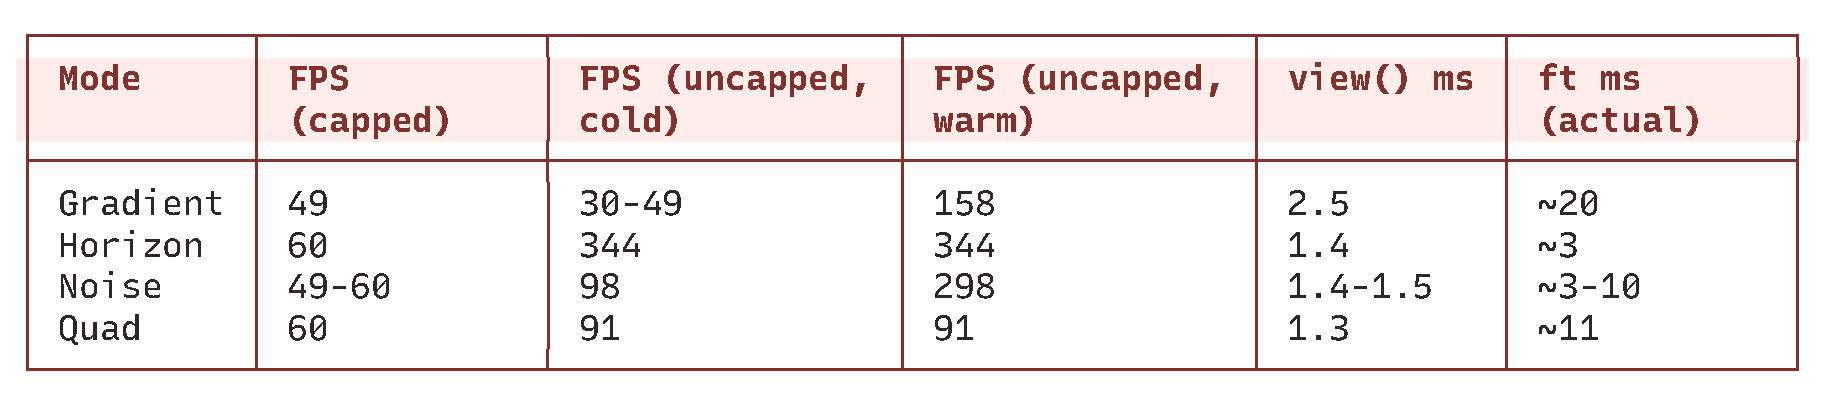
\includegraphics[width=\linewidth]{figures/tables/table-039-g1-1.pdf}
\par\smallskip{\scriptsize\color{BookMuted}Rows 1–4. Actual Bijou table component.}
\end{center}


``Warm'' means after 60+ seconds of sustained rendering, when V8 has JIT-compiled the hot paths and GC has settled.

\section{Where frame time goes}\label{record-156-where-frame-time-goes}

At 191×48 with the gradient (worst case), a frame takes \textasciitilde20ms total:

\begin{center}
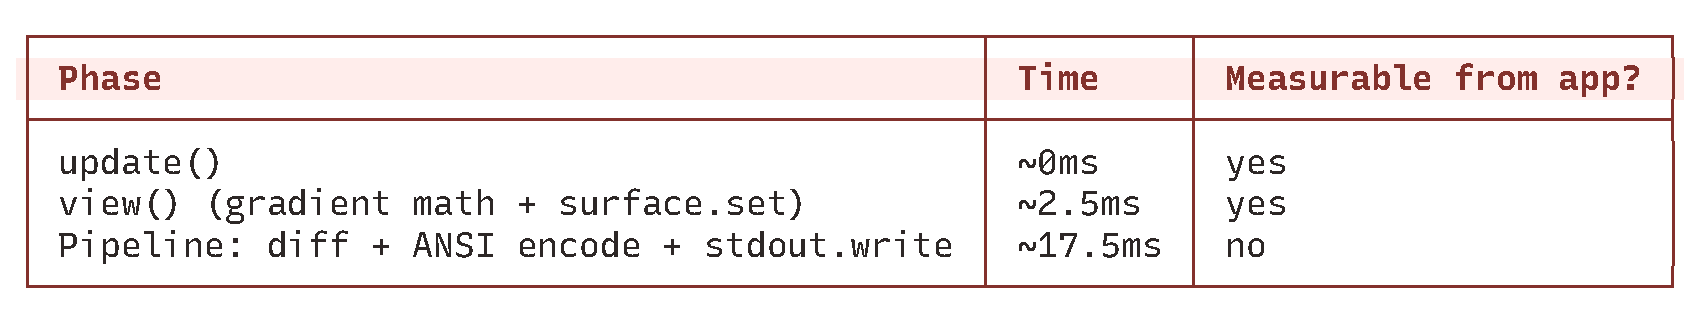
\includegraphics[width=\linewidth]{figures/tables/table-040-g1-1.pdf}
\par\smallskip{\scriptsize\color{BookMuted}Rows 1–3. Actual Bijou table component.}
\end{center}


\textbf{92\% of frame time is spent in bijou's render pipeline, not in the app's view function.} The pipeline is not observable from the app side --- there are no hooks to measure diff, paint, or output phases individually.

\section{The differ is the bottleneck}\label{record-156-the-differ-is-the-bottleneck}

The differ (\texttt{p\allowbreak{}a\allowbreak{}c\allowbreak{}k\allowbreak{}a\allowbreak{}g\allowbreak{}e\allowbreak{}s\allowbreak{}/\allowbreak{}b\allowbreak{}i\allowbreak{}j\allowbreak{}o\allowbreak{}u\allowbreak{}/\allowbreak{}s\allowbreak{}r\allowbreak{}c\allowbreak{}/\allowbreak{}c\allowbreak{}o\allowbreak{}r\allowbreak{}e\allowbreak{}/\allowbreak{}r\allowbreak{}e\allowbreak{}n\allowbreak{}d\allowbreak{}e\allowbreak{}r\allowbreak{}/\allowbreak{}d\allowbreak{}i\allowbreak{}f\allowbreak{}f\allowbreak{}e\allowbreak{}r\allowbreak{}.\allowbreak{}t\allowbreak{}s}) compares every cell in the target surface against the current surface. For cells that changed, it emits ANSI escape sequences.

The differ's performance depends on \textbf{how many unique styles appear in sequence}:

\begin{itemize}
\tightlist
\item
  \textbf{Horizon (344fps uncapped)}: most cells on a row share the same fg/bg, so the differ batches long runs of same-styled characters into single ANSI writes. Very few color change escape sequences per frame.
\item
  \textbf{Noise (298fps uncapped)}: every cell has a unique fg but all share \texttt{b\allowbreak{}g\allowbreak{}:\allowbreak{} \allowbreak{}'\allowbreak{}\#\allowbreak{}0\allowbreak{}0\allowbreak{}0\allowbreak{}0\allowbreak{}0\allowbreak{}0\allowbreak{}'}. The differ still emits per-cell fg changes but saves half the escape sequences (no bg changes).
\item
  \textbf{Gradient (158fps uncapped)}: every cell has a unique fg AND bg. The differ emits \textasciitilde9,168 color change escape sequences per frame --- one per cell. No batching is possible.
\end{itemize}

The differ also compares cells by \textbf{string equality} on \texttt{f\allowbreak{}g} and \texttt{b\allowbreak{}g} hex strings (\texttt{t\allowbreak{}a\allowbreak{}r\allowbreak{}g\allowbreak{}e\allowbreak{}t\allowbreak{}C\allowbreak{}e\allowbreak{}l\allowbreak{}l\allowbreak{}.\allowbreak{}f\allowbreak{}g\allowbreak{} \allowbreak{}=\allowbreak{}=\allowbreak{}=\allowbreak{} \allowbreak{}c\allowbreak{}u\allowbreak{}r\allowbreak{}r\allowbreak{}e\allowbreak{}n\allowbreak{}t\allowbreak{}C\allowbreak{}e\allowbreak{}l\allowbreak{}l\allowbreak{}.\allowbreak{}f\allowbreak{}g}), which is correct but slower than numeric comparison would be.

\section{Allocation pressure and GC}\label{record-156-allocation-pressure-and-gc}

Each \texttt{s\allowbreak{}u\allowbreak{}r\allowbreak{}f\allowbreak{}a\allowbreak{}c\allowbreak{}e\allowbreak{}.\allowbreak{}s\allowbreak{}e\allowbreak{}t\allowbreak{}(\allowbreak{})} call in the gradient mode produces 2 hex color strings (\texttt{r\allowbreak{}g\allowbreak{}b\allowbreak{}H\allowbreak{}e\allowbreak{}x\allowbreak{}(\allowbreak{}r\allowbreak{},\allowbreak{} \allowbreak{}g\allowbreak{},\allowbreak{} \allowbreak{}b\allowbreak{})} for fg and bg). At 9,168 cells per frame, that is \textbf{18,336 string allocations per frame}.

With surface reuse (the cached surface is not reallocated per frame), the Cell objects themselves are mutated in place via \texttt{a\allowbreak{}p\allowbreak{}p\allowbreak{}l\allowbreak{}y\allowbreak{}M\allowbreak{}a\allowbreak{}s\allowbreak{}k\allowbreak{}I\allowbreak{}n\allowbreak{}P\allowbreak{}l\allowbreak{}a\allowbreak{}c\allowbreak{}e}. But the hex color strings are always freshly allocated because they encode the current frame's computed RGB values.

\subsection{GC behavior at different modes}\label{record-156-gc-behavior-at-different-modes}

\begin{center}
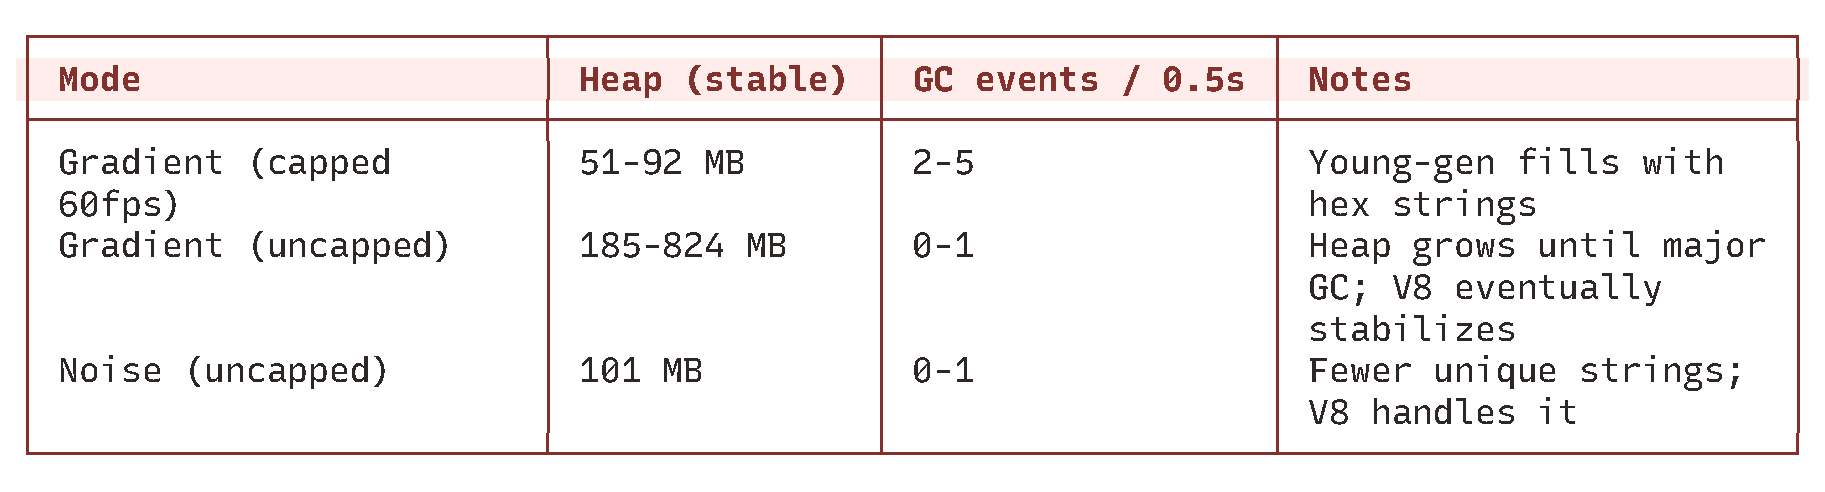
\includegraphics[width=\linewidth]{figures/tables/table-041-g1-1.pdf}
\par\smallskip{\scriptsize\color{BookMuted}Rows 1–3. Actual Bijou table component.}
\end{center}


\subsection{JIT warmup}\label{record-156-jit-warmup}

The gradient mode shows a clear warmup curve:

\begin{itemize}
\tightlist
\item
  \textbf{0-30 seconds}: 30-49fps. V8 is interpreting; GC is aggressive.
\item
  \textbf{30-60 seconds}: 80-120fps. JIT compilation kicks in.
\item
  \textbf{60+ seconds}: 150-160fps. Hot paths fully optimized, GC settled.
\end{itemize}

The noise and horizon modes warm up faster because they produce fewer unique string values per frame.

\section{What RE-008 would fix}\label{record-156-what-re-008-would-fix}

A byte-packed surface representation would eliminate:

\begin{enumerate}
\def\labelenumi{\arabic{enumi}.}
\tightlist
\item
  \textbf{18K string allocations per frame} --- colors stored as 3 bytes (R, G, B), not heap-allocated hex strings.
\item
  \textbf{String comparison in the differ} --- numeric comparison of bytes instead of \texttt{=\allowbreak{}=\allowbreak{}=} on strings.
\item
  \textbf{Hex parsing in the ANSI encoder} --- the \texttt{s\allowbreak{}t\allowbreak{}y\allowbreak{}l\allowbreak{}e\allowbreak{}.\allowbreak{}s\allowbreak{}t\allowbreak{}y\allowbreak{}l\allowbreak{}e\allowbreak{}d\allowbreak{}(\allowbreak{})} call currently parses \texttt{\#\allowbreak{}r\allowbreak{}r\allowbreak{}g\allowbreak{}g\allowbreak{}b\allowbreak{}b} back to numeric RGB to emit \texttt{\textbackslash{}\allowbreak{}x\allowbreak{}1\allowbreak{}b\allowbreak{}[\allowbreak{}3\allowbreak{}8\allowbreak{};\allowbreak{}2\allowbreak{};\allowbreak{}R\allowbreak{};\allowbreak{}G\allowbreak{};\allowbreak{}B\allowbreak{}m}. With byte-packed cells, the encoder reads bytes directly.
\item
  \textbf{The JIT warmup penalty} --- no string-heavy hot paths for V8 to deoptimize and recompile.
\end{enumerate}

\section{What DX-006 would provide}\label{record-156-what-dx-006-would-provide}

A first-class \texttt{d\allowbreak{}e\allowbreak{}b\allowbreak{}u\allowbreak{}g\allowbreak{}O\allowbreak{}v\allowbreak{}e\allowbreak{}r\allowbreak{}l\allowbreak{}a\allowbreak{}y\allowbreak{}(\allowbreak{})} component would let any bijou-tui app see these metrics without rebuilding the stats overlay from scratch. The perf gradient demo proves the concept; DX-006 extracts it into a reusable component.

\section{Pipeline observability gap}\label{record-156-pipeline-observability-gap}

The render pipeline (the illustrated sequence below) is not observable from the app side. \texttt{c\allowbreak{}o\allowbreak{}n\allowbreak{}f\allowbreak{}i\allowbreak{}g\allowbreak{}u\allowbreak{}r\allowbreak{}e\allowbreak{}P\allowbreak{}i\allowbreak{}p\allowbreak{}e\allowbreak{}l\allowbreak{}i\allowbreak{}n\allowbreak{}e} can add middleware but only appends after the default stages --- it cannot wrap them for timing. A future improvement would expose per-stage timing hooks so the debug overlay can show the full breakdown.

% Presentation of original arrow notation. See flow-manifest.json.
\begin{center}
\begin{tikzpicture}[book flow node/.style={draw=BookHeading,line width=.65pt,fill=BookPanel,rounded corners=1.5pt,align=center,inner sep=5pt,minimum height=10mm,font=\fontsize{9}{11}\selectfont,execute at begin node={\hyphenpenalty=10000\exhyphenpenalty=10000}},book flow edge/.style={-{Latex[length=2mm]},draw=BookHeading,line width=.7pt}]
\node[book flow node,text width=96mm] (n0) at (0,0.0) {Layout};
\node[book flow node,text width=96mm] (n1) at (0,-1.55) {Paint};
\node[book flow node,text width=96mm] (n2) at (0,-3.1) {Post\allowbreak{}Process};
\node[book flow node,text width=96mm] (n3) at (0,-4.65) {Diff};
\node[book flow node,text width=96mm] (n4) at (0,-6.2) {Output};
\draw[book flow edge] (n0) -- (n1);
\draw[book flow edge] (n1) -- (n2);
\draw[book flow edge] (n2) -- (n3);
\draw[book flow edge] (n3) -- (n4);
\end{tikzpicture}
\end{center}


\section{Reproducing}\label{record-156-reproducing}

\begin{CodeBlock}
npx tsx examples/perf-gradient/main.ts
\end{CodeBlock}

Keys: \texttt{1\allowbreak{}-\allowbreak{}4} switch modes, \texttt{s\allowbreak{}p\allowbreak{}a\allowbreak{}c\allowbreak{}e} toggles 60fps cap, hold mouse to reverse, \texttt{q} to quit. The stats overlay shows FPS, frame time, view time, heap/RSS/GC, and a braille line chart of view() cost.

%
\chapter{RE-024 Surface Budget Warnings}\label{record-157}

\noindent{\footnotesize\color{BookMuted}\path{docs/design/RE-024-surface-budget-warnings.md}\par}\smallskip

\begin{RecordMeta}
title: RE-024 Surface Budget Warnings
legend: RE
lane: design

\end{RecordMeta}

\section{Framing}\label{record-157-framing}

Many performance regressions are easier to catch during normal development than in a separate benchmark run. Bijou already measures render pipeline timings and owns the target \texttt{S\allowbreak{}u\allowbreak{}r\allowbreak{}f\allowbreak{}a\allowbreak{}c\allowbreak{}e} before diff/output, so the runtime can warn when an app crosses explicit surface or timing budgets.

RE-024 adds opt-in, non-fatal budget diagnostics. The first slice keeps the policy simple: a pure evaluator returns warning objects, and the interactive runtime can route those warnings through the existing \texttt{r\allowbreak{}o\allowbreak{}u\allowbreak{}t\allowbreak{}e\allowbreak{}R\allowbreak{}u\allowbreak{}n\allowbreak{}t\allowbreak{}i\allowbreak{}m\allowbreak{}e\allowbreak{}I\allowbreak{}s\allowbreak{}s\allowbreak{}u\allowbreak{}e} app hook when \texttt{r\allowbreak{}u\allowbreak{}n\allowbreak{}(\allowbreak{}.\allowbreak{}.\allowbreak{}.\allowbreak{},\allowbreak{} \allowbreak{}\{\allowbreak{} \allowbreak{}s\allowbreak{}u\allowbreak{}r\allowbreak{}f\allowbreak{}a\allowbreak{}c\allowbreak{}e\allowbreak{}B\allowbreak{}u\allowbreak{}d\allowbreak{}g\allowbreak{}e\allowbreak{}t\allowbreak{} \allowbreak{}\}\allowbreak{})} is configured.

\section{Sponsored Users}\label{record-157-sponsored-users}

\begin{itemize}
\tightlist
\item
  App authors who want early feedback when a render surface grows beyond an intended size.
\item
  Maintainers reviewing frame timing regressions during normal development.
\item
  Test authors who want deterministic budget warning objects without running a benchmark harness.
\end{itemize}

\section{Hills}\label{record-157-hills}

\begin{enumerate}
\def\labelenumi{\arabic{enumi}.}
\tightlist
\item
  A developer can evaluate a \texttt{S\allowbreak{}u\allowbreak{}r\allowbreak{}f\allowbreak{}a\allowbreak{}c\allowbreak{}e} and render timings against configured budgets and get deterministic warning objects.
\item
  An interactive app can opt into runtime budget warnings without changing its TEA messages unless it chooses to route \texttt{R\allowbreak{}u\allowbreak{}n\allowbreak{}t\allowbreak{}i\allowbreak{}m\allowbreak{}e\allowbreak{}I\allowbreak{}s\allowbreak{}s\allowbreak{}u\allowbreak{}e}s.
\item
  A test can assert that area, styled-cell, frame-duration, and per-stage thresholds produce clear messages.
\end{enumerate}

\section{Playback Questions}\label{record-157-playback-questions}

\begin{itemize}
\tightlist
\item
  Does the pure evaluator stay deterministic and side-effect free?
\item
  Does a target surface over the configured area threshold produce a warning?
\item
  Does a styled-cell count over the configured threshold produce a warning?
\item
  Do frame-duration and stage-duration thresholds use pipeline timings?
\item
  Does \texttt{r\allowbreak{}u\allowbreak{}n\allowbreak{}(\allowbreak{}.\allowbreak{}.\allowbreak{}.\allowbreak{},\allowbreak{} \allowbreak{}\{\allowbreak{} \allowbreak{}s\allowbreak{}u\allowbreak{}r\allowbreak{}f\allowbreak{}a\allowbreak{}c\allowbreak{}e\allowbreak{}B\allowbreak{}u\allowbreak{}d\allowbreak{}g\allowbreak{}e\allowbreak{}t\allowbreak{} \allowbreak{}\}\allowbreak{})} route warnings through \texttt{r\allowbreak{}o\allowbreak{}u\allowbreak{}t\allowbreak{}e\allowbreak{}R\allowbreak{}u\allowbreak{}n\allowbreak{}t\allowbreak{}i\allowbreak{}m\allowbreak{}e\allowbreak{}I\allowbreak{}s\allowbreak{}s\allowbreak{}u\allowbreak{}e} as \texttt{s\allowbreak{}o\allowbreak{}u\allowbreak{}r\allowbreak{}c\allowbreak{}e\allowbreak{}:\allowbreak{} \allowbreak{}'\allowbreak{}r\allowbreak{}u\allowbreak{}n\allowbreak{}t\allowbreak{}i\allowbreak{}m\allowbreak{}e\allowbreak{}'} and \texttt{l\allowbreak{}e\allowbreak{}v\allowbreak{}e\allowbreak{}l\allowbreak{}:\allowbreak{} \allowbreak{}'\allowbreak{}w\allowbreak{}a\allowbreak{}r\allowbreak{}n\allowbreak{}i\allowbreak{}n\allowbreak{}g\allowbreak{}'}?
\item
  Does omitting \texttt{s\allowbreak{}u\allowbreak{}r\allowbreak{}f\allowbreak{}a\allowbreak{}c\allowbreak{}e\allowbreak{}B\allowbreak{}u\allowbreak{}d\allowbreak{}g\allowbreak{}e\allowbreak{}t} keep the runtime silent?
\end{itemize}

\section{Requirements}\label{record-157-requirements}

\begin{itemize}
\tightlist
\item
  Add \texttt{e\allowbreak{}v\allowbreak{}a\allowbreak{}l\allowbreak{}u\allowbreak{}a\allowbreak{}t\allowbreak{}e\allowbreak{}S\allowbreak{}u\allowbreak{}r\allowbreak{}f\allowbreak{}a\allowbreak{}c\allowbreak{}e\allowbreak{}B\allowbreak{}u\allowbreak{}d\allowbreak{}g\allowbreak{}e\allowbreak{}t\allowbreak{}(\allowbreak{})} in \texttt{@\allowbreak{}f\allowbreak{}l\allowbreak{}y\allowbreak{}i\allowbreak{}n\allowbreak{}g\allowbreak{}r\allowbreak{}o\allowbreak{}b\allowbreak{}o\allowbreak{}t\allowbreak{}s\allowbreak{}/\allowbreak{}b\allowbreak{}i\allowbreak{}j\allowbreak{}o\allowbreak{}u\allowbreak{}-\allowbreak{}t\allowbreak{}u\allowbreak{}i}.
\item
  Support maximum width, height, area, styled cells, total frame duration, and per-stage duration thresholds.
\item
  Add \texttt{s\allowbreak{}u\allowbreak{}r\allowbreak{}f\allowbreak{}a\allowbreak{}c\allowbreak{}e\allowbreak{}B\allowbreak{}u\allowbreak{}d\allowbreak{}g\allowbreak{}e\allowbreak{}t} to \texttt{R\allowbreak{}u\allowbreak{}n\allowbreak{}O\allowbreak{}p\allowbreak{}t\allowbreak{}i\allowbreak{}o\allowbreak{}n\allowbreak{}s}.
\item
  Route runtime budget violations through \texttt{r\allowbreak{}o\allowbreak{}u\allowbreak{}t\allowbreak{}e\allowbreak{}R\allowbreak{}u\allowbreak{}n\allowbreak{}t\allowbreak{}i\allowbreak{}m\allowbreak{}e\allowbreak{}I\allowbreak{}s\allowbreak{}s\allowbreak{}u\allowbreak{}e}.
\item
  Keep warnings non-fatal by default.
\end{itemize}

\section{Acceptance Criteria}\label{record-157-acceptance-criteria}

\begin{itemize}
\tightlist
\item
  Focused RED tests fail before implementation and pass after.
\item
  The evaluator returns stable \texttt{S\allowbreak{}u\allowbreak{}r\allowbreak{}f\allowbreak{}a\allowbreak{}c\allowbreak{}e\allowbreak{}B\allowbreak{}u\allowbreak{}d\allowbreak{}g\allowbreak{}e\allowbreak{}t\allowbreak{}W\allowbreak{}a\allowbreak{}r\allowbreak{}n\allowbreak{}i\allowbreak{}n\allowbreak{}g} records.
\item
  Runtime budget warnings use the existing runtime issue route.
\item
  No warning is emitted when no budget is configured.
\item
  Docs and changelog describe the opt-in feature.
\end{itemize}

\section{Implementation Outline}\label{record-157-implementation-outline}

\begin{itemize}
\tightlist
\item
  Implement a pure \texttt{s\allowbreak{}u\allowbreak{}r\allowbreak{}f\allowbreak{}a\allowbreak{}c\allowbreak{}e\allowbreak{}-\allowbreak{}b\allowbreak{}u\allowbreak{}d\allowbreak{}g\allowbreak{}e\allowbreak{}t\allowbreak{}.\allowbreak{}t\allowbreak{}s} helper with threshold and warning types.
\item
  Export the helper and types from the \texttt{b\allowbreak{}i\allowbreak{}j\allowbreak{}o\allowbreak{}u\allowbreak{}-\allowbreak{}t\allowbreak{}u\allowbreak{}i} source barrel.
\item
  Call the helper after pipeline execution, before lifecycle playback, so the warning uses the same target surface and timings that will be committed.
\end{itemize}

\section{Drift Check}\label{record-157-drift-check}

\begin{itemize}
\tightlist
\item
  Scope stayed on non-fatal warnings. The runtime does not fail frames or quit when a threshold is crossed.
\item
  The first slice measures the committed target surface and pipeline timings. Allocation count and output byte volume remain follow-on metrics because they need deeper differ/runtime counters to be accurate.
\item
  Runtime warnings are deduplicated by message to avoid warning/render loops when an app routes budget issues back into its own TEA update path.
\end{itemize}

\section{Playback}\label{record-157-playback}

\begin{itemize}
\tightlist
\item
  \texttt{e\allowbreak{}v\allowbreak{}a\allowbreak{}l\allowbreak{}u\allowbreak{}a\allowbreak{}t\allowbreak{}e\allowbreak{}S\allowbreak{}u\allowbreak{}r\allowbreak{}f\allowbreak{}a\allowbreak{}c\allowbreak{}e\allowbreak{}B\allowbreak{}u\allowbreak{}d\allowbreak{}g\allowbreak{}e\allowbreak{}t\allowbreak{}(\allowbreak{})} returns deterministic warning records for width, height, area, styled-cell count, total frame duration, and per-stage duration.
\item
  \texttt{r\allowbreak{}u\allowbreak{}n\allowbreak{}(\allowbreak{}.\allowbreak{}.\allowbreak{}.\allowbreak{},\allowbreak{} \allowbreak{}\{\allowbreak{} \allowbreak{}s\allowbreak{}u\allowbreak{}r\allowbreak{}f\allowbreak{}a\allowbreak{}c\allowbreak{}e\allowbreak{}B\allowbreak{}u\allowbreak{}d\allowbreak{}g\allowbreak{}e\allowbreak{}t\allowbreak{} \allowbreak{}\}\allowbreak{})} evaluates the target framebuffer after pipeline execution and routes violations through \texttt{r\allowbreak{}o\allowbreak{}u\allowbreak{}t\allowbreak{}e\allowbreak{}R\allowbreak{}u\allowbreak{}n\allowbreak{}t\allowbreak{}i\allowbreak{}m\allowbreak{}e\allowbreak{}I\allowbreak{}s\allowbreak{}s\allowbreak{}u\allowbreak{}e}.
\item
  Runtime warnings use \texttt{l\allowbreak{}e\allowbreak{}v\allowbreak{}e\allowbreak{}l\allowbreak{}:\allowbreak{} \allowbreak{}'\allowbreak{}w\allowbreak{}a\allowbreak{}r\allowbreak{}n\allowbreak{}i\allowbreak{}n\allowbreak{}g\allowbreak{}'} and \texttt{s\allowbreak{}o\allowbreak{}u\allowbreak{}r\allowbreak{}c\allowbreak{}e\allowbreak{}:\allowbreak{} \allowbreak{}'\allowbreak{}r\allowbreak{}u\allowbreak{}n\allowbreak{}t\allowbreak{}i\allowbreak{}m\allowbreak{}e\allowbreak{}'}.
\item
  Omitting \texttt{s\allowbreak{}u\allowbreak{}r\allowbreak{}f\allowbreak{}a\allowbreak{}c\allowbreak{}e\allowbreak{}B\allowbreak{}u\allowbreak{}d\allowbreak{}g\allowbreak{}e\allowbreak{}t} leaves existing runtime behavior unchanged.
\item
  \texttt{@\allowbreak{}f\allowbreak{}l\allowbreak{}y\allowbreak{}i\allowbreak{}n\allowbreak{}g\allowbreak{}r\allowbreak{}o\allowbreak{}b\allowbreak{}o\allowbreak{}t\allowbreak{}s\allowbreak{}/\allowbreak{}b\allowbreak{}i\allowbreak{}j\allowbreak{}o\allowbreak{}u\allowbreak{}-\allowbreak{}t\allowbreak{}u\allowbreak{}i} exports the helper and budget types from the source barrel.
\end{itemize}

\section{Retrospective}\label{record-157-retrospective}

\begin{itemize}
\tightlist
\item
  This is the right first runtime budget boundary: it gives app authors useful early warnings without pretending Bijou can enforce every performance budget from inside the render loop.
\item
  The target surface area is the framebuffer area, not the app view's intrinsic surface size after normalization. Tests pin the viewport when they need exact runtime budget numbers.
\end{itemize}

%
\chapter{RE-030 --- Average High-Resolution Canvas Colors}\label{record-158}

\noindent{\footnotesize\color{BookMuted}\path{docs/design/RE-030-average-high-resolution-canvas-colors.md}\par}\smallskip

Legend: \href{https://github.com/flyingrobots/bijou/blob/1853ad902f6bf219326409e7f743a5a1d6517dbc/docs/legends/RE-runtime-engine.md}{RE --- Runtime Engine}

\section{Sponsor Human}\label{record-158-sponsor-human}

A terminal app builder using \texttt{@\allowbreak{}f\allowbreak{}l\allowbreak{}y\allowbreak{}i\allowbreak{}n\allowbreak{}g\allowbreak{}r\allowbreak{}o\allowbreak{}b\allowbreak{}o\allowbreak{}t\allowbreak{}s\allowbreak{}/\allowbreak{}b\allowbreak{}i\allowbreak{}j\allowbreak{}o\allowbreak{}u\allowbreak{}-\allowbreak{}t\allowbreak{}u\allowbreak{}i} canvas shaders for small procedural images, title screens, charts, and textured scene previews.

\section{Sponsor Agent}\label{record-158-sponsor-agent}

An implementation agent that must render high-density terminal art without repairing colors after the canvas has already collapsed subpixels into cells.

\section{Hills}\label{record-158-hills}

\begin{enumerate}
\def\labelenumi{\arabic{enumi}.}
\tightlist
\item
  A builder can return per-subpixel RGB values from a \texttt{c\allowbreak{}a\allowbreak{}n\allowbreak{}v\allowbreak{}a\allowbreak{}s\allowbreak{}(\allowbreak{})} shader and trust Bijou to collapse those colors the way image resampling normally does.
\item
  A builder can use \texttt{b\allowbreak{}r\allowbreak{}a\allowbreak{}i\allowbreak{}l\allowbreak{}l\allowbreak{}e} or \texttt{q\allowbreak{}u\allowbreak{}a\allowbreak{}d} resolution without losing color when the first lit subpixel is not representative of the whole terminal cell.
\item
  An agent can debug canvas color behavior from \texttt{c\allowbreak{}a\allowbreak{}n\allowbreak{}v\allowbreak{}a\allowbreak{}s\allowbreak{}.\allowbreak{}t\allowbreak{}s} itself rather than recommending app-local post-render \texttt{s\allowbreak{}e\allowbreak{}t\allowbreak{}R\allowbreak{}G\allowbreak{}B\allowbreak{}(\allowbreak{})} correction loops.
\end{enumerate}

\section{Playback Questions}\label{record-158-playback-questions}

\begin{enumerate}
\def\labelenumi{\arabic{enumi}.}
\tightlist
\item
  In \texttt{b\allowbreak{}r\allowbreak{}a\allowbreak{}i\allowbreak{}l\allowbreak{}l\allowbreak{}e} mode, when eight subpixels return different foreground RGB values, does the resulting Braille cell use their arithmetic mean?
\item
  In \texttt{b\allowbreak{}r\allowbreak{}a\allowbreak{}i\allowbreak{}l\allowbreak{}l\allowbreak{}e} mode, when all eight subpixels are visually off but still return background RGB values, does the collapsed cell preserve their average background style?
\item
  In \texttt{q\allowbreak{}u\allowbreak{}a\allowbreak{}d} mode, when four subpixels return different RGB values, does the resulting quadrant character use the arithmetic mean instead of the first lit subpixel's style?
\item
  Does the character coverage behavior stay unchanged while only style aggregation changes?
\end{enumerate}

\section{Requirements}\label{record-158-requirements}

\begin{itemize}
\tightlist
\item
  \texttt{c\allowbreak{}a\allowbreak{}n\allowbreak{}v\allowbreak{}a\allowbreak{}s\allowbreak{}(\allowbreak{}.\allowbreak{}.\allowbreak{}.\allowbreak{},\allowbreak{} \allowbreak{}\{\allowbreak{} \allowbreak{}r\allowbreak{}e\allowbreak{}s\allowbreak{}o\allowbreak{}l\allowbreak{}u\allowbreak{}t\allowbreak{}i\allowbreak{}o\allowbreak{}n\allowbreak{}:\allowbreak{} \allowbreak{}'\allowbreak{}b\allowbreak{}r\allowbreak{}a\allowbreak{}i\allowbreak{}l\allowbreak{}l\allowbreak{}e\allowbreak{}'\allowbreak{} \allowbreak{}\}\allowbreak{})} must sample all 2x4 subpixels for the output cell and average every available foreground RGB contribution.
\item
  \texttt{c\allowbreak{}a\allowbreak{}n\allowbreak{}v\allowbreak{}a\allowbreak{}s\allowbreak{}(\allowbreak{}.\allowbreak{}.\allowbreak{}.\allowbreak{},\allowbreak{} \allowbreak{}\{\allowbreak{} \allowbreak{}r\allowbreak{}e\allowbreak{}s\allowbreak{}o\allowbreak{}l\allowbreak{}u\allowbreak{}t\allowbreak{}i\allowbreak{}o\allowbreak{}n\allowbreak{}:\allowbreak{} \allowbreak{}'\allowbreak{}b\allowbreak{}r\allowbreak{}a\allowbreak{}i\allowbreak{}l\allowbreak{}l\allowbreak{}e\allowbreak{}'\allowbreak{} \allowbreak{}\}\allowbreak{})} must also average every available background RGB contribution, including cells whose shader character is a space.
\item
  \texttt{c\allowbreak{}a\allowbreak{}n\allowbreak{}v\allowbreak{}a\allowbreak{}s\allowbreak{}(\allowbreak{}.\allowbreak{}.\allowbreak{}.\allowbreak{},\allowbreak{} \allowbreak{}\{\allowbreak{} \allowbreak{}r\allowbreak{}e\allowbreak{}s\allowbreak{}o\allowbreak{}l\allowbreak{}u\allowbreak{}t\allowbreak{}i\allowbreak{}o\allowbreak{}n\allowbreak{}:\allowbreak{} \allowbreak{}'\allowbreak{}q\allowbreak{}u\allowbreak{}a\allowbreak{}d\allowbreak{}'\allowbreak{} \allowbreak{}\}\allowbreak{})} must use the same color aggregation rule across its 2x2 subpixels.
\item
  Shader results that return \texttt{f\allowbreak{}g\allowbreak{}R\allowbreak{}G\allowbreak{}B} or \texttt{b\allowbreak{}g\allowbreak{}R\allowbreak{}G\allowbreak{}B} must avoid unnecessary hex parsing.
\item
  Shader results that return parseable hex or resolved color references must still participate in the same averaging path.
\item
  Coverage remains boolean: non-space subpixels set Braille dots or quadrant bits, and space subpixels leave those dots or bits off.
\item
  Modifiers remain compatibility-oriented and come from the first lit styled subpixel.
\end{itemize}

\section{Acceptance Criteria}\label{record-158-acceptance-criteria}

\begin{itemize}
\tightlist
\item
  Red tests prove Braille foreground averaging, Braille background averaging for an empty Braille cell, and Quad foreground averaging.
\item
  The implementation changes \texttt{p\allowbreak{}a\allowbreak{}c\allowbreak{}k\allowbreak{}a\allowbreak{}g\allowbreak{}e\allowbreak{}s\allowbreak{}/\allowbreak{}b\allowbreak{}i\allowbreak{}j\allowbreak{}o\allowbreak{}u\allowbreak{}-\allowbreak{}t\allowbreak{}u\allowbreak{}i\allowbreak{}/\allowbreak{}s\allowbreak{}r\allowbreak{}c\allowbreak{}/\allowbreak{}c\allowbreak{}a\allowbreak{}n\allowbreak{}v\allowbreak{}a\allowbreak{}s\allowbreak{}.\allowbreak{}t\allowbreak{}s} instead of requiring app-local post-processing.
\item
  \texttt{n\allowbreak{}p\allowbreak{}m\allowbreak{} \allowbreak{}r\allowbreak{}u\allowbreak{}n\allowbreak{} \allowbreak{}t\allowbreak{}e\allowbreak{}s\allowbreak{}t\allowbreak{} \allowbreak{}-\allowbreak{}-\allowbreak{} \allowbreak{}p\allowbreak{}a\allowbreak{}c\allowbreak{}k\allowbreak{}a\allowbreak{}g\allowbreak{}e\allowbreak{}s\allowbreak{}/\allowbreak{}b\allowbreak{}i\allowbreak{}j\allowbreak{}o\allowbreak{}u\allowbreak{}-\allowbreak{}t\allowbreak{}u\allowbreak{}i\allowbreak{}/\allowbreak{}s\allowbreak{}r\allowbreak{}c\allowbreak{}/\allowbreak{}c\allowbreak{}a\allowbreak{}n\allowbreak{}v\allowbreak{}a\allowbreak{}s\allowbreak{}.\allowbreak{}t\allowbreak{}e\allowbreak{}s\allowbreak{}t\allowbreak{}.\allowbreak{}t\allowbreak{}s} passes.
\item
  \texttt{n\allowbreak{}p\allowbreak{}m\allowbreak{} \allowbreak{}r\allowbreak{}u\allowbreak{}n\allowbreak{} \allowbreak{}l\allowbreak{}i\allowbreak{}n\allowbreak{}t\allowbreak{} \allowbreak{}-\allowbreak{}-\allowbreak{}w\allowbreak{}o\allowbreak{}r\allowbreak{}k\allowbreak{}s\allowbreak{}p\allowbreak{}a\allowbreak{}c\allowbreak{}e\allowbreak{} \allowbreak{}@\allowbreak{}f\allowbreak{}l\allowbreak{}y\allowbreak{}i\allowbreak{}n\allowbreak{}g\allowbreak{}r\allowbreak{}o\allowbreak{}b\allowbreak{}o\allowbreak{}t\allowbreak{}s\allowbreak{}/\allowbreak{}b\allowbreak{}i\allowbreak{}j\allowbreak{}o\allowbreak{}u\allowbreak{}-\allowbreak{}t\allowbreak{}u\allowbreak{}i} passes.
\item
  \texttt{g\allowbreak{}i\allowbreak{}t\allowbreak{} \allowbreak{}d\allowbreak{}i\allowbreak{}f\allowbreak{}f\allowbreak{} \allowbreak{}-\allowbreak{}-\allowbreak{}c\allowbreak{}h\allowbreak{}e\allowbreak{}c\allowbreak{}k} passes.
\end{itemize}

\section{Accessibility / Assistive Reading Posture}\label{record-158-accessibility-assistive-reading-posture}

This change preserves character semantics and only adjusts styling. Existing plain text and assistive interpretations of the character grid should remain unchanged.

\section{Localization / Directionality Posture}\label{record-158-localization-directionality-posture}

The feature is independent of prose localization and bidirectional text. It does not alter grapheme ordering or directional layout.

\section{Agent Inspectability / Explainability Posture}\label{record-158-agent-inspectability-explainability-posture}

The color decision must live in named helper functions in \texttt{c\allowbreak{}a\allowbreak{}n\allowbreak{}v\allowbreak{}a\allowbreak{}s\allowbreak{}.\allowbreak{}t\allowbreak{}s}, with tests that make the sampling rule explicit. Agents should be able to explain that the high-resolution renderer computes coverage and style separately: coverage chooses the Braille or quadrant glyph, while style is averaged from sampled subpixel styles.

\section{Linked Invariants}\label{record-158-linked-invariants}

\begin{itemize}
\tightlist
\item
  \href{https://github.com/flyingrobots/bijou/blob/cbd70612140e7a450d764b3c7be1c6af878b99bc/docs/invariants/tests-are-the-spec.md}{Tests Are the Spec}
\item
  \href{https://github.com/flyingrobots/bijou/blob/cbd70612140e7a450d764b3c7be1c6af878b99bc/docs/invariants/runtime-truth-wins.md}{Runtime Truth Wins}
\end{itemize}

\section{Implementation Outline}\label{record-158-implementation-outline}

\begin{enumerate}
\def\labelenumi{\arabic{enumi}.}
\tightlist
\item
  Add failing tests for Braille foreground averaging, empty-cell background averaging, and Quad foreground averaging.
\item
  Introduce a small color accumulator in \texttt{c\allowbreak{}a\allowbreak{}n\allowbreak{}v\allowbreak{}a\allowbreak{}s\allowbreak{}.\allowbreak{}t\allowbreak{}s}.
\item
  Resolve each sampled cell's foreground and background color from \texttt{f\allowbreak{}g\allowbreak{}R\allowbreak{}G\allowbreak{}B}, \texttt{b\allowbreak{}g\allowbreak{}R\allowbreak{}G\allowbreak{}B}, resolved color refs, or parseable hex strings.
\item
  Average available foreground and background samples independently using rounded arithmetic means.
\item
  Apply the averaged style to the collapsed Braille or Quad cell while preserving existing coverage behavior.
\end{enumerate}

\section{Tests To Write First}\label{record-158-tests-to-write-first}

\begin{itemize}
\tightlist
\item
  \texttt{a\allowbreak{}v\allowbreak{}e\allowbreak{}r\allowbreak{}a\allowbreak{}g\allowbreak{}e\allowbreak{}s\allowbreak{} \allowbreak{}b\allowbreak{}r\allowbreak{}a\allowbreak{}i\allowbreak{}l\allowbreak{}l\allowbreak{}e\allowbreak{} \allowbreak{}s\allowbreak{}u\allowbreak{}b\allowbreak{}-\allowbreak{}p\allowbreak{}i\allowbreak{}x\allowbreak{}e\allowbreak{}l\allowbreak{} \allowbreak{}f\allowbreak{}o\allowbreak{}r\allowbreak{}e\allowbreak{}g\allowbreak{}r\allowbreak{}o\allowbreak{}u\allowbreak{}n\allowbreak{}d\allowbreak{} \allowbreak{}c\allowbreak{}o\allowbreak{}l\allowbreak{}o\allowbreak{}r\allowbreak{}s}
\item
  \texttt{p\allowbreak{}r\allowbreak{}e\allowbreak{}s\allowbreak{}e\allowbreak{}r\allowbreak{}v\allowbreak{}e\allowbreak{}s\allowbreak{} \allowbreak{}a\allowbreak{}v\allowbreak{}e\allowbreak{}r\allowbreak{}a\allowbreak{}g\allowbreak{}e\allowbreak{}d\allowbreak{} \allowbreak{}b\allowbreak{}r\allowbreak{}a\allowbreak{}i\allowbreak{}l\allowbreak{}l\allowbreak{}e\allowbreak{} \allowbreak{}b\allowbreak{}a\allowbreak{}c\allowbreak{}k\allowbreak{}g\allowbreak{}r\allowbreak{}o\allowbreak{}u\allowbreak{}n\allowbreak{}d\allowbreak{} \allowbreak{}c\allowbreak{}o\allowbreak{}l\allowbreak{}o\allowbreak{}r\allowbreak{}s\allowbreak{} \allowbreak{}f\allowbreak{}o\allowbreak{}r\allowbreak{} \allowbreak{}e\allowbreak{}m\allowbreak{}p\allowbreak{}t\allowbreak{}y\allowbreak{} \allowbreak{}c\allowbreak{}e\allowbreak{}l\allowbreak{}l\allowbreak{}s}
\item
  \texttt{a\allowbreak{}v\allowbreak{}e\allowbreak{}r\allowbreak{}a\allowbreak{}g\allowbreak{}e\allowbreak{}s\allowbreak{} \allowbreak{}q\allowbreak{}u\allowbreak{}a\allowbreak{}d\allowbreak{} \allowbreak{}s\allowbreak{}u\allowbreak{}b\allowbreak{}-\allowbreak{}p\allowbreak{}i\allowbreak{}x\allowbreak{}e\allowbreak{}l\allowbreak{} \allowbreak{}f\allowbreak{}o\allowbreak{}r\allowbreak{}e\allowbreak{}g\allowbreak{}r\allowbreak{}o\allowbreak{}u\allowbreak{}n\allowbreak{}d\allowbreak{} \allowbreak{}c\allowbreak{}o\allowbreak{}l\allowbreak{}o\allowbreak{}r\allowbreak{}s}
\end{itemize}

\section{Drift Check}\label{record-158-drift-check}

\begin{itemize}
\tightlist
\item
  RED observed: \texttt{n\allowbreak{}p\allowbreak{}m\allowbreak{} \allowbreak{}r\allowbreak{}u\allowbreak{}n\allowbreak{} \allowbreak{}t\allowbreak{}e\allowbreak{}s\allowbreak{}t\allowbreak{} \allowbreak{}-\allowbreak{}-\allowbreak{} \allowbreak{}p\allowbreak{}a\allowbreak{}c\allowbreak{}k\allowbreak{}a\allowbreak{}g\allowbreak{}e\allowbreak{}s\allowbreak{}/\allowbreak{}b\allowbreak{}i\allowbreak{}j\allowbreak{}o\allowbreak{}u\allowbreak{}-\allowbreak{}t\allowbreak{}u\allowbreak{}i\allowbreak{}/\allowbreak{}s\allowbreak{}r\allowbreak{}c\allowbreak{}/\allowbreak{}c\allowbreak{}a\allowbreak{}n\allowbreak{}v\allowbreak{}a\allowbreak{}s\allowbreak{}.\allowbreak{}t\allowbreak{}e\allowbreak{}s\allowbreak{}t\allowbreak{}.\allowbreak{}t\allowbreak{}s} failed with three expected assertions: Braille foreground used \texttt{[\allowbreak{}0\allowbreak{},\allowbreak{} \allowbreak{}0\allowbreak{},\allowbreak{} \allowbreak{}0\allowbreak{}]}, empty Braille background was \texttt{u\allowbreak{}n\allowbreak{}d\allowbreak{}e\allowbreak{}f\allowbreak{}i\allowbreak{}n\allowbreak{}e\allowbreak{}d}, and Quad foreground used \texttt{[\allowbreak{}0\allowbreak{},\allowbreak{} \allowbreak{}0\allowbreak{},\allowbreak{} \allowbreak{}0\allowbreak{}]}.
\item
  GREEN observed: \texttt{n\allowbreak{}p\allowbreak{}m\allowbreak{} \allowbreak{}r\allowbreak{}u\allowbreak{}n\allowbreak{} \allowbreak{}t\allowbreak{}e\allowbreak{}s\allowbreak{}t\allowbreak{} \allowbreak{}-\allowbreak{}-\allowbreak{} \allowbreak{}p\allowbreak{}a\allowbreak{}c\allowbreak{}k\allowbreak{}a\allowbreak{}g\allowbreak{}e\allowbreak{}s\allowbreak{}/\allowbreak{}b\allowbreak{}i\allowbreak{}j\allowbreak{}o\allowbreak{}u\allowbreak{}-\allowbreak{}t\allowbreak{}u\allowbreak{}i\allowbreak{}/\allowbreak{}s\allowbreak{}r\allowbreak{}c\allowbreak{}/\allowbreak{}c\allowbreak{}a\allowbreak{}n\allowbreak{}v\allowbreak{}a\allowbreak{}s\allowbreak{}.\allowbreak{}t\allowbreak{}e\allowbreak{}s\allowbreak{}t\allowbreak{}.\allowbreak{}t\allowbreak{}s} passed with 9 tests.
\item
  Package lint observed: \texttt{n\allowbreak{}p\allowbreak{}m\allowbreak{} \allowbreak{}r\allowbreak{}u\allowbreak{}n\allowbreak{} \allowbreak{}l\allowbreak{}i\allowbreak{}n\allowbreak{}t\allowbreak{} \allowbreak{}-\allowbreak{}-\allowbreak{}w\allowbreak{}o\allowbreak{}r\allowbreak{}k\allowbreak{}s\allowbreak{}p\allowbreak{}a\allowbreak{}c\allowbreak{}e\allowbreak{} \allowbreak{}@\allowbreak{}f\allowbreak{}l\allowbreak{}y\allowbreak{}i\allowbreak{}n\allowbreak{}g\allowbreak{}r\allowbreak{}o\allowbreak{}b\allowbreak{}o\allowbreak{}t\allowbreak{}s\allowbreak{}/\allowbreak{}b\allowbreak{}i\allowbreak{}j\allowbreak{}o\allowbreak{}u\allowbreak{}-\allowbreak{}t\allowbreak{}u\allowbreak{}i} passed.
\item
  Root lint: \texttt{n\allowbreak{}p\allowbreak{}m\allowbreak{} \allowbreak{}r\allowbreak{}u\allowbreak{}n\allowbreak{} \allowbreak{}l\allowbreak{}i\allowbreak{}n\allowbreak{}t} reached the workspace sweep but failed on pre-existing uncommitted \texttt{p\allowbreak{}a\allowbreak{}c\allowbreak{}k\allowbreak{}a\allowbreak{}g\allowbreak{}e\allowbreak{}s\allowbreak{}/\allowbreak{}h\allowbreak{}e\allowbreak{}a\allowbreak{}t\allowbreak{}m\allowbreak{}a\allowbreak{}p} work because \texttt{@\allowbreak{}f\allowbreak{}l\allowbreak{}y\allowbreak{}i\allowbreak{}n\allowbreak{}g\allowbreak{}r\allowbreak{}o\allowbreak{}b\allowbreak{}o\allowbreak{}t\allowbreak{}s\allowbreak{}/\allowbreak{}b\allowbreak{}i\allowbreak{}j\allowbreak{}o\allowbreak{}u\allowbreak{}-\allowbreak{}h\allowbreak{}e\allowbreak{}a\allowbreak{}t\allowbreak{}m\allowbreak{}a\allowbreak{}p} had no \texttt{l\allowbreak{}i\allowbreak{}n\allowbreak{}t} script. After the local heatmap workspace drift was repaired, \texttt{n\allowbreak{}p\allowbreak{}m\allowbreak{} \allowbreak{}r\allowbreak{}u\allowbreak{}n\allowbreak{} \allowbreak{}l\allowbreak{}i\allowbreak{}n\allowbreak{}t} passed.
\item
  Pre-commit lockfile gate: \texttt{n\allowbreak{}p\allowbreak{}m\allowbreak{} \allowbreak{}l\allowbreak{}s\allowbreak{} \allowbreak{}-\allowbreak{}-\allowbreak{}a\allowbreak{}l\allowbreak{}l} still fails in the local install tree with extraneous and missing dependency reports unrelated to this canvas change, so the scoped commit used the recorded tests and lint results rather than treating local install drift as RE-030 scope.
\item
  Whitespace drift: \texttt{g\allowbreak{}i\allowbreak{}t\allowbreak{} \allowbreak{}d\allowbreak{}i\allowbreak{}f\allowbreak{}f\allowbreak{} \allowbreak{}-\allowbreak{}-\allowbreak{}c\allowbreak{}h\allowbreak{}e\allowbreak{}c\allowbreak{}k} passed.
\end{itemize}

\section{Playback}\label{record-158-playback}

\begin{enumerate}
\def\labelenumi{\arabic{enumi}.}
\tightlist
\item
  Braille foreground averaging is covered by \texttt{a\allowbreak{}v\allowbreak{}e\allowbreak{}r\allowbreak{}a\allowbreak{}g\allowbreak{}e\allowbreak{}s\allowbreak{} \allowbreak{}b\allowbreak{}r\allowbreak{}a\allowbreak{}i\allowbreak{}l\allowbreak{}l\allowbreak{}e\allowbreak{} \allowbreak{}s\allowbreak{}u\allowbreak{}b\allowbreak{}-\allowbreak{}p\allowbreak{}i\allowbreak{}x\allowbreak{}e\allowbreak{}l\allowbreak{} \allowbreak{}f\allowbreak{}o\allowbreak{}r\allowbreak{}e\allowbreak{}g\allowbreak{}r\allowbreak{}o\allowbreak{}u\allowbreak{}n\allowbreak{}d\allowbreak{} \allowbreak{}c\allowbreak{}o\allowbreak{}l\allowbreak{}o\allowbreak{}r\allowbreak{}s}; the collapsed full Braille cell now carries \texttt{[\allowbreak{}2\allowbreak{}8\allowbreak{},\allowbreak{} \allowbreak{}5\allowbreak{}6\allowbreak{},\allowbreak{} \allowbreak{}8\allowbreak{}4\allowbreak{}]} from eight RGB samples.
\item
  Empty Braille background preservation is covered by \texttt{p\allowbreak{}r\allowbreak{}e\allowbreak{}s\allowbreak{}e\allowbreak{}r\allowbreak{}v\allowbreak{}e\allowbreak{}s\allowbreak{} \allowbreak{}a\allowbreak{}v\allowbreak{}e\allowbreak{}r\allowbreak{}a\allowbreak{}g\allowbreak{}e\allowbreak{}d\allowbreak{} \allowbreak{}b\allowbreak{}r\allowbreak{}a\allowbreak{}i\allowbreak{}l\allowbreak{}l\allowbreak{}e\allowbreak{} \allowbreak{}b\allowbreak{}a\allowbreak{}c\allowbreak{}k\allowbreak{}g\allowbreak{}r\allowbreak{}o\allowbreak{}u\allowbreak{}n\allowbreak{}d\allowbreak{} \allowbreak{}c\allowbreak{}o\allowbreak{}l\allowbreak{}o\allowbreak{}r\allowbreak{}s\allowbreak{} \allowbreak{}f\allowbreak{}o\allowbreak{}r\allowbreak{} \allowbreak{}e\allowbreak{}m\allowbreak{}p\allowbreak{}t\allowbreak{}y\allowbreak{} \allowbreak{}c\allowbreak{}e\allowbreak{}l\allowbreak{}l\allowbreak{}s}; the blank Braille cell now carries \texttt{[\allowbreak{}2\allowbreak{}8\allowbreak{},\allowbreak{} \allowbreak{}3\allowbreak{}8\allowbreak{},\allowbreak{} \allowbreak{}4\allowbreak{}8\allowbreak{}]} even when no dot is lit.
\item
  Quad foreground averaging is covered by \texttt{a\allowbreak{}v\allowbreak{}e\allowbreak{}r\allowbreak{}a\allowbreak{}g\allowbreak{}e\allowbreak{}s\allowbreak{} \allowbreak{}q\allowbreak{}u\allowbreak{}a\allowbreak{}d\allowbreak{} \allowbreak{}s\allowbreak{}u\allowbreak{}b\allowbreak{}-\allowbreak{}p\allowbreak{}i\allowbreak{}x\allowbreak{}e\allowbreak{}l\allowbreak{} \allowbreak{}f\allowbreak{}o\allowbreak{}r\allowbreak{}e\allowbreak{}g\allowbreak{}r\allowbreak{}o\allowbreak{}u\allowbreak{}n\allowbreak{}d\allowbreak{} \allowbreak{}c\allowbreak{}o\allowbreak{}l\allowbreak{}o\allowbreak{}r\allowbreak{}s}; the \texttt{▚} glyph now carries \texttt{[\allowbreak{}1\allowbreak{}5\allowbreak{},\allowbreak{} \allowbreak{}3\allowbreak{}0\allowbreak{},\allowbreak{} \allowbreak{}4\allowbreak{}5\allowbreak{}]} from all four samples.
\item
  Existing coverage tests for top-left Braille and diagonal Quad glyphs still pass, so glyph selection stayed stable while style aggregation changed.
\end{enumerate}

\section{Retrospective}\label{record-158-retrospective}

The root issue was local to high-resolution canvas style aggregation. The renderer already sampled the right subpixels for coverage but treated style as a first-lit-subpixel property. Splitting coverage from style lets shader authors return material colors per sample and lets Bijou perform the terminal-cell resampling step itself. No app should need to walk the rendered surface after \texttt{c\allowbreak{}a\allowbreak{}n\allowbreak{}v\allowbreak{}a\allowbreak{}s\allowbreak{}(\allowbreak{})} just to recover colors.

%
\chapter{RE-031 --- Raytrace Shader Kernel}\label{record-159}

\noindent{\footnotesize\color{BookMuted}\path{docs/design/RE-031-raytrace-shader-kernel.md}\par}\smallskip

Legend: \href{https://github.com/flyingrobots/bijou/blob/1853ad902f6bf219326409e7f743a5a1d6517dbc/docs/legends/RE-runtime-engine.md}{RE --- Runtime Engine}

\section{Sponsor Human}\label{record-159-sponsor-human}

A Bijou app builder creating title screens, procedural previews, or small shader-driven scenes in terminal cells.

\section{Sponsor Agent}\label{record-159-sponsor-agent}

An implementation agent that needs to author terminal ray scenes without copying vector math, camera rays, sphere intersections, and reflection helpers into each app.

\section{Hills}\label{record-159-hills}

\begin{enumerate}
\def\labelenumi{\arabic{enumi}.}
\tightlist
\item
  A builder can import a tiny raytrace kernel from \texttt{@\allowbreak{}f\allowbreak{}l\allowbreak{}y\allowbreak{}i\allowbreak{}n\allowbreak{}g\allowbreak{}r\allowbreak{}o\allowbreak{}b\allowbreak{}o\allowbreak{}t\allowbreak{}s\allowbreak{}/\allowbreak{}b\allowbreak{}i\allowbreak{}j\allowbreak{}o\allowbreak{}u\allowbreak{}-\allowbreak{}t\allowbreak{}u\allowbreak{}i} and use it inside \texttt{c\allowbreak{}a\allowbreak{}n\allowbreak{}v\allowbreak{}a\allowbreak{}s\allowbreak{}(\allowbreak{})} shaders without pulling in an external 3D engine.
\item
  A builder can keep app-specific material and lighting decisions local while sharing the boring, error-prone geometry math.
\item
  An agent can factor a title-screen ray tracer into reusable Bijou helpers without turning Bijou into a full scene graph or renderer.
\end{enumerate}

\section{Playback Questions}\label{record-159-playback-questions}

\begin{enumerate}
\def\labelenumi{\arabic{enumi}.}
\tightlist
\item
  Can a caller create a look-at camera ray whose center sample points from the camera origin to the target?
\item
  Can the kernel report the first positive sphere hit with correct distance, hit point, and surface normal?
\item
  Can the kernel compare supported shapes and return the nearest hit?
\item
  Can reflection math be reused by app-specific lighting code without the app reimplementing vector operations?
\end{enumerate}

\section{Requirements}\label{record-159-requirements}

\begin{itemize}
\tightlist
\item
  Export \texttt{R\allowbreak{}a\allowbreak{}y\allowbreak{}t\allowbreak{}r\allowbreak{}a\allowbreak{}c\allowbreak{}e\allowbreak{}V\allowbreak{}e\allowbreak{}c\allowbreak{}t\allowbreak{}o\allowbreak{}r\allowbreak{}3}, \texttt{R\allowbreak{}a\allowbreak{}y\allowbreak{}t\allowbreak{}r\allowbreak{}a\allowbreak{}c\allowbreak{}e\allowbreak{}R\allowbreak{}a\allowbreak{}y}, \texttt{R\allowbreak{}a\allowbreak{}y\allowbreak{}t\allowbreak{}r\allowbreak{}a\allowbreak{}c\allowbreak{}e\allowbreak{}S\allowbreak{}p\allowbreak{}h\allowbreak{}e\allowbreak{}r\allowbreak{}e}, \texttt{R\allowbreak{}a\allowbreak{}y\allowbreak{}t\allowbreak{}r\allowbreak{}a\allowbreak{}c\allowbreak{}e\allowbreak{}P\allowbreak{}l\allowbreak{}a\allowbreak{}n\allowbreak{}e}, \texttt{R\allowbreak{}a\allowbreak{}y\allowbreak{}t\allowbreak{}r\allowbreak{}a\allowbreak{}c\allowbreak{}e\allowbreak{}S\allowbreak{}h\allowbreak{}a\allowbreak{}p\allowbreak{}e}, and \texttt{R\allowbreak{}a\allowbreak{}y\allowbreak{}t\allowbreak{}r\allowbreak{}a\allowbreak{}c\allowbreak{}e\allowbreak{}H\allowbreak{}i\allowbreak{}t} types from \texttt{@\allowbreak{}f\allowbreak{}l\allowbreak{}y\allowbreak{}i\allowbreak{}n\allowbreak{}g\allowbreak{}r\allowbreak{}o\allowbreak{}b\allowbreak{}o\allowbreak{}t\allowbreak{}s\allowbreak{}/\allowbreak{}b\allowbreak{}i\allowbreak{}j\allowbreak{}o\allowbreak{}u\allowbreak{}-\allowbreak{}t\allowbreak{}u\allowbreak{}i}.
\item
  Export pure vector helpers for add, subtract, scale, dot, cross, normalize, reflect, and mix-in camera composition.
\item
  Provide a \texttt{r\allowbreak{}a\allowbreak{}y\allowbreak{}t\allowbreak{}r\allowbreak{}a\allowbreak{}c\allowbreak{}e\allowbreak{}L\allowbreak{}o\allowbreak{}o\allowbreak{}k\allowbreak{}A\allowbreak{}t\allowbreak{}R\allowbreak{}a\allowbreak{}y\allowbreak{}(\allowbreak{})} helper that builds a normalized ray from an origin, target, screen coordinate, and focal length.
\item
  Provide a \texttt{r\allowbreak{}a\allowbreak{}y\allowbreak{}t\allowbreak{}r\allowbreak{}a\allowbreak{}c\allowbreak{}e\allowbreak{}O\allowbreak{}r\allowbreak{}b\allowbreak{}i\allowbreak{}t\allowbreak{}C\allowbreak{}a\allowbreak{}m\allowbreak{}e\allowbreak{}r\allowbreak{}a\allowbreak{}R\allowbreak{}a\allowbreak{}y\allowbreak{}(\allowbreak{})} helper for the common orbiting title screen camera pattern.
\item
  Provide \texttt{r\allowbreak{}a\allowbreak{}y\allowbreak{}t\allowbreak{}r\allowbreak{}a\allowbreak{}c\allowbreak{}e\allowbreak{}S\allowbreak{}p\allowbreak{}h\allowbreak{}e\allowbreak{}r\allowbreak{}e\allowbreak{}H\allowbreak{}i\allowbreak{}t\allowbreak{}(\allowbreak{})}, \texttt{r\allowbreak{}a\allowbreak{}y\allowbreak{}t\allowbreak{}r\allowbreak{}a\allowbreak{}c\allowbreak{}e\allowbreak{}P\allowbreak{}l\allowbreak{}a\allowbreak{}n\allowbreak{}e\allowbreak{}H\allowbreak{}i\allowbreak{}t\allowbreak{}(\allowbreak{})}, and \texttt{r\allowbreak{}a\allowbreak{}y\allowbreak{}t\allowbreak{}r\allowbreak{}a\allowbreak{}c\allowbreak{}e\allowbreak{}N\allowbreak{}e\allowbreak{}a\allowbreak{}r\allowbreak{}e\allowbreak{}s\allowbreak{}t\allowbreak{}H\allowbreak{}i\allowbreak{}t\allowbreak{}(\allowbreak{})} primitives.
\item
  Keep lighting, materials, shadows, and palette decisions out of this cycle.
\end{itemize}

\section{Acceptance Criteria}\label{record-159-acceptance-criteria}

\begin{itemize}
\tightlist
\item
  Red tests prove camera center direction, sphere hit facts, nearest-hit selection, and reflection behavior.
\item
  The implementation lives in \texttt{p\allowbreak{}a\allowbreak{}c\allowbreak{}k\allowbreak{}a\allowbreak{}g\allowbreak{}e\allowbreak{}s\allowbreak{}/\allowbreak{}b\allowbreak{}i\allowbreak{}j\allowbreak{}o\allowbreak{}u\allowbreak{}-\allowbreak{}t\allowbreak{}u\allowbreak{}i\allowbreak{}/\allowbreak{}s\allowbreak{}r\allowbreak{}c\allowbreak{}/\allowbreak{}r\allowbreak{}a\allowbreak{}y\allowbreak{}t\allowbreak{}r\allowbreak{}a\allowbreak{}c\allowbreak{}e\allowbreak{}.\allowbreak{}t\allowbreak{}s} and is exported from the package root.
\item
  \texttt{n\allowbreak{}p\allowbreak{}m\allowbreak{} \allowbreak{}r\allowbreak{}u\allowbreak{}n\allowbreak{} \allowbreak{}t\allowbreak{}e\allowbreak{}s\allowbreak{}t\allowbreak{} \allowbreak{}-\allowbreak{}-\allowbreak{} \allowbreak{}p\allowbreak{}a\allowbreak{}c\allowbreak{}k\allowbreak{}a\allowbreak{}g\allowbreak{}e\allowbreak{}s\allowbreak{}/\allowbreak{}b\allowbreak{}i\allowbreak{}j\allowbreak{}o\allowbreak{}u\allowbreak{}-\allowbreak{}t\allowbreak{}u\allowbreak{}i\allowbreak{}/\allowbreak{}s\allowbreak{}r\allowbreak{}c\allowbreak{}/\allowbreak{}r\allowbreak{}a\allowbreak{}y\allowbreak{}t\allowbreak{}r\allowbreak{}a\allowbreak{}c\allowbreak{}e\allowbreak{}.\allowbreak{}t\allowbreak{}e\allowbreak{}s\allowbreak{}t\allowbreak{}.\allowbreak{}t\allowbreak{}s\allowbreak{} \allowbreak{}p\allowbreak{}a\allowbreak{}c\allowbreak{}k\allowbreak{}a\allowbreak{}g\allowbreak{}e\allowbreak{}s\allowbreak{}/\allowbreak{}b\allowbreak{}i\allowbreak{}j\allowbreak{}o\allowbreak{}u\allowbreak{}-\allowbreak{}t\allowbreak{}u\allowbreak{}i\allowbreak{}/\allowbreak{}s\allowbreak{}r\allowbreak{}c\allowbreak{}/\allowbreak{}i\allowbreak{}n\allowbreak{}d\allowbreak{}e\allowbreak{}x\allowbreak{}.\allowbreak{}t\allowbreak{}e\allowbreak{}s\allowbreak{}t\allowbreak{}.\allowbreak{}t\allowbreak{}s} passes.
\item
  \texttt{n\allowbreak{}p\allowbreak{}m\allowbreak{} \allowbreak{}r\allowbreak{}u\allowbreak{}n\allowbreak{} \allowbreak{}l\allowbreak{}i\allowbreak{}n\allowbreak{}t\allowbreak{} \allowbreak{}-\allowbreak{}-\allowbreak{}w\allowbreak{}o\allowbreak{}r\allowbreak{}k\allowbreak{}s\allowbreak{}p\allowbreak{}a\allowbreak{}c\allowbreak{}e\allowbreak{} \allowbreak{}@\allowbreak{}f\allowbreak{}l\allowbreak{}y\allowbreak{}i\allowbreak{}n\allowbreak{}g\allowbreak{}r\allowbreak{}o\allowbreak{}b\allowbreak{}o\allowbreak{}t\allowbreak{}s\allowbreak{}/\allowbreak{}b\allowbreak{}i\allowbreak{}j\allowbreak{}o\allowbreak{}u\allowbreak{}-\allowbreak{}t\allowbreak{}u\allowbreak{}i} passes.
\item
  \texttt{g\allowbreak{}i\allowbreak{}t\allowbreak{} \allowbreak{}d\allowbreak{}i\allowbreak{}f\allowbreak{}f\allowbreak{} \allowbreak{}-\allowbreak{}-\allowbreak{}c\allowbreak{}h\allowbreak{}e\allowbreak{}c\allowbreak{}k} passes.
\end{itemize}

\section{Accessibility / Assistive Reading Posture}\label{record-159-accessibility-assistive-reading-posture}

This is a math helper and does not change terminal output by itself. Apps using it remain responsible for plain-text fallbacks and for not relying on decorative motion as the only information channel.

\section{Localization / Directionality Posture}\label{record-159-localization-directionality-posture}

The kernel is independent of prose localization and text direction.

\section{Agent Inspectability / Explainability Posture}\label{record-159-agent-inspectability-explainability-posture}

The helper names should expose the geometric truth directly. Agents should be able to answer whether a title scene uses Bijou's shared hit math or app-local lighting by reading imports and tests.

\section{Linked Invariants}\label{record-159-linked-invariants}

\begin{itemize}
\tightlist
\item
  \href{https://github.com/flyingrobots/bijou/blob/cbd70612140e7a450d764b3c7be1c6af878b99bc/docs/invariants/tests-are-the-spec.md}{Tests Are the Spec}
\item
  \href{https://github.com/flyingrobots/bijou/blob/cbd70612140e7a450d764b3c7be1c6af878b99bc/docs/invariants/runtime-truth-wins.md}{Runtime Truth Wins}
\end{itemize}

\section{Implementation Outline}\label{record-159-implementation-outline}

\begin{enumerate}
\def\labelenumi{\arabic{enumi}.}
\tightlist
\item
  Add failing tests for look-at camera rays, sphere hits, nearest hits, and reflection.
\item
  Implement a focused raytrace helper module in \texttt{b\allowbreak{}i\allowbreak{}j\allowbreak{}o\allowbreak{}u\allowbreak{}-\allowbreak{}t\allowbreak{}u\allowbreak{}i}.
\item
  Re-export the helper from the package root.
\item
  Document the intended boundary in the advanced guide and changelog.
\end{enumerate}

\section{Tests To Write First}\label{record-159-tests-to-write-first}

\begin{itemize}
\tightlist
\item
  \texttt{b\allowbreak{}u\allowbreak{}i\allowbreak{}l\allowbreak{}d\allowbreak{}s\allowbreak{} \allowbreak{}a\allowbreak{} \allowbreak{}n\allowbreak{}o\allowbreak{}r\allowbreak{}m\allowbreak{}a\allowbreak{}l\allowbreak{}i\allowbreak{}z\allowbreak{}e\allowbreak{}d\allowbreak{} \allowbreak{}l\allowbreak{}o\allowbreak{}o\allowbreak{}k\allowbreak{}-\allowbreak{}a\allowbreak{}t\allowbreak{} \allowbreak{}c\allowbreak{}a\allowbreak{}m\allowbreak{}e\allowbreak{}r\allowbreak{}a\allowbreak{} \allowbreak{}r\allowbreak{}a\allowbreak{}y}
\item
  \texttt{r\allowbreak{}e\allowbreak{}p\allowbreak{}o\allowbreak{}r\allowbreak{}t\allowbreak{}s\allowbreak{} \allowbreak{}t\allowbreak{}h\allowbreak{}e\allowbreak{} \allowbreak{}f\allowbreak{}i\allowbreak{}r\allowbreak{}s\allowbreak{}t\allowbreak{} \allowbreak{}p\allowbreak{}o\allowbreak{}s\allowbreak{}i\allowbreak{}t\allowbreak{}i\allowbreak{}v\allowbreak{}e\allowbreak{} \allowbreak{}s\allowbreak{}p\allowbreak{}h\allowbreak{}e\allowbreak{}r\allowbreak{}e\allowbreak{} \allowbreak{}h\allowbreak{}i\allowbreak{}t}
\item
  \texttt{s\allowbreak{}e\allowbreak{}l\allowbreak{}e\allowbreak{}c\allowbreak{}t\allowbreak{}s\allowbreak{} \allowbreak{}t\allowbreak{}h\allowbreak{}e\allowbreak{} \allowbreak{}n\allowbreak{}e\allowbreak{}a\allowbreak{}r\allowbreak{}e\allowbreak{}s\allowbreak{}t\allowbreak{} \allowbreak{}s\allowbreak{}u\allowbreak{}p\allowbreak{}p\allowbreak{}o\allowbreak{}r\allowbreak{}t\allowbreak{}e\allowbreak{}d\allowbreak{} \allowbreak{}s\allowbreak{}h\allowbreak{}a\allowbreak{}p\allowbreak{}e\allowbreak{} \allowbreak{}h\allowbreak{}i\allowbreak{}t}
\item
  \texttt{r\allowbreak{}e\allowbreak{}f\allowbreak{}l\allowbreak{}e\allowbreak{}c\allowbreak{}t\allowbreak{}s\allowbreak{} \allowbreak{}a\allowbreak{} \allowbreak{}r\allowbreak{}a\allowbreak{}y\allowbreak{} \allowbreak{}a\allowbreak{}c\allowbreak{}r\allowbreak{}o\allowbreak{}s\allowbreak{}s\allowbreak{} \allowbreak{}a\allowbreak{} \allowbreak{}s\allowbreak{}u\allowbreak{}r\allowbreak{}f\allowbreak{}a\allowbreak{}c\allowbreak{}e\allowbreak{} \allowbreak{}n\allowbreak{}o\allowbreak{}r\allowbreak{}m\allowbreak{}a\allowbreak{}l}
\end{itemize}

\section{Drift Check}\label{record-159-drift-check}

\begin{itemize}
\tightlist
\item
  RED observed: \texttt{n\allowbreak{}p\allowbreak{}m\allowbreak{} \allowbreak{}r\allowbreak{}u\allowbreak{}n\allowbreak{} \allowbreak{}t\allowbreak{}e\allowbreak{}s\allowbreak{}t\allowbreak{} \allowbreak{}-\allowbreak{}-\allowbreak{} \allowbreak{}p\allowbreak{}a\allowbreak{}c\allowbreak{}k\allowbreak{}a\allowbreak{}g\allowbreak{}e\allowbreak{}s\allowbreak{}/\allowbreak{}b\allowbreak{}i\allowbreak{}j\allowbreak{}o\allowbreak{}u\allowbreak{}-\allowbreak{}t\allowbreak{}u\allowbreak{}i\allowbreak{}/\allowbreak{}s\allowbreak{}r\allowbreak{}c\allowbreak{}/\allowbreak{}r\allowbreak{}a\allowbreak{}y\allowbreak{}t\allowbreak{}r\allowbreak{}a\allowbreak{}c\allowbreak{}e\allowbreak{}.\allowbreak{}t\allowbreak{}e\allowbreak{}s\allowbreak{}t\allowbreak{}.\allowbreak{}t\allowbreak{}s\allowbreak{} \allowbreak{}p\allowbreak{}a\allowbreak{}c\allowbreak{}k\allowbreak{}a\allowbreak{}g\allowbreak{}e\allowbreak{}s\allowbreak{}/\allowbreak{}b\allowbreak{}i\allowbreak{}j\allowbreak{}o\allowbreak{}u\allowbreak{}-\allowbreak{}t\allowbreak{}u\allowbreak{}i\allowbreak{}/\allowbreak{}s\allowbreak{}r\allowbreak{}c\allowbreak{}/\allowbreak{}i\allowbreak{}n\allowbreak{}d\allowbreak{}e\allowbreak{}x\allowbreak{}.\allowbreak{}t\allowbreak{}e\allowbreak{}s\allowbreak{}t\allowbreak{}.\allowbreak{}t\allowbreak{}s} failed because \texttt{.\allowbreak{}/\allowbreak{}r\allowbreak{}a\allowbreak{}y\allowbreak{}t\allowbreak{}r\allowbreak{}a\allowbreak{}c\allowbreak{}e\allowbreak{}.\allowbreak{}j\allowbreak{}s} did not exist and \texttt{r\allowbreak{}a\allowbreak{}y\allowbreak{}t\allowbreak{}r\allowbreak{}a\allowbreak{}c\allowbreak{}e\allowbreak{}L\allowbreak{}o\allowbreak{}o\allowbreak{}k\allowbreak{}A\allowbreak{}t\allowbreak{}R\allowbreak{}a\allowbreak{}y} was not exported.
\item
  GREEN observed: \texttt{n\allowbreak{}p\allowbreak{}m\allowbreak{} \allowbreak{}r\allowbreak{}u\allowbreak{}n\allowbreak{} \allowbreak{}t\allowbreak{}e\allowbreak{}s\allowbreak{}t\allowbreak{} \allowbreak{}-\allowbreak{}-\allowbreak{} \allowbreak{}p\allowbreak{}a\allowbreak{}c\allowbreak{}k\allowbreak{}a\allowbreak{}g\allowbreak{}e\allowbreak{}s\allowbreak{}/\allowbreak{}b\allowbreak{}i\allowbreak{}j\allowbreak{}o\allowbreak{}u\allowbreak{}-\allowbreak{}t\allowbreak{}u\allowbreak{}i\allowbreak{}/\allowbreak{}s\allowbreak{}r\allowbreak{}c\allowbreak{}/\allowbreak{}r\allowbreak{}a\allowbreak{}y\allowbreak{}t\allowbreak{}r\allowbreak{}a\allowbreak{}c\allowbreak{}e\allowbreak{}.\allowbreak{}t\allowbreak{}e\allowbreak{}s\allowbreak{}t\allowbreak{}.\allowbreak{}t\allowbreak{}s\allowbreak{} \allowbreak{}p\allowbreak{}a\allowbreak{}c\allowbreak{}k\allowbreak{}a\allowbreak{}g\allowbreak{}e\allowbreak{}s\allowbreak{}/\allowbreak{}b\allowbreak{}i\allowbreak{}j\allowbreak{}o\allowbreak{}u\allowbreak{}-\allowbreak{}t\allowbreak{}u\allowbreak{}i\allowbreak{}/\allowbreak{}s\allowbreak{}r\allowbreak{}c\allowbreak{}/\allowbreak{}i\allowbreak{}n\allowbreak{}d\allowbreak{}e\allowbreak{}x\allowbreak{}.\allowbreak{}t\allowbreak{}e\allowbreak{}s\allowbreak{}t\allowbreak{}.\allowbreak{}t\allowbreak{}s} passed with 7 tests.
\item
  Package lint observed: \texttt{n\allowbreak{}p\allowbreak{}m\allowbreak{} \allowbreak{}r\allowbreak{}u\allowbreak{}n\allowbreak{} \allowbreak{}l\allowbreak{}i\allowbreak{}n\allowbreak{}t\allowbreak{} \allowbreak{}-\allowbreak{}-\allowbreak{}w\allowbreak{}o\allowbreak{}r\allowbreak{}k\allowbreak{}s\allowbreak{}p\allowbreak{}a\allowbreak{}c\allowbreak{}e\allowbreak{} \allowbreak{}@\allowbreak{}f\allowbreak{}l\allowbreak{}y\allowbreak{}i\allowbreak{}n\allowbreak{}g\allowbreak{}r\allowbreak{}o\allowbreak{}b\allowbreak{}o\allowbreak{}t\allowbreak{}s\allowbreak{}/\allowbreak{}b\allowbreak{}i\allowbreak{}j\allowbreak{}o\allowbreak{}u\allowbreak{}-\allowbreak{}t\allowbreak{}u\allowbreak{}i} passed.
\item
  Root lint observed: \texttt{n\allowbreak{}p\allowbreak{}m\allowbreak{} \allowbreak{}r\allowbreak{}u\allowbreak{}n\allowbreak{} \allowbreak{}l\allowbreak{}i\allowbreak{}n\allowbreak{}t} passed after the pre-existing local heatmap workspace drift was repaired.
\item
  Whitespace drift: \texttt{g\allowbreak{}i\allowbreak{}t\allowbreak{} \allowbreak{}d\allowbreak{}i\allowbreak{}f\allowbreak{}f\allowbreak{} \allowbreak{}-\allowbreak{}-\allowbreak{}c\allowbreak{}h\allowbreak{}e\allowbreak{}c\allowbreak{}k} passed.
\item
  Pre-commit lockfile gate: \texttt{n\allowbreak{}p\allowbreak{}m\allowbreak{} \allowbreak{}l\allowbreak{}s\allowbreak{} \allowbreak{}-\allowbreak{}-\allowbreak{}a\allowbreak{}l\allowbreak{}l} remains blocked by local install-tree drift unrelated to the raytrace helper.
\end{itemize}

\section{Playback}\label{record-159-playback}

\begin{enumerate}
\def\labelenumi{\arabic{enumi}.}
\tightlist
\item
  \texttt{b\allowbreak{}u\allowbreak{}i\allowbreak{}l\allowbreak{}d\allowbreak{}s\allowbreak{} \allowbreak{}a\allowbreak{} \allowbreak{}n\allowbreak{}o\allowbreak{}r\allowbreak{}m\allowbreak{}a\allowbreak{}l\allowbreak{}i\allowbreak{}z\allowbreak{}e\allowbreak{}d\allowbreak{} \allowbreak{}l\allowbreak{}o\allowbreak{}o\allowbreak{}k\allowbreak{}-\allowbreak{}a\allowbreak{}t\allowbreak{} \allowbreak{}c\allowbreak{}a\allowbreak{}m\allowbreak{}e\allowbreak{}r\allowbreak{}a\allowbreak{} \allowbreak{}r\allowbreak{}a\allowbreak{}y} proves the center ray points from camera origin to target.
\item
  \texttt{r\allowbreak{}e\allowbreak{}p\allowbreak{}o\allowbreak{}r\allowbreak{}t\allowbreak{}s\allowbreak{} \allowbreak{}t\allowbreak{}h\allowbreak{}e\allowbreak{} \allowbreak{}f\allowbreak{}i\allowbreak{}r\allowbreak{}s\allowbreak{}t\allowbreak{} \allowbreak{}p\allowbreak{}o\allowbreak{}s\allowbreak{}i\allowbreak{}t\allowbreak{}i\allowbreak{}v\allowbreak{}e\allowbreak{} \allowbreak{}s\allowbreak{}p\allowbreak{}h\allowbreak{}e\allowbreak{}r\allowbreak{}e\allowbreak{} \allowbreak{}h\allowbreak{}i\allowbreak{}t} proves sphere distance, point, and normal facts.
\item
  \texttt{s\allowbreak{}e\allowbreak{}l\allowbreak{}e\allowbreak{}c\allowbreak{}t\allowbreak{}s\allowbreak{} \allowbreak{}t\allowbreak{}h\allowbreak{}e\allowbreak{} \allowbreak{}n\allowbreak{}e\allowbreak{}a\allowbreak{}r\allowbreak{}e\allowbreak{}s\allowbreak{}t\allowbreak{} \allowbreak{}s\allowbreak{}u\allowbreak{}p\allowbreak{}p\allowbreak{}o\allowbreak{}r\allowbreak{}t\allowbreak{}e\allowbreak{}d\allowbreak{} \allowbreak{}s\allowbreak{}h\allowbreak{}a\allowbreak{}p\allowbreak{}e\allowbreak{} \allowbreak{}h\allowbreak{}i\allowbreak{}t} proves shape comparison across the supported primitive set.
\item
  \texttt{r\allowbreak{}e\allowbreak{}f\allowbreak{}l\allowbreak{}e\allowbreak{}c\allowbreak{}t\allowbreak{}s\allowbreak{} \allowbreak{}a\allowbreak{} \allowbreak{}r\allowbreak{}a\allowbreak{}y\allowbreak{} \allowbreak{}a\allowbreak{}c\allowbreak{}r\allowbreak{}o\allowbreak{}s\allowbreak{}s\allowbreak{} \allowbreak{}a\allowbreak{} \allowbreak{}s\allowbreak{}u\allowbreak{}r\allowbreak{}f\allowbreak{}a\allowbreak{}c\allowbreak{}e\allowbreak{} \allowbreak{}n\allowbreak{}o\allowbreak{}r\allowbreak{}m\allowbreak{}a\allowbreak{}l} proves the reflection helper used by app-owned lighting code.
\item
  \texttt{r\allowbreak{}e\allowbreak{}-\allowbreak{}e\allowbreak{}x\allowbreak{}p\allowbreak{}o\allowbreak{}r\allowbreak{}t\allowbreak{}s\allowbreak{} \allowbreak{}r\allowbreak{}a\allowbreak{}y\allowbreak{}t\allowbreak{}r\allowbreak{}a\allowbreak{}c\allowbreak{}e\allowbreak{} \allowbreak{}s\allowbreak{}h\allowbreak{}a\allowbreak{}d\allowbreak{}e\allowbreak{}r\allowbreak{} \allowbreak{}h\allowbreak{}e\allowbreak{}l\allowbreak{}p\allowbreak{}e\allowbreak{}r\allowbreak{}s\allowbreak{} \allowbreak{}f\allowbreak{}r\allowbreak{}o\allowbreak{}m\allowbreak{} \allowbreak{}t\allowbreak{}h\allowbreak{}e\allowbreak{} \allowbreak{}p\allowbreak{}a\allowbreak{}c\allowbreak{}k\allowbreak{}a\allowbreak{}g\allowbreak{}e\allowbreak{} \allowbreak{}r\allowbreak{}o\allowbreak{}o\allowbreak{}t} proves package ergonomics for single-import shader authoring.
\end{enumerate}

\section{Retrospective}\label{record-159-retrospective}

This cycle intentionally stopped at geometry. Bijou now owns the reusable camera and intersection math that canvas shader authors are likely to copy between apps, while app code still owns visual taste: material colors, theme lookups, specular strength, reflections, shadows, and palette decisions. That keeps the helper useful for jedit-style title scenes without turning Bijou into a general-purpose renderer.

%
\chapter{RE-032 --- Fit Cell Glyphs From Coverage}\label{record-160}

\noindent{\footnotesize\color{BookMuted}\path{docs/design/RE-032-fit-cell-glyphs-from-coverage.md}\par}\smallskip

Legend: \href{https://github.com/flyingrobots/bijou/blob/1853ad902f6bf219326409e7f743a5a1d6517dbc/docs/legends/RE-runtime-engine.md}{RE --- Runtime Engine}

\section{Sponsor Human}\label{record-160-sponsor-human}

A terminal app builder experimenting with alternatives to Braille for dense procedural art, logos, minimaps, and shader previews.

\section{Sponsor Agent}\label{record-160-sponsor-agent}

An implementation agent that needs to collapse high-resolution cell coverage into a reasonable glyph without inventing a one-off character heuristic inside an app.

\section{Hills}\label{record-160-hills}

\begin{enumerate}
\def\labelenumi{\arabic{enumi}.}
\tightlist
\item
  A builder can sample a 2x4 cell and ask Bijou for the closest matching glyph instead of hard-coding Braille.
\item
  A builder can choose either geometry-aware Unicode candidates or a strictly ASCII density ramp for terminals with limited glyph support.
\item
  An agent can experiment with solid, hatch, slash, and density renderings of the same source coverage while keeping the fitting rule testable.
\end{enumerate}

\section{Playback Questions}\label{record-160-playback-questions}

\begin{enumerate}
\def\labelenumi{\arabic{enumi}.}
\tightlist
\item
  Does full 2x4 coverage choose a full block rather than a density fallback?
\item
  Does top-half coverage choose the upper-half block?
\item
  Does diagonal coverage choose a diagonal glyph when Unicode candidates are enabled?
\item
  Can a caller provide custom candidates and have exact coverage win?
\item
  Does ASCII mode stay inside plain ASCII characters?
\end{enumerate}

\section{Requirements}\label{record-160-requirements}

\begin{itemize}
\tightlist
\item
  Export \texttt{f\allowbreak{}i\allowbreak{}t\allowbreak{}C\allowbreak{}e\allowbreak{}l\allowbreak{}l\allowbreak{}G\allowbreak{}l\allowbreak{}y\allowbreak{}p\allowbreak{}h\allowbreak{}(\allowbreak{})}, \texttt{C\allowbreak{}E\allowbreak{}L\allowbreak{}L\allowbreak{}\_\allowbreak{}G\allowbreak{}L\allowbreak{}Y\allowbreak{}P\allowbreak{}H\allowbreak{}\_\allowbreak{}U\allowbreak{}N\allowbreak{}I\allowbreak{}C\allowbreak{}O\allowbreak{}D\allowbreak{}E\allowbreak{}\_\allowbreak{}C\allowbreak{}A\allowbreak{}N\allowbreak{}D\allowbreak{}I\allowbreak{}D\allowbreak{}A\allowbreak{}T\allowbreak{}E\allowbreak{}S}, and \texttt{C\allowbreak{}E\allowbreak{}L\allowbreak{}L\allowbreak{}\_\allowbreak{}G\allowbreak{}L\allowbreak{}Y\allowbreak{}P\allowbreak{}H\allowbreak{}\_\allowbreak{}A\allowbreak{}S\allowbreak{}C\allowbreak{}I\allowbreak{}I\allowbreak{}\_\allowbreak{}D\allowbreak{}E\allowbreak{}N\allowbreak{}S\allowbreak{}I\allowbreak{}T\allowbreak{}Y\allowbreak{}\_\allowbreak{}R\allowbreak{}A\allowbreak{}M\allowbreak{}P} from \texttt{@\allowbreak{}f\allowbreak{}l\allowbreak{}y\allowbreak{}i\allowbreak{}n\allowbreak{}g\allowbreak{}r\allowbreak{}o\allowbreak{}b\allowbreak{}o\allowbreak{}t\allowbreak{}s\allowbreak{}/\allowbreak{}b\allowbreak{}i\allowbreak{}j\allowbreak{}o\allowbreak{}u\allowbreak{}-\allowbreak{}t\allowbreak{}u\allowbreak{}i}.
\item
  Accept eight numeric coverage samples in row-major 2x4 order.
\item
  Clamp coverage values into \texttt{[\allowbreak{}0\allowbreak{},\allowbreak{} \allowbreak{}1\allowbreak{}]}.
\item
  Score geometry candidates by mean squared error against the samples.
\item
  Support \texttt{m\allowbreak{}o\allowbreak{}d\allowbreak{}e\allowbreak{}:\allowbreak{} \allowbreak{}'\allowbreak{}u\allowbreak{}n\allowbreak{}i\allowbreak{}c\allowbreak{}o\allowbreak{}d\allowbreak{}e\allowbreak{}'} for block/line/diagonal candidates.
\item
  Support \texttt{m\allowbreak{}o\allowbreak{}d\allowbreak{}e\allowbreak{}:\allowbreak{} \allowbreak{}'\allowbreak{}a\allowbreak{}s\allowbreak{}c\allowbreak{}i\allowbreak{}i\allowbreak{}'} for a density-only ASCII ramp.
\item
  Support explicit candidate overrides for app experiments.
\item
  Keep this helper independent from \texttt{c\allowbreak{}a\allowbreak{}n\allowbreak{}v\allowbreak{}a\allowbreak{}s\allowbreak{}(\allowbreak{})} so apps can opt into it without changing existing Braille behavior.
\end{itemize}

\section{Acceptance Criteria}\label{record-160-acceptance-criteria}

\begin{itemize}
\tightlist
\item
  Red tests prove full-block, top-half, diagonal, custom-candidate, and ASCII density behavior.
\item
  The implementation lives in \texttt{p\allowbreak{}a\allowbreak{}c\allowbreak{}k\allowbreak{}a\allowbreak{}g\allowbreak{}e\allowbreak{}s\allowbreak{}/\allowbreak{}b\allowbreak{}i\allowbreak{}j\allowbreak{}o\allowbreak{}u\allowbreak{}-\allowbreak{}t\allowbreak{}u\allowbreak{}i\allowbreak{}/\allowbreak{}s\allowbreak{}r\allowbreak{}c\allowbreak{}/\allowbreak{}c\allowbreak{}e\allowbreak{}l\allowbreak{}l\allowbreak{}-\allowbreak{}g\allowbreak{}l\allowbreak{}y\allowbreak{}p\allowbreak{}h\allowbreak{}-\allowbreak{}f\allowbreak{}i\allowbreak{}t\allowbreak{}.\allowbreak{}t\allowbreak{}s} and is exported from the package root.
\item
  \texttt{n\allowbreak{}p\allowbreak{}m\allowbreak{} \allowbreak{}r\allowbreak{}u\allowbreak{}n\allowbreak{} \allowbreak{}t\allowbreak{}e\allowbreak{}s\allowbreak{}t\allowbreak{} \allowbreak{}-\allowbreak{}-\allowbreak{} \allowbreak{}p\allowbreak{}a\allowbreak{}c\allowbreak{}k\allowbreak{}a\allowbreak{}g\allowbreak{}e\allowbreak{}s\allowbreak{}/\allowbreak{}b\allowbreak{}i\allowbreak{}j\allowbreak{}o\allowbreak{}u\allowbreak{}-\allowbreak{}t\allowbreak{}u\allowbreak{}i\allowbreak{}/\allowbreak{}s\allowbreak{}r\allowbreak{}c\allowbreak{}/\allowbreak{}c\allowbreak{}e\allowbreak{}l\allowbreak{}l\allowbreak{}-\allowbreak{}g\allowbreak{}l\allowbreak{}y\allowbreak{}p\allowbreak{}h\allowbreak{}-\allowbreak{}f\allowbreak{}i\allowbreak{}t\allowbreak{}.\allowbreak{}t\allowbreak{}e\allowbreak{}s\allowbreak{}t\allowbreak{}.\allowbreak{}t\allowbreak{}s\allowbreak{} \allowbreak{}p\allowbreak{}a\allowbreak{}c\allowbreak{}k\allowbreak{}a\allowbreak{}g\allowbreak{}e\allowbreak{}s\allowbreak{}/\allowbreak{}b\allowbreak{}i\allowbreak{}j\allowbreak{}o\allowbreak{}u\allowbreak{}-\allowbreak{}t\allowbreak{}u\allowbreak{}i\allowbreak{}/\allowbreak{}s\allowbreak{}r\allowbreak{}c\allowbreak{}/\allowbreak{}i\allowbreak{}n\allowbreak{}d\allowbreak{}e\allowbreak{}x\allowbreak{}.\allowbreak{}t\allowbreak{}e\allowbreak{}s\allowbreak{}t\allowbreak{}.\allowbreak{}t\allowbreak{}s} passes.
\item
  \texttt{n\allowbreak{}p\allowbreak{}m\allowbreak{} \allowbreak{}r\allowbreak{}u\allowbreak{}n\allowbreak{} \allowbreak{}l\allowbreak{}i\allowbreak{}n\allowbreak{}t\allowbreak{} \allowbreak{}-\allowbreak{}-\allowbreak{}w\allowbreak{}o\allowbreak{}r\allowbreak{}k\allowbreak{}s\allowbreak{}p\allowbreak{}a\allowbreak{}c\allowbreak{}e\allowbreak{} \allowbreak{}@\allowbreak{}f\allowbreak{}l\allowbreak{}y\allowbreak{}i\allowbreak{}n\allowbreak{}g\allowbreak{}r\allowbreak{}o\allowbreak{}b\allowbreak{}o\allowbreak{}t\allowbreak{}s\allowbreak{}/\allowbreak{}b\allowbreak{}i\allowbreak{}j\allowbreak{}o\allowbreak{}u\allowbreak{}-\allowbreak{}t\allowbreak{}u\allowbreak{}i} passes.
\item
  \texttt{g\allowbreak{}i\allowbreak{}t\allowbreak{} \allowbreak{}d\allowbreak{}i\allowbreak{}f\allowbreak{}f\allowbreak{} \allowbreak{}-\allowbreak{}-\allowbreak{}c\allowbreak{}h\allowbreak{}e\allowbreak{}c\allowbreak{}k} passes.
\end{itemize}

\section{Accessibility / Assistive Reading Posture}\label{record-160-accessibility-assistive-reading-posture}

This helper only chooses display glyphs. Apps remain responsible for non-visual labels or alternate views when glyph geometry carries meaning.

\section{Localization / Directionality Posture}\label{record-160-localization-directionality-posture}

Glyph fitting is independent of language and directionality. ASCII mode exists for the most conservative terminal compatibility path.

\section{Agent Inspectability / Explainability Posture}\label{record-160-agent-inspectability-explainability-posture}

The fitting rule must be data-driven: candidates expose their coverage masks, and tests assert expected matches. Agents can explain a glyph choice as the lowest mean squared error among candidate masks.

\section{Linked Invariants}\label{record-160-linked-invariants}

\begin{itemize}
\tightlist
\item
  \href{https://github.com/flyingrobots/bijou/blob/cbd70612140e7a450d764b3c7be1c6af878b99bc/docs/invariants/tests-are-the-spec.md}{Tests Are the Spec}
\item
  \href{https://github.com/flyingrobots/bijou/blob/cbd70612140e7a450d764b3c7be1c6af878b99bc/docs/invariants/runtime-truth-wins.md}{Runtime Truth Wins}
\end{itemize}

\section{Implementation Outline}\label{record-160-implementation-outline}

\begin{enumerate}
\def\labelenumi{\arabic{enumi}.}
\tightlist
\item
  Add failing tests for block, half-block, diagonal, custom candidate, and ASCII density behavior.
\item
  Implement candidate masks and MSE scoring in \texttt{c\allowbreak{}e\allowbreak{}l\allowbreak{}l\allowbreak{}-\allowbreak{}g\allowbreak{}l\allowbreak{}y\allowbreak{}p\allowbreak{}h\allowbreak{}-\allowbreak{}f\allowbreak{}i\allowbreak{}t\allowbreak{}.\allowbreak{}t\allowbreak{}s}.
\item
  Re-export the helper from \texttt{b\allowbreak{}i\allowbreak{}j\allowbreak{}o\allowbreak{}u\allowbreak{}-\allowbreak{}t\allowbreak{}u\allowbreak{}i}.
\item
  Document the helper in the advanced guide and changelog.
\end{enumerate}

\section{Tests To Write First}\label{record-160-tests-to-write-first}

\begin{itemize}
\tightlist
\item
  \texttt{c\allowbreak{}h\allowbreak{}o\allowbreak{}o\allowbreak{}s\allowbreak{}e\allowbreak{}s\allowbreak{} \allowbreak{}a\allowbreak{} \allowbreak{}f\allowbreak{}u\allowbreak{}l\allowbreak{}l\allowbreak{} \allowbreak{}b\allowbreak{}l\allowbreak{}o\allowbreak{}c\allowbreak{}k\allowbreak{} \allowbreak{}f\allowbreak{}o\allowbreak{}r\allowbreak{} \allowbreak{}f\allowbreak{}u\allowbreak{}l\allowbreak{}l\allowbreak{} \allowbreak{}c\allowbreak{}o\allowbreak{}v\allowbreak{}e\allowbreak{}r\allowbreak{}a\allowbreak{}g\allowbreak{}e}
\item
  \texttt{c\allowbreak{}h\allowbreak{}o\allowbreak{}o\allowbreak{}s\allowbreak{}e\allowbreak{}s\allowbreak{} \allowbreak{}a\allowbreak{}n\allowbreak{} \allowbreak{}u\allowbreak{}p\allowbreak{}p\allowbreak{}e\allowbreak{}r\allowbreak{}-\allowbreak{}h\allowbreak{}a\allowbreak{}l\allowbreak{}f\allowbreak{} \allowbreak{}b\allowbreak{}l\allowbreak{}o\allowbreak{}c\allowbreak{}k\allowbreak{} \allowbreak{}f\allowbreak{}o\allowbreak{}r\allowbreak{} \allowbreak{}t\allowbreak{}o\allowbreak{}p\allowbreak{}-\allowbreak{}h\allowbreak{}a\allowbreak{}l\allowbreak{}f\allowbreak{} \allowbreak{}c\allowbreak{}o\allowbreak{}v\allowbreak{}e\allowbreak{}r\allowbreak{}a\allowbreak{}g\allowbreak{}e}
\item
  \texttt{c\allowbreak{}h\allowbreak{}o\allowbreak{}o\allowbreak{}s\allowbreak{}e\allowbreak{}s\allowbreak{} \allowbreak{}a\allowbreak{} \allowbreak{}d\allowbreak{}i\allowbreak{}a\allowbreak{}g\allowbreak{}o\allowbreak{}n\allowbreak{}a\allowbreak{}l\allowbreak{} \allowbreak{}g\allowbreak{}l\allowbreak{}y\allowbreak{}p\allowbreak{}h\allowbreak{} \allowbreak{}f\allowbreak{}o\allowbreak{}r\allowbreak{} \allowbreak{}d\allowbreak{}i\allowbreak{}a\allowbreak{}g\allowbreak{}o\allowbreak{}n\allowbreak{}a\allowbreak{}l\allowbreak{} \allowbreak{}c\allowbreak{}o\allowbreak{}v\allowbreak{}e\allowbreak{}r\allowbreak{}a\allowbreak{}g\allowbreak{}e}
\item
  \texttt{h\allowbreak{}o\allowbreak{}n\allowbreak{}o\allowbreak{}r\allowbreak{}s\allowbreak{} \allowbreak{}e\allowbreak{}x\allowbreak{}a\allowbreak{}c\allowbreak{}t\allowbreak{} \allowbreak{}c\allowbreak{}u\allowbreak{}s\allowbreak{}t\allowbreak{}o\allowbreak{}m\allowbreak{} \allowbreak{}c\allowbreak{}a\allowbreak{}n\allowbreak{}d\allowbreak{}i\allowbreak{}d\allowbreak{}a\allowbreak{}t\allowbreak{}e\allowbreak{} \allowbreak{}m\allowbreak{}a\allowbreak{}t\allowbreak{}c\allowbreak{}h\allowbreak{}e\allowbreak{}s}
\item
  \texttt{u\allowbreak{}s\allowbreak{}e\allowbreak{}s\allowbreak{} \allowbreak{}o\allowbreak{}n\allowbreak{}l\allowbreak{}y\allowbreak{} \allowbreak{}t\allowbreak{}h\allowbreak{}e\allowbreak{} \allowbreak{}A\allowbreak{}S\allowbreak{}C\allowbreak{}I\allowbreak{}I\allowbreak{} \allowbreak{}d\allowbreak{}e\allowbreak{}n\allowbreak{}s\allowbreak{}i\allowbreak{}t\allowbreak{}y\allowbreak{} \allowbreak{}r\allowbreak{}a\allowbreak{}m\allowbreak{}p\allowbreak{} \allowbreak{}i\allowbreak{}n\allowbreak{} \allowbreak{}a\allowbreak{}s\allowbreak{}c\allowbreak{}i\allowbreak{}i\allowbreak{} \allowbreak{}m\allowbreak{}o\allowbreak{}d\allowbreak{}e}
\end{itemize}

\section{Drift Check}\label{record-160-drift-check}

\begin{itemize}
\tightlist
\item
  RED observed: \texttt{n\allowbreak{}p\allowbreak{}m\allowbreak{} \allowbreak{}r\allowbreak{}u\allowbreak{}n\allowbreak{} \allowbreak{}t\allowbreak{}e\allowbreak{}s\allowbreak{}t\allowbreak{} \allowbreak{}-\allowbreak{}-\allowbreak{} \allowbreak{}p\allowbreak{}a\allowbreak{}c\allowbreak{}k\allowbreak{}a\allowbreak{}g\allowbreak{}e\allowbreak{}s\allowbreak{}/\allowbreak{}b\allowbreak{}i\allowbreak{}j\allowbreak{}o\allowbreak{}u\allowbreak{}-\allowbreak{}t\allowbreak{}u\allowbreak{}i\allowbreak{}/\allowbreak{}s\allowbreak{}r\allowbreak{}c\allowbreak{}/\allowbreak{}c\allowbreak{}e\allowbreak{}l\allowbreak{}l\allowbreak{}-\allowbreak{}g\allowbreak{}l\allowbreak{}y\allowbreak{}p\allowbreak{}h\allowbreak{}-\allowbreak{}f\allowbreak{}i\allowbreak{}t\allowbreak{}.\allowbreak{}t\allowbreak{}e\allowbreak{}s\allowbreak{}t\allowbreak{}.\allowbreak{}t\allowbreak{}s\allowbreak{} \allowbreak{}p\allowbreak{}a\allowbreak{}c\allowbreak{}k\allowbreak{}a\allowbreak{}g\allowbreak{}e\allowbreak{}s\allowbreak{}/\allowbreak{}b\allowbreak{}i\allowbreak{}j\allowbreak{}o\allowbreak{}u\allowbreak{}-\allowbreak{}t\allowbreak{}u\allowbreak{}i\allowbreak{}/\allowbreak{}s\allowbreak{}r\allowbreak{}c\allowbreak{}/\allowbreak{}i\allowbreak{}n\allowbreak{}d\allowbreak{}e\allowbreak{}x\allowbreak{}.\allowbreak{}t\allowbreak{}e\allowbreak{}s\allowbreak{}t\allowbreak{}.\allowbreak{}t\allowbreak{}s} failed because \texttt{.\allowbreak{}/\allowbreak{}c\allowbreak{}e\allowbreak{}l\allowbreak{}l\allowbreak{}-\allowbreak{}g\allowbreak{}l\allowbreak{}y\allowbreak{}p\allowbreak{}h\allowbreak{}-\allowbreak{}f\allowbreak{}i\allowbreak{}t\allowbreak{}.\allowbreak{}j\allowbreak{}s} did not exist and \texttt{f\allowbreak{}i\allowbreak{}t\allowbreak{}C\allowbreak{}e\allowbreak{}l\allowbreak{}l\allowbreak{}G\allowbreak{}l\allowbreak{}y\allowbreak{}p\allowbreak{}h} was not exported.
\item
  GREEN observed: \texttt{n\allowbreak{}p\allowbreak{}m\allowbreak{} \allowbreak{}r\allowbreak{}u\allowbreak{}n\allowbreak{} \allowbreak{}t\allowbreak{}e\allowbreak{}s\allowbreak{}t\allowbreak{} \allowbreak{}-\allowbreak{}-\allowbreak{} \allowbreak{}p\allowbreak{}a\allowbreak{}c\allowbreak{}k\allowbreak{}a\allowbreak{}g\allowbreak{}e\allowbreak{}s\allowbreak{}/\allowbreak{}b\allowbreak{}i\allowbreak{}j\allowbreak{}o\allowbreak{}u\allowbreak{}-\allowbreak{}t\allowbreak{}u\allowbreak{}i\allowbreak{}/\allowbreak{}s\allowbreak{}r\allowbreak{}c\allowbreak{}/\allowbreak{}c\allowbreak{}e\allowbreak{}l\allowbreak{}l\allowbreak{}-\allowbreak{}g\allowbreak{}l\allowbreak{}y\allowbreak{}p\allowbreak{}h\allowbreak{}-\allowbreak{}f\allowbreak{}i\allowbreak{}t\allowbreak{}.\allowbreak{}t\allowbreak{}e\allowbreak{}s\allowbreak{}t\allowbreak{}.\allowbreak{}t\allowbreak{}s\allowbreak{} \allowbreak{}p\allowbreak{}a\allowbreak{}c\allowbreak{}k\allowbreak{}a\allowbreak{}g\allowbreak{}e\allowbreak{}s\allowbreak{}/\allowbreak{}b\allowbreak{}i\allowbreak{}j\allowbreak{}o\allowbreak{}u\allowbreak{}-\allowbreak{}t\allowbreak{}u\allowbreak{}i\allowbreak{}/\allowbreak{}s\allowbreak{}r\allowbreak{}c\allowbreak{}/\allowbreak{}i\allowbreak{}n\allowbreak{}d\allowbreak{}e\allowbreak{}x\allowbreak{}.\allowbreak{}t\allowbreak{}e\allowbreak{}s\allowbreak{}t\allowbreak{}.\allowbreak{}t\allowbreak{}s} passed with 9 tests.
\item
  Package lint observed: \texttt{n\allowbreak{}p\allowbreak{}m\allowbreak{} \allowbreak{}r\allowbreak{}u\allowbreak{}n\allowbreak{} \allowbreak{}l\allowbreak{}i\allowbreak{}n\allowbreak{}t\allowbreak{} \allowbreak{}-\allowbreak{}-\allowbreak{}w\allowbreak{}o\allowbreak{}r\allowbreak{}k\allowbreak{}s\allowbreak{}p\allowbreak{}a\allowbreak{}c\allowbreak{}e\allowbreak{} \allowbreak{}@\allowbreak{}f\allowbreak{}l\allowbreak{}y\allowbreak{}i\allowbreak{}n\allowbreak{}g\allowbreak{}r\allowbreak{}o\allowbreak{}b\allowbreak{}o\allowbreak{}t\allowbreak{}s\allowbreak{}/\allowbreak{}b\allowbreak{}i\allowbreak{}j\allowbreak{}o\allowbreak{}u\allowbreak{}-\allowbreak{}t\allowbreak{}u\allowbreak{}i} passed.
\item
  Root lint observed: \texttt{n\allowbreak{}p\allowbreak{}m\allowbreak{} \allowbreak{}r\allowbreak{}u\allowbreak{}n\allowbreak{} \allowbreak{}l\allowbreak{}i\allowbreak{}n\allowbreak{}t} passed.
\item
  Whitespace drift: \texttt{g\allowbreak{}i\allowbreak{}t\allowbreak{} \allowbreak{}d\allowbreak{}i\allowbreak{}f\allowbreak{}f\allowbreak{} \allowbreak{}-\allowbreak{}-\allowbreak{}c\allowbreak{}h\allowbreak{}e\allowbreak{}c\allowbreak{}k} passed.
\item
  Pre-commit lockfile gate: \texttt{n\allowbreak{}p\allowbreak{}m\allowbreak{} \allowbreak{}l\allowbreak{}s\allowbreak{} \allowbreak{}-\allowbreak{}-\allowbreak{}a\allowbreak{}l\allowbreak{}l} remains blocked by local install-tree drift unrelated to the glyph fitting helper.
\end{itemize}

\section{Playback}\label{record-160-playback}

\begin{enumerate}
\def\labelenumi{\arabic{enumi}.}
\tightlist
\item
  \texttt{c\allowbreak{}h\allowbreak{}o\allowbreak{}o\allowbreak{}s\allowbreak{}e\allowbreak{}s\allowbreak{} \allowbreak{}a\allowbreak{} \allowbreak{}f\allowbreak{}u\allowbreak{}l\allowbreak{}l\allowbreak{} \allowbreak{}b\allowbreak{}l\allowbreak{}o\allowbreak{}c\allowbreak{}k\allowbreak{} \allowbreak{}f\allowbreak{}o\allowbreak{}r\allowbreak{} \allowbreak{}f\allowbreak{}u\allowbreak{}l\allowbreak{}l\allowbreak{} \allowbreak{}c\allowbreak{}o\allowbreak{}v\allowbreak{}e\allowbreak{}r\allowbreak{}a\allowbreak{}g\allowbreak{}e} proves exact dense coverage maps to \texttt{█}.
\item
  \texttt{c\allowbreak{}h\allowbreak{}o\allowbreak{}o\allowbreak{}s\allowbreak{}e\allowbreak{}s\allowbreak{} \allowbreak{}a\allowbreak{}n\allowbreak{} \allowbreak{}u\allowbreak{}p\allowbreak{}p\allowbreak{}e\allowbreak{}r\allowbreak{}-\allowbreak{}h\allowbreak{}a\allowbreak{}l\allowbreak{}f\allowbreak{} \allowbreak{}b\allowbreak{}l\allowbreak{}o\allowbreak{}c\allowbreak{}k\allowbreak{} \allowbreak{}f\allowbreak{}o\allowbreak{}r\allowbreak{} \allowbreak{}t\allowbreak{}o\allowbreak{}p\allowbreak{}-\allowbreak{}h\allowbreak{}a\allowbreak{}l\allowbreak{}f\allowbreak{} \allowbreak{}c\allowbreak{}o\allowbreak{}v\allowbreak{}e\allowbreak{}r\allowbreak{}a\allowbreak{}g\allowbreak{}e} proves geometry beats a generic density choice.
\item
  \texttt{c\allowbreak{}h\allowbreak{}o\allowbreak{}o\allowbreak{}s\allowbreak{}e\allowbreak{}s\allowbreak{} \allowbreak{}a\allowbreak{} \allowbreak{}d\allowbreak{}i\allowbreak{}a\allowbreak{}g\allowbreak{}o\allowbreak{}n\allowbreak{}a\allowbreak{}l\allowbreak{} \allowbreak{}g\allowbreak{}l\allowbreak{}y\allowbreak{}p\allowbreak{}h\allowbreak{} \allowbreak{}f\allowbreak{}o\allowbreak{}r\allowbreak{} \allowbreak{}d\allowbreak{}i\allowbreak{}a\allowbreak{}g\allowbreak{}o\allowbreak{}n\allowbreak{}a\allowbreak{}l\allowbreak{} \allowbreak{}c\allowbreak{}o\allowbreak{}v\allowbreak{}e\allowbreak{}r\allowbreak{}a\allowbreak{}g\allowbreak{}e} proves Unicode diagonal candidates are part of the fit set.
\item
  \texttt{h\allowbreak{}o\allowbreak{}n\allowbreak{}o\allowbreak{}r\allowbreak{}s\allowbreak{} \allowbreak{}e\allowbreak{}x\allowbreak{}a\allowbreak{}c\allowbreak{}t\allowbreak{} \allowbreak{}c\allowbreak{}u\allowbreak{}s\allowbreak{}t\allowbreak{}o\allowbreak{}m\allowbreak{} \allowbreak{}c\allowbreak{}a\allowbreak{}n\allowbreak{}d\allowbreak{}i\allowbreak{}d\allowbreak{}a\allowbreak{}t\allowbreak{}e\allowbreak{} \allowbreak{}m\allowbreak{}a\allowbreak{}t\allowbreak{}c\allowbreak{}h\allowbreak{}e\allowbreak{}s} proves app experiments can override the built-in candidates.
\item
  \texttt{u\allowbreak{}s\allowbreak{}e\allowbreak{}s\allowbreak{} \allowbreak{}o\allowbreak{}n\allowbreak{}l\allowbreak{}y\allowbreak{} \allowbreak{}t\allowbreak{}h\allowbreak{}e\allowbreak{} \allowbreak{}A\allowbreak{}S\allowbreak{}C\allowbreak{}I\allowbreak{}I\allowbreak{} \allowbreak{}d\allowbreak{}e\allowbreak{}n\allowbreak{}s\allowbreak{}i\allowbreak{}t\allowbreak{}y\allowbreak{} \allowbreak{}r\allowbreak{}a\allowbreak{}m\allowbreak{}p\allowbreak{} \allowbreak{}i\allowbreak{}n\allowbreak{} \allowbreak{}a\allowbreak{}s\allowbreak{}c\allowbreak{}i\allowbreak{}i\allowbreak{} \allowbreak{}m\allowbreak{}o\allowbreak{}d\allowbreak{}e} proves the conservative mode stays plain ASCII.
\end{enumerate}

\section{Retrospective}\label{record-160-retrospective}

This cycle gives apps an experiment hook without changing \texttt{c\allowbreak{}a\allowbreak{}n\allowbreak{}v\allowbreak{}a\allowbreak{}s\allowbreak{}(\allowbreak{})} behavior. Braille remains the high-density default, while \texttt{f\allowbreak{}i\allowbreak{}t\allowbreak{}C\allowbreak{}e\allowbreak{}l\allowbreak{}l\allowbreak{}G\allowbreak{}l\allowbreak{}y\allowbreak{}p\allowbreak{}h\allowbreak{}(\allowbreak{})} lets a caller try solid, partial, diagonal, or ASCII-density collapse from the same 2x4 coverage samples. That is the right boundary for logo experiments because the app can decide when visual smoothness matters less than a cleaner glyph shape.

%
\chapter{RE-033 Stable Spring Pulse Integration}\label{record-161}

\noindent{\footnotesize\color{BookMuted}\path{docs/design/RE-033-stable-spring-pulse-integration.md}\par}\smallskip

\section{Sponsored Users}\label{record-161-sponsored-users}

\begin{itemize}
\tightlist
\item
  Application builders using \texttt{@\allowbreak{}f\allowbreak{}l\allowbreak{}y\allowbreak{}i\allowbreak{}n\allowbreak{}g\allowbreak{}r\allowbreak{}o\allowbreak{}b\allowbreak{}o\allowbreak{}t\allowbreak{}s\allowbreak{}/\allowbreak{}b\allowbreak{}i\allowbreak{}j\allowbreak{}o\allowbreak{}u\allowbreak{}-\allowbreak{}t\allowbreak{}u\allowbreak{}i} spring animation for camera controls, pane motion, drawers, or other interactive UI state.
\item
  Terminal users on slow, remote, or overloaded shells where frame pulses can arrive late or in large bursts.
\item
  Agents debugging Bijou apps from event streams rather than visual intuition.
\end{itemize}

\section{Problem}\label{record-161-problem}

\texttt{a\allowbreak{}n\allowbreak{}i\allowbreak{}m\allowbreak{}a\allowbreak{}t\allowbreak{}e\allowbreak{}(\allowbreak{}\{\allowbreak{} \allowbreak{}t\allowbreak{}y\allowbreak{}p\allowbreak{}e\allowbreak{}:\allowbreak{} \allowbreak{}'\allowbreak{}s\allowbreak{}p\allowbreak{}r\allowbreak{}i\allowbreak{}n\allowbreak{}g\allowbreak{}'\allowbreak{} \allowbreak{}\}\allowbreak{})} currently integrates spring physics with the raw runtime pulse delta. A slow frame can therefore hand \texttt{s\allowbreak{}p\allowbreak{}r\allowbreak{}i\allowbreak{}n\allowbreak{}g\allowbreak{}S\allowbreak{}t\allowbreak{}e\allowbreak{}p\allowbreak{}(\allowbreak{})} a very large \texttt{d\allowbreak{}t}, and semi-implicit Euler integration can convert one delayed pulse into a large velocity and position spike.

Apps can patch around this by implementing their own bounded fixed-timestep command, but the invariant belongs in Bijou: a spring command should stay stable when the terminal slows down.

\section{Hills}\label{record-161-hills}

\begin{enumerate}
\def\labelenumi{\arabic{enumi}.}
\tightlist
\item
  A builder can use Bijou's default spring animation in a slow terminal without writing app-local \texttt{d\allowbreak{}t} clamps.
\item
  A user holding an animated control during a delayed frame sees motion slow or catch up conservatively, not explode past the intended state.
\item
  An agent can prove spring stability with a focused test that drives the command with large pulse deltas.
\end{enumerate}

\section{Playback Questions}\label{record-161-playback-questions}

\begin{enumerate}
\def\labelenumi{\arabic{enumi}.}
\tightlist
\item
  If a spring receives a one-second pulse, does the first emitted value remain bounded between the start and target for a critically damped spring?
\item
  Does the animation still settle at the exact target value and emit completion normally?
\item
  Does the fix live inside Bijou's \texttt{a\allowbreak{}n\allowbreak{}i\allowbreak{}m\allowbreak{}a\allowbreak{}t\allowbreak{}e\allowbreak{}(\allowbreak{})} spring command rather than in downstream application code?
\end{enumerate}

\section{Requirements}\label{record-161-requirements}

\begin{itemize}
\tightlist
\item
  Spring animation commands must integrate using bounded fixed timesteps.
\item
  Large pulse deltas must not be applied to \texttt{s\allowbreak{}p\allowbreak{}r\allowbreak{}i\allowbreak{}n\allowbreak{}g\allowbreak{}S\allowbreak{}t\allowbreak{}e\allowbreak{}p\allowbreak{}(\allowbreak{})} as one raw step.
\item
  The default behavior must remain app-friendly without requiring new options.
\item
  Tween animation behavior is out of scope for this cycle.
\item
  Existing \texttt{a\allowbreak{}n\allowbreak{}i\allowbreak{}m\allowbreak{}a\allowbreak{}t\allowbreak{}e\allowbreak{}(\allowbreak{})} and \texttt{s\allowbreak{}e\allowbreak{}q\allowbreak{}u\allowbreak{}e\allowbreak{}n\allowbreak{}c\allowbreak{}e\allowbreak{}(\allowbreak{})} public call sites must remain source compatible.
\end{itemize}

\section{Acceptance Criteria}\label{record-161-acceptance-criteria}

\begin{itemize}
\tightlist
\item
  \texttt{p\allowbreak{}a\allowbreak{}c\allowbreak{}k\allowbreak{}a\allowbreak{}g\allowbreak{}e\allowbreak{}s\allowbreak{}/\allowbreak{}b\allowbreak{}i\allowbreak{}j\allowbreak{}o\allowbreak{}u\allowbreak{}-\allowbreak{}t\allowbreak{}u\allowbreak{}i\allowbreak{}/\allowbreak{}s\allowbreak{}r\allowbreak{}c\allowbreak{}/\allowbreak{}a\allowbreak{}n\allowbreak{}i\allowbreak{}m\allowbreak{}a\allowbreak{}t\allowbreak{}e\allowbreak{}.\allowbreak{}t\allowbreak{}e\allowbreak{}s\allowbreak{}t\allowbreak{}.\allowbreak{}t\allowbreak{}s} includes a slow-pulse spring regression.
\item
  \texttt{p\allowbreak{}a\allowbreak{}c\allowbreak{}k\allowbreak{}a\allowbreak{}g\allowbreak{}e\allowbreak{}s\allowbreak{}/\allowbreak{}b\allowbreak{}i\allowbreak{}j\allowbreak{}o\allowbreak{}u\allowbreak{}-\allowbreak{}t\allowbreak{}u\allowbreak{}i\allowbreak{}/\allowbreak{}s\allowbreak{}r\allowbreak{}c\allowbreak{}/\allowbreak{}a\allowbreak{}n\allowbreak{}i\allowbreak{}m\allowbreak{}a\allowbreak{}t\allowbreak{}e\allowbreak{}.\allowbreak{}t\allowbreak{}s} bounds spring integration internally.
\item
  Existing spring, tween, immediate, and sequence tests continue to pass.
\item
  \texttt{n\allowbreak{}p\allowbreak{}m\allowbreak{} \allowbreak{}r\allowbreak{}u\allowbreak{}n\allowbreak{} \allowbreak{}t\allowbreak{}e\allowbreak{}s\allowbreak{}t\allowbreak{} \allowbreak{}-\allowbreak{}-\allowbreak{} \allowbreak{}p\allowbreak{}a\allowbreak{}c\allowbreak{}k\allowbreak{}a\allowbreak{}g\allowbreak{}e\allowbreak{}s\allowbreak{}/\allowbreak{}b\allowbreak{}i\allowbreak{}j\allowbreak{}o\allowbreak{}u\allowbreak{}-\allowbreak{}t\allowbreak{}u\allowbreak{}i\allowbreak{}/\allowbreak{}s\allowbreak{}r\allowbreak{}c\allowbreak{}/\allowbreak{}a\allowbreak{}n\allowbreak{}i\allowbreak{}m\allowbreak{}a\allowbreak{}t\allowbreak{}e\allowbreak{}.\allowbreak{}t\allowbreak{}e\allowbreak{}s\allowbreak{}t\allowbreak{}.\allowbreak{}t\allowbreak{}s} passes.
\item
  \texttt{n\allowbreak{}p\allowbreak{}m\allowbreak{} \allowbreak{}r\allowbreak{}u\allowbreak{}n\allowbreak{} \allowbreak{}-\allowbreak{}-\allowbreak{}w\allowbreak{}o\allowbreak{}r\allowbreak{}k\allowbreak{}s\allowbreak{}p\allowbreak{}a\allowbreak{}c\allowbreak{}e\allowbreak{} \allowbreak{}@\allowbreak{}f\allowbreak{}l\allowbreak{}y\allowbreak{}i\allowbreak{}n\allowbreak{}g\allowbreak{}r\allowbreak{}o\allowbreak{}b\allowbreak{}o\allowbreak{}t\allowbreak{}s\allowbreak{}/\allowbreak{}b\allowbreak{}i\allowbreak{}j\allowbreak{}o\allowbreak{}u\allowbreak{}-\allowbreak{}t\allowbreak{}u\allowbreak{}i\allowbreak{} \allowbreak{}l\allowbreak{}i\allowbreak{}n\allowbreak{}t} passes.
\item
  \texttt{g\allowbreak{}i\allowbreak{}t\allowbreak{} \allowbreak{}d\allowbreak{}i\allowbreak{}f\allowbreak{}f\allowbreak{} \allowbreak{}-\allowbreak{}-\allowbreak{}c\allowbreak{}h\allowbreak{}e\allowbreak{}c\allowbreak{}k} passes.
\end{itemize}

\section{Design}\label{record-161-design}

Use a small fixed-step accumulator inside \texttt{c\allowbreak{}r\allowbreak{}e\allowbreak{}a\allowbreak{}t\allowbreak{}e\allowbreak{}S\allowbreak{}p\allowbreak{}r\allowbreak{}i\allowbreak{}n\allowbreak{}g\allowbreak{}C\allowbreak{}m\allowbreak{}d\allowbreak{}(\allowbreak{})}.

The command should:

\begin{itemize}
\tightlist
\item
  accumulate pulse time;
\item
  cap the amount of pulse time accepted per runtime pulse;
\item
  step \texttt{s\allowbreak{}p\allowbreak{}r\allowbreak{}i\allowbreak{}n\allowbreak{}g\allowbreak{}S\allowbreak{}t\allowbreak{}e\allowbreak{}p\allowbreak{}(\allowbreak{})} in fixed increments;
\item
  emit at most one frame per runtime pulse after it has stepped;
\item
  dispose and emit \texttt{o\allowbreak{}n\allowbreak{}C\allowbreak{}o\allowbreak{}m\allowbreak{}p\allowbreak{}l\allowbreak{}e\allowbreak{}t\allowbreak{}e\allowbreak{}(\allowbreak{})} exactly as before when the spring settles.
\end{itemize}

Dropping excessive slow-frame time is intentional. A terminal animation should prefer stable, slightly delayed motion over trying to simulate a full stalled second in one event loop turn.

\section{RED}\label{record-161-red}

Initial RED test: a critically damped spring from \texttt{0} to \texttt{1\allowbreak{}0\allowbreak{}0} receives repeated one-second pulses. With raw \texttt{d\allowbreak{}t} integration, the first frame jumps far beyond the target.

The initial run failed in \texttt{p\allowbreak{}a\allowbreak{}c\allowbreak{}k\allowbreak{}a\allowbreak{}g\allowbreak{}e\allowbreak{}s\allowbreak{}/\allowbreak{}b\allowbreak{}i\allowbreak{}j\allowbreak{}o\allowbreak{}u\allowbreak{}-\allowbreak{}t\allowbreak{}u\allowbreak{}i\allowbreak{}/\allowbreak{}s\allowbreak{}r\allowbreak{}c\allowbreak{}/\allowbreak{}a\allowbreak{}n\allowbreak{}i\allowbreak{}m\allowbreak{}a\allowbreak{}t\allowbreak{}e\allowbreak{}.\allowbreak{}t\allowbreak{}e\allowbreak{}s\allowbreak{}t\allowbreak{}.\allowbreak{}t\allowbreak{}s} because the spring did not settle under the slow-pulse sequence.

\section{GREEN}\label{record-161-green}

\texttt{c\allowbreak{}r\allowbreak{}e\allowbreak{}a\allowbreak{}t\allowbreak{}e\allowbreak{}S\allowbreak{}p\allowbreak{}r\allowbreak{}i\allowbreak{}n\allowbreak{}g\allowbreak{}C\allowbreak{}m\allowbreak{}d\allowbreak{}(\allowbreak{})} now accumulates runtime pulse time, accepts at most a small bounded pulse window, and advances spring physics with fixed timesteps. It emits one frame after one or more physics steps and preserves the existing completion path.

The public \texttt{a\allowbreak{}n\allowbreak{}i\allowbreak{}m\allowbreak{}a\allowbreak{}t\allowbreak{}e\allowbreak{}(\allowbreak{})} call remains source-compatible. Spring callers may tune \texttt{f\allowbreak{}i\allowbreak{}x\allowbreak{}e\allowbreak{}d\allowbreak{}S\allowbreak{}t\allowbreak{}e\allowbreak{}p\allowbreak{}S\allowbreak{}e\allowbreak{}c\allowbreak{}o\allowbreak{}n\allowbreak{}d\allowbreak{}s} and \texttt{m\allowbreak{}a\allowbreak{}x\allowbreak{}P\allowbreak{}u\allowbreak{}l\allowbreak{}s\allowbreak{}e\allowbreak{}S\allowbreak{}e\allowbreak{}c\allowbreak{}o\allowbreak{}n\allowbreak{}d\allowbreak{}s}, but the defaults are stable without new app code.

\section{Drift Check}\label{record-161-drift-check}

\begin{itemize}
\tightlist
\item
  \texttt{n\allowbreak{}p\allowbreak{}m\allowbreak{} \allowbreak{}r\allowbreak{}u\allowbreak{}n\allowbreak{} \allowbreak{}t\allowbreak{}e\allowbreak{}s\allowbreak{}t\allowbreak{} \allowbreak{}-\allowbreak{}-\allowbreak{} \allowbreak{}p\allowbreak{}a\allowbreak{}c\allowbreak{}k\allowbreak{}a\allowbreak{}g\allowbreak{}e\allowbreak{}s\allowbreak{}/\allowbreak{}b\allowbreak{}i\allowbreak{}j\allowbreak{}o\allowbreak{}u\allowbreak{}-\allowbreak{}t\allowbreak{}u\allowbreak{}i\allowbreak{}/\allowbreak{}s\allowbreak{}r\allowbreak{}c\allowbreak{}/\allowbreak{}a\allowbreak{}n\allowbreak{}i\allowbreak{}m\allowbreak{}a\allowbreak{}t\allowbreak{}e\allowbreak{}.\allowbreak{}t\allowbreak{}e\allowbreak{}s\allowbreak{}t\allowbreak{}.\allowbreak{}t\allowbreak{}s} passed.
\item
  \texttt{n\allowbreak{}p\allowbreak{}m\allowbreak{} \allowbreak{}r\allowbreak{}u\allowbreak{}n\allowbreak{} \allowbreak{}-\allowbreak{}-\allowbreak{}w\allowbreak{}o\allowbreak{}r\allowbreak{}k\allowbreak{}s\allowbreak{}p\allowbreak{}a\allowbreak{}c\allowbreak{}e\allowbreak{} \allowbreak{}@\allowbreak{}f\allowbreak{}l\allowbreak{}y\allowbreak{}i\allowbreak{}n\allowbreak{}g\allowbreak{}r\allowbreak{}o\allowbreak{}b\allowbreak{}o\allowbreak{}t\allowbreak{}s\allowbreak{}/\allowbreak{}b\allowbreak{}i\allowbreak{}j\allowbreak{}o\allowbreak{}u\allowbreak{}-\allowbreak{}t\allowbreak{}u\allowbreak{}i\allowbreak{} \allowbreak{}l\allowbreak{}i\allowbreak{}n\allowbreak{}t} passed.
\item
  \texttt{n\allowbreak{}p\allowbreak{}m\allowbreak{} \allowbreak{}r\allowbreak{}u\allowbreak{}n\allowbreak{} \allowbreak{}l\allowbreak{}i\allowbreak{}n\allowbreak{}t} passed.
\item
  \texttt{g\allowbreak{}i\allowbreak{}t\allowbreak{} \allowbreak{}d\allowbreak{}i\allowbreak{}f\allowbreak{}f\allowbreak{} \allowbreak{}-\allowbreak{}-\allowbreak{}c\allowbreak{}h\allowbreak{}e\allowbreak{}c\allowbreak{}k} passed.
\end{itemize}

\section{Playback}\label{record-161-playback}

Playback answers:

\begin{enumerate}
\def\labelenumi{\arabic{enumi}.}
\tightlist
\item
  A one-second pulse no longer reaches \texttt{s\allowbreak{}p\allowbreak{}r\allowbreak{}i\allowbreak{}n\allowbreak{}g\allowbreak{}S\allowbreak{}t\allowbreak{}e\allowbreak{}p\allowbreak{}(\allowbreak{})} as one raw integration step; the regression proves a critically damped spring remains bounded.
\item
  The command still resolves at the exact target value and preserves completion semantics.
\item
  The fix lives inside \texttt{p\allowbreak{}a\allowbreak{}c\allowbreak{}k\allowbreak{}a\allowbreak{}g\allowbreak{}e\allowbreak{}s\allowbreak{}/\allowbreak{}b\allowbreak{}i\allowbreak{}j\allowbreak{}o\allowbreak{}u\allowbreak{}-\allowbreak{}t\allowbreak{}u\allowbreak{}i\allowbreak{}/\allowbreak{}s\allowbreak{}r\allowbreak{}c\allowbreak{}/\allowbreak{}a\allowbreak{}n\allowbreak{}i\allowbreak{}m\allowbreak{}a\allowbreak{}t\allowbreak{}e\allowbreak{}.\allowbreak{}t\allowbreak{}s}, not in an app-local workaround.
\end{enumerate}

\section{Retrospective}\label{record-161-retrospective}

The jedit camera failure was a useful dogfood signal: spring stability is a framework guarantee, not an application responsibility. This cycle intentionally kept scope to spring integration. A broader frame scheduler remains a better future home for runtime-wide pulse policy, but \texttt{a\allowbreak{}n\allowbreak{}i\allowbreak{}m\allowbreak{}a\allowbreak{}t\allowbreak{}e\allowbreak{}(\allowbreak{})} is now safe by default for the existing public API.

%
\chapter{RE-034 Glyph-Fit Canvas Resolution}\label{record-162}

\noindent{\footnotesize\color{BookMuted}\path{docs/design/RE-034-glyph-fit-canvas-resolution.md}\par}\smallskip

\section{Sponsored Users}\label{record-162-sponsored-users}

\begin{itemize}
\tightlist
\item
  Terminal app builders rendering shader-authored logos, minimaps, raytraced previews, and procedural diagrams.
\item
  Users whose terminals render Braille poorly or whose app style calls for solid, hatch, line, diagonal, or ASCII glyphs.
\item
  Agents migrating app-local cell reducers into reusable Bijou primitives.
\end{itemize}

\section{Problem}\label{record-162-problem}

\texttt{f\allowbreak{}i\allowbreak{}t\allowbreak{}C\allowbreak{}e\allowbreak{}l\allowbreak{}l\allowbreak{}G\allowbreak{}l\allowbreak{}y\allowbreak{}p\allowbreak{}h\allowbreak{}(\allowbreak{})} can collapse 2x4 coverage samples into a geometry-aware glyph, but \texttt{c\allowbreak{}a\allowbreak{}n\allowbreak{}v\allowbreak{}a\allowbreak{}s\allowbreak{}(\allowbreak{})} only exposes \texttt{c\allowbreak{}e\allowbreak{}l\allowbreak{}l}, \texttt{q\allowbreak{}u\allowbreak{}a\allowbreak{}d}, and \texttt{b\allowbreak{}r\allowbreak{}a\allowbreak{}i\allowbreak{}l\allowbreak{}l\allowbreak{}e} resolution modes. Apps that want non-Braille high-resolution shader output still need to sample subpixels themselves, aggregate colors themselves, and call \texttt{f\allowbreak{}i\allowbreak{}t\allowbreak{}C\allowbreak{}e\allowbreak{}l\allowbreak{}l\allowbreak{}G\allowbreak{}l\allowbreak{}y\allowbreak{}p\allowbreak{}h\allowbreak{}(\allowbreak{})} outside the canvas pipeline.

That duplicates the same sampling and style aggregation logic that already lives in \texttt{c\allowbreak{}a\allowbreak{}n\allowbreak{}v\allowbreak{}a\allowbreak{}s\allowbreak{}.\allowbreak{}t\allowbreak{}s}.

\section{Hills}\label{record-162-hills}

\begin{enumerate}
\def\labelenumi{\arabic{enumi}.}
\tightlist
\item
  A builder can render a shader through \texttt{c\allowbreak{}a\allowbreak{}n\allowbreak{}v\allowbreak{}a\allowbreak{}s\allowbreak{}(\allowbreak{}.\allowbreak{}.\allowbreak{}.\allowbreak{},\allowbreak{} \allowbreak{}\{\allowbreak{} \allowbreak{}r\allowbreak{}e\allowbreak{}s\allowbreak{}o\allowbreak{}l\allowbreak{}u\allowbreak{}t\allowbreak{}i\allowbreak{}o\allowbreak{}n\allowbreak{}:\allowbreak{} \allowbreak{}'\allowbreak{}g\allowbreak{}l\allowbreak{}y\allowbreak{}p\allowbreak{}h\allowbreak{}'\allowbreak{} \allowbreak{}\}\allowbreak{})} and receive a fitted cell glyph instead of Braille.
\item
  A builder can choose Unicode candidate fitting or ASCII density fitting through canvas options.
\item
  An agent can point to one canvas path for high-resolution sampling, color aggregation, and glyph collapse.
\end{enumerate}

\section{Playback Questions}\label{record-162-playback-questions}

\begin{enumerate}
\def\labelenumi{\arabic{enumi}.}
\tightlist
\item
  Does \texttt{r\allowbreak{}e\allowbreak{}s\allowbreak{}o\allowbreak{}l\allowbreak{}u\allowbreak{}t\allowbreak{}i\allowbreak{}o\allowbreak{}n\allowbreak{}:\allowbreak{} \allowbreak{}'\allowbreak{}g\allowbreak{}l\allowbreak{}y\allowbreak{}p\allowbreak{}h\allowbreak{}'} sample all eight 2x4 subpixels?
\item
  Does diagonal coverage choose a diagonal Unicode glyph through the existing \texttt{f\allowbreak{}i\allowbreak{}t\allowbreak{}C\allowbreak{}e\allowbreak{}l\allowbreak{}l\allowbreak{}G\allowbreak{}l\allowbreak{}y\allowbreak{}p\allowbreak{}h\allowbreak{}(\allowbreak{})} candidate set?
\item
  Does \texttt{g\allowbreak{}l\allowbreak{}y\allowbreak{}p\allowbreak{}h\allowbreak{}F\allowbreak{}i\allowbreak{}t\allowbreak{}:\allowbreak{} \allowbreak{}\{\allowbreak{} \allowbreak{}m\allowbreak{}o\allowbreak{}d\allowbreak{}e\allowbreak{}:\allowbreak{} \allowbreak{}'\allowbreak{}a\allowbreak{}s\allowbreak{}c\allowbreak{}i\allowbreak{}i\allowbreak{}'\allowbreak{} \allowbreak{}\}} stay inside the ASCII density ramp?
\item
  Are subpixel foreground/background colors still averaged like the Braille and Quad paths?
\end{enumerate}

\section{Requirements}\label{record-162-requirements}

\begin{itemize}
\tightlist
\item
  Extend \texttt{C\allowbreak{}a\allowbreak{}n\allowbreak{}v\allowbreak{}a\allowbreak{}s\allowbreak{}R\allowbreak{}e\allowbreak{}s\allowbreak{}o\allowbreak{}l\allowbreak{}u\allowbreak{}t\allowbreak{}i\allowbreak{}o\allowbreak{}n} with \texttt{g\allowbreak{}l\allowbreak{}y\allowbreak{}p\allowbreak{}h}.
\item
  Add \texttt{g\allowbreak{}l\allowbreak{}y\allowbreak{}p\allowbreak{}h\allowbreak{}F\allowbreak{}i\allowbreak{}t\allowbreak{}?\allowbreak{}:\allowbreak{} \allowbreak{}C\allowbreak{}e\allowbreak{}l\allowbreak{}l\allowbreak{}G\allowbreak{}l\allowbreak{}y\allowbreak{}p\allowbreak{}h\allowbreak{}F\allowbreak{}i\allowbreak{}t\allowbreak{}O\allowbreak{}p\allowbreak{}t\allowbreak{}i\allowbreak{}o\allowbreak{}n\allowbreak{}s} to \texttt{C\allowbreak{}a\allowbreak{}n\allowbreak{}v\allowbreak{}a\allowbreak{}s\allowbreak{}O\allowbreak{}p\allowbreak{}t\allowbreak{}i\allowbreak{}o\allowbreak{}n\allowbreak{}s}.
\item
  Reuse \texttt{f\allowbreak{}i\allowbreak{}t\allowbreak{}C\allowbreak{}e\allowbreak{}l\allowbreak{}l\allowbreak{}G\allowbreak{}l\allowbreak{}y\allowbreak{}p\allowbreak{}h\allowbreak{}(\allowbreak{})} rather than creating a second candidate scorer.
\item
  Reuse existing high-resolution color aggregation helpers.
\item
  Preserve existing \texttt{c\allowbreak{}e\allowbreak{}l\allowbreak{}l}, \texttt{q\allowbreak{}u\allowbreak{}a\allowbreak{}d}, and \texttt{b\allowbreak{}r\allowbreak{}a\allowbreak{}i\allowbreak{}l\allowbreak{}l\allowbreak{}e} behavior.
\item
  Keep \texttt{f\allowbreak{}i\allowbreak{}t\allowbreak{}C\allowbreak{}e\allowbreak{}l\allowbreak{}l\allowbreak{}G\allowbreak{}l\allowbreak{}y\allowbreak{}p\allowbreak{}h\allowbreak{}(\allowbreak{})} available as a standalone helper.
\end{itemize}

\section{Acceptance Criteria}\label{record-162-acceptance-criteria}

\begin{itemize}
\tightlist
\item
  RED tests cover Unicode diagonal glyph fitting through \texttt{c\allowbreak{}a\allowbreak{}n\allowbreak{}v\allowbreak{}a\allowbreak{}s\allowbreak{}(\allowbreak{})}.
\item
  RED tests cover ASCII glyph fitting through \texttt{c\allowbreak{}a\allowbreak{}n\allowbreak{}v\allowbreak{}a\allowbreak{}s\allowbreak{}(\allowbreak{})}.
\item
  RED tests prove fitted glyph cells retain averaged RGB style.
\item
  \texttt{n\allowbreak{}p\allowbreak{}m\allowbreak{} \allowbreak{}r\allowbreak{}u\allowbreak{}n\allowbreak{} \allowbreak{}t\allowbreak{}e\allowbreak{}s\allowbreak{}t\allowbreak{} \allowbreak{}-\allowbreak{}-\allowbreak{} \allowbreak{}p\allowbreak{}a\allowbreak{}c\allowbreak{}k\allowbreak{}a\allowbreak{}g\allowbreak{}e\allowbreak{}s\allowbreak{}/\allowbreak{}b\allowbreak{}i\allowbreak{}j\allowbreak{}o\allowbreak{}u\allowbreak{}-\allowbreak{}t\allowbreak{}u\allowbreak{}i\allowbreak{}/\allowbreak{}s\allowbreak{}r\allowbreak{}c\allowbreak{}/\allowbreak{}c\allowbreak{}a\allowbreak{}n\allowbreak{}v\allowbreak{}a\allowbreak{}s\allowbreak{}.\allowbreak{}t\allowbreak{}e\allowbreak{}s\allowbreak{}t\allowbreak{}.\allowbreak{}t\allowbreak{}s\allowbreak{} \allowbreak{}p\allowbreak{}a\allowbreak{}c\allowbreak{}k\allowbreak{}a\allowbreak{}g\allowbreak{}e\allowbreak{}s\allowbreak{}/\allowbreak{}b\allowbreak{}i\allowbreak{}j\allowbreak{}o\allowbreak{}u\allowbreak{}-\allowbreak{}t\allowbreak{}u\allowbreak{}i\allowbreak{}/\allowbreak{}s\allowbreak{}r\allowbreak{}c\allowbreak{}/\allowbreak{}c\allowbreak{}e\allowbreak{}l\allowbreak{}l\allowbreak{}-\allowbreak{}g\allowbreak{}l\allowbreak{}y\allowbreak{}p\allowbreak{}h\allowbreak{}-\allowbreak{}f\allowbreak{}i\allowbreak{}t\allowbreak{}.\allowbreak{}t\allowbreak{}e\allowbreak{}s\allowbreak{}t\allowbreak{}.\allowbreak{}t\allowbreak{}s\allowbreak{} \allowbreak{}p\allowbreak{}a\allowbreak{}c\allowbreak{}k\allowbreak{}a\allowbreak{}g\allowbreak{}e\allowbreak{}s\allowbreak{}/\allowbreak{}b\allowbreak{}i\allowbreak{}j\allowbreak{}o\allowbreak{}u\allowbreak{}-\allowbreak{}t\allowbreak{}u\allowbreak{}i\allowbreak{}/\allowbreak{}s\allowbreak{}r\allowbreak{}c\allowbreak{}/\allowbreak{}i\allowbreak{}n\allowbreak{}d\allowbreak{}e\allowbreak{}x\allowbreak{}.\allowbreak{}t\allowbreak{}e\allowbreak{}s\allowbreak{}t\allowbreak{}.\allowbreak{}t\allowbreak{}s} passes.
\item
  \texttt{n\allowbreak{}p\allowbreak{}m\allowbreak{} \allowbreak{}r\allowbreak{}u\allowbreak{}n\allowbreak{} \allowbreak{}-\allowbreak{}-\allowbreak{}w\allowbreak{}o\allowbreak{}r\allowbreak{}k\allowbreak{}s\allowbreak{}p\allowbreak{}a\allowbreak{}c\allowbreak{}e\allowbreak{} \allowbreak{}@\allowbreak{}f\allowbreak{}l\allowbreak{}y\allowbreak{}i\allowbreak{}n\allowbreak{}g\allowbreak{}r\allowbreak{}o\allowbreak{}b\allowbreak{}o\allowbreak{}t\allowbreak{}s\allowbreak{}/\allowbreak{}b\allowbreak{}i\allowbreak{}j\allowbreak{}o\allowbreak{}u\allowbreak{}-\allowbreak{}t\allowbreak{}u\allowbreak{}i\allowbreak{} \allowbreak{}l\allowbreak{}i\allowbreak{}n\allowbreak{}t} passes.
\item
  \texttt{n\allowbreak{}p\allowbreak{}m\allowbreak{} \allowbreak{}r\allowbreak{}u\allowbreak{}n\allowbreak{} \allowbreak{}l\allowbreak{}i\allowbreak{}n\allowbreak{}t} passes.
\item
  \texttt{g\allowbreak{}i\allowbreak{}t\allowbreak{} \allowbreak{}d\allowbreak{}i\allowbreak{}f\allowbreak{}f\allowbreak{} \allowbreak{}-\allowbreak{}-\allowbreak{}c\allowbreak{}h\allowbreak{}e\allowbreak{}c\allowbreak{}k} passes.
\end{itemize}

\section{Design}\label{record-162-design}

Add a \texttt{r\allowbreak{}e\allowbreak{}n\allowbreak{}d\allowbreak{}e\allowbreak{}r\allowbreak{}G\allowbreak{}l\allowbreak{}y\allowbreak{}p\allowbreak{}h\allowbreak{}R\allowbreak{}e\allowbreak{}s\allowbreak{}o\allowbreak{}l\allowbreak{}u\allowbreak{}t\allowbreak{}i\allowbreak{}o\allowbreak{}n\allowbreak{}(\allowbreak{})} sibling to the existing Quad and Braille renderers. It samples a 2x4 grid, builds row-major coverage values, accumulates style from every sample, asks \texttt{f\allowbreak{}i\allowbreak{}t\allowbreak{}C\allowbreak{}e\allowbreak{}l\allowbreak{}l\allowbreak{}G\allowbreak{}l\allowbreak{}y\allowbreak{}p\allowbreak{}h\allowbreak{}(\allowbreak{})} for the output character, and writes one cell.

Coverage defaults to \texttt{1} for non-space shader output and \texttt{0} for space output. Shaders may return a cell with explicit \texttt{c\allowbreak{}o\allowbreak{}v\allowbreak{}e\allowbreak{}r\allowbreak{}a\allowbreak{}g\allowbreak{}e} when they want fractional samples for density or anti-aliasing experiments.

\section{RED}\label{record-162-red}

Initial RED run:

\begin{itemize}
\tightlist
\item
  \texttt{n\allowbreak{}p\allowbreak{}m\allowbreak{} \allowbreak{}r\allowbreak{}u\allowbreak{}n\allowbreak{} \allowbreak{}t\allowbreak{}e\allowbreak{}s\allowbreak{}t\allowbreak{} \allowbreak{}-\allowbreak{}-\allowbreak{} \allowbreak{}p\allowbreak{}a\allowbreak{}c\allowbreak{}k\allowbreak{}a\allowbreak{}g\allowbreak{}e\allowbreak{}s\allowbreak{}/\allowbreak{}b\allowbreak{}i\allowbreak{}j\allowbreak{}o\allowbreak{}u\allowbreak{}-\allowbreak{}t\allowbreak{}u\allowbreak{}i\allowbreak{}/\allowbreak{}s\allowbreak{}r\allowbreak{}c\allowbreak{}/\allowbreak{}c\allowbreak{}a\allowbreak{}n\allowbreak{}v\allowbreak{}a\allowbreak{}s\allowbreak{}.\allowbreak{}t\allowbreak{}e\allowbreak{}s\allowbreak{}t\allowbreak{}.\allowbreak{}t\allowbreak{}s} failed because \texttt{r\allowbreak{}e\allowbreak{}s\allowbreak{}o\allowbreak{}l\allowbreak{}u\allowbreak{}t\allowbreak{}i\allowbreak{}o\allowbreak{}n\allowbreak{}:\allowbreak{} \allowbreak{}'\allowbreak{}g\allowbreak{}l\allowbreak{}y\allowbreak{}p\allowbreak{}h\allowbreak{}'} was ignored by \texttt{c\allowbreak{}a\allowbreak{}n\allowbreak{}v\allowbreak{}a\allowbreak{}s\allowbreak{}(\allowbreak{})}.
\item
  The diagonal test observed zero shader calls, the ASCII test received a blank cell, and the RGB averaging test received no \texttt{f\allowbreak{}g\allowbreak{}R\allowbreak{}G\allowbreak{}B}.
\end{itemize}

\section{GREEN}\label{record-162-green}

\texttt{c\allowbreak{}a\allowbreak{}n\allowbreak{}v\allowbreak{}a\allowbreak{}s\allowbreak{}(\allowbreak{})} now accepts \texttt{r\allowbreak{}e\allowbreak{}s\allowbreak{}o\allowbreak{}l\allowbreak{}u\allowbreak{}t\allowbreak{}i\allowbreak{}o\allowbreak{}n\allowbreak{}:\allowbreak{} \allowbreak{}'\allowbreak{}g\allowbreak{}l\allowbreak{}y\allowbreak{}p\allowbreak{}h\allowbreak{}'} and \texttt{g\allowbreak{}l\allowbreak{}y\allowbreak{}p\allowbreak{}h\allowbreak{}F\allowbreak{}i\allowbreak{}t} options. The new renderer samples 2x4 coverage, accumulates subpixel styles, collapses coverage through \texttt{f\allowbreak{}i\allowbreak{}t\allowbreak{}C\allowbreak{}e\allowbreak{}l\allowbreak{}l\allowbreak{}G\allowbreak{}l\allowbreak{}y\allowbreak{}p\allowbreak{}h\allowbreak{}(\allowbreak{})}, and writes the fitted glyph through the existing cell write path.

\texttt{S\allowbreak{}h\allowbreak{}a\allowbreak{}d\allowbreak{}e\allowbreak{}r\allowbreak{}C\allowbreak{}e\allowbreak{}l\allowbreak{}l} now allows optional fractional \texttt{c\allowbreak{}o\allowbreak{}v\allowbreak{}e\allowbreak{}r\allowbreak{}a\allowbreak{}g\allowbreak{}e} for apps that want anti-aliased glyph fitting instead of boolean non-space samples.

\section{Drift Check}\label{record-162-drift-check}

\begin{itemize}
\tightlist
\item
  \texttt{n\allowbreak{}p\allowbreak{}m\allowbreak{} \allowbreak{}r\allowbreak{}u\allowbreak{}n\allowbreak{} \allowbreak{}t\allowbreak{}e\allowbreak{}s\allowbreak{}t\allowbreak{} \allowbreak{}-\allowbreak{}-\allowbreak{} \allowbreak{}p\allowbreak{}a\allowbreak{}c\allowbreak{}k\allowbreak{}a\allowbreak{}g\allowbreak{}e\allowbreak{}s\allowbreak{}/\allowbreak{}b\allowbreak{}i\allowbreak{}j\allowbreak{}o\allowbreak{}u\allowbreak{}-\allowbreak{}t\allowbreak{}u\allowbreak{}i\allowbreak{}/\allowbreak{}s\allowbreak{}r\allowbreak{}c\allowbreak{}/\allowbreak{}c\allowbreak{}a\allowbreak{}n\allowbreak{}v\allowbreak{}a\allowbreak{}s\allowbreak{}.\allowbreak{}t\allowbreak{}e\allowbreak{}s\allowbreak{}t\allowbreak{}.\allowbreak{}t\allowbreak{}s\allowbreak{} \allowbreak{}p\allowbreak{}a\allowbreak{}c\allowbreak{}k\allowbreak{}a\allowbreak{}g\allowbreak{}e\allowbreak{}s\allowbreak{}/\allowbreak{}b\allowbreak{}i\allowbreak{}j\allowbreak{}o\allowbreak{}u\allowbreak{}-\allowbreak{}t\allowbreak{}u\allowbreak{}i\allowbreak{}/\allowbreak{}s\allowbreak{}r\allowbreak{}c\allowbreak{}/\allowbreak{}c\allowbreak{}e\allowbreak{}l\allowbreak{}l\allowbreak{}-\allowbreak{}g\allowbreak{}l\allowbreak{}y\allowbreak{}p\allowbreak{}h\allowbreak{}-\allowbreak{}f\allowbreak{}i\allowbreak{}t\allowbreak{}.\allowbreak{}t\allowbreak{}e\allowbreak{}s\allowbreak{}t\allowbreak{}.\allowbreak{}t\allowbreak{}s\allowbreak{} \allowbreak{}p\allowbreak{}a\allowbreak{}c\allowbreak{}k\allowbreak{}a\allowbreak{}g\allowbreak{}e\allowbreak{}s\allowbreak{}/\allowbreak{}b\allowbreak{}i\allowbreak{}j\allowbreak{}o\allowbreak{}u\allowbreak{}-\allowbreak{}t\allowbreak{}u\allowbreak{}i\allowbreak{}/\allowbreak{}s\allowbreak{}r\allowbreak{}c\allowbreak{}/\allowbreak{}i\allowbreak{}n\allowbreak{}d\allowbreak{}e\allowbreak{}x\allowbreak{}.\allowbreak{}t\allowbreak{}e\allowbreak{}s\allowbreak{}t\allowbreak{}.\allowbreak{}t\allowbreak{}s} passed with 21 tests.
\item
  \texttt{n\allowbreak{}p\allowbreak{}m\allowbreak{} \allowbreak{}r\allowbreak{}u\allowbreak{}n\allowbreak{} \allowbreak{}-\allowbreak{}-\allowbreak{}w\allowbreak{}o\allowbreak{}r\allowbreak{}k\allowbreak{}s\allowbreak{}p\allowbreak{}a\allowbreak{}c\allowbreak{}e\allowbreak{} \allowbreak{}@\allowbreak{}f\allowbreak{}l\allowbreak{}y\allowbreak{}i\allowbreak{}n\allowbreak{}g\allowbreak{}r\allowbreak{}o\allowbreak{}b\allowbreak{}o\allowbreak{}t\allowbreak{}s\allowbreak{}/\allowbreak{}b\allowbreak{}i\allowbreak{}j\allowbreak{}o\allowbreak{}u\allowbreak{}-\allowbreak{}t\allowbreak{}u\allowbreak{}i\allowbreak{} \allowbreak{}l\allowbreak{}i\allowbreak{}n\allowbreak{}t} passed.
\item
  \texttt{n\allowbreak{}p\allowbreak{}m\allowbreak{} \allowbreak{}r\allowbreak{}u\allowbreak{}n\allowbreak{} \allowbreak{}l\allowbreak{}i\allowbreak{}n\allowbreak{}t} passed.
\item
  \texttt{g\allowbreak{}i\allowbreak{}t\allowbreak{} \allowbreak{}d\allowbreak{}i\allowbreak{}f\allowbreak{}f\allowbreak{} \allowbreak{}-\allowbreak{}-\allowbreak{}c\allowbreak{}h\allowbreak{}e\allowbreak{}c\allowbreak{}k} passed.
\end{itemize}

\section{Playback}\label{record-162-playback}

Playback answers:

\begin{enumerate}
\def\labelenumi{\arabic{enumi}.}
\tightlist
\item
  \texttt{f\allowbreak{}i\allowbreak{}t\allowbreak{}s\allowbreak{} \allowbreak{}g\allowbreak{}l\allowbreak{}y\allowbreak{}p\allowbreak{}h\allowbreak{} \allowbreak{}r\allowbreak{}e\allowbreak{}s\allowbreak{}o\allowbreak{}l\allowbreak{}u\allowbreak{}t\allowbreak{}i\allowbreak{}o\allowbreak{}n\allowbreak{} \allowbreak{}f\allowbreak{}r\allowbreak{}o\allowbreak{}m\allowbreak{} \allowbreak{}2\allowbreak{}x\allowbreak{}4\allowbreak{} \allowbreak{}d\allowbreak{}i\allowbreak{}a\allowbreak{}g\allowbreak{}o\allowbreak{}n\allowbreak{}a\allowbreak{}l\allowbreak{} \allowbreak{}c\allowbreak{}o\allowbreak{}v\allowbreak{}e\allowbreak{}r\allowbreak{}a\allowbreak{}g\allowbreak{}e} proves the shader is called eight times for one terminal cell.
\item
  The same test proves diagonal coverage chooses \texttt{╱} through the existing Unicode candidate set.
\item
  \texttt{f\allowbreak{}i\allowbreak{}t\allowbreak{}s\allowbreak{} \allowbreak{}g\allowbreak{}l\allowbreak{}y\allowbreak{}p\allowbreak{}h\allowbreak{} \allowbreak{}r\allowbreak{}e\allowbreak{}s\allowbreak{}o\allowbreak{}l\allowbreak{}u\allowbreak{}t\allowbreak{}i\allowbreak{}o\allowbreak{}n\allowbreak{} \allowbreak{}w\allowbreak{}i\allowbreak{}t\allowbreak{}h\allowbreak{} \allowbreak{}t\allowbreak{}h\allowbreak{}e\allowbreak{} \allowbreak{}A\allowbreak{}S\allowbreak{}C\allowbreak{}I\allowbreak{}I\allowbreak{} \allowbreak{}d\allowbreak{}e\allowbreak{}n\allowbreak{}s\allowbreak{}i\allowbreak{}t\allowbreak{}y\allowbreak{} \allowbreak{}r\allowbreak{}a\allowbreak{}m\allowbreak{}p} proves \texttt{g\allowbreak{}l\allowbreak{}y\allowbreak{}p\allowbreak{}h\allowbreak{}F\allowbreak{}i\allowbreak{}t\allowbreak{}:\allowbreak{} \allowbreak{}\{\allowbreak{} \allowbreak{}m\allowbreak{}o\allowbreak{}d\allowbreak{}e\allowbreak{}:\allowbreak{} \allowbreak{}'\allowbreak{}a\allowbreak{}s\allowbreak{}c\allowbreak{}i\allowbreak{}i\allowbreak{}'\allowbreak{} \allowbreak{}\}} stays in the ASCII ramp.
\item
  \texttt{a\allowbreak{}v\allowbreak{}e\allowbreak{}r\allowbreak{}a\allowbreak{}g\allowbreak{}e\allowbreak{}s\allowbreak{} \allowbreak{}g\allowbreak{}l\allowbreak{}y\allowbreak{}p\allowbreak{}h\allowbreak{}-\allowbreak{}f\allowbreak{}i\allowbreak{}t\allowbreak{} \allowbreak{}s\allowbreak{}u\allowbreak{}b\allowbreak{}-\allowbreak{}p\allowbreak{}i\allowbreak{}x\allowbreak{}e\allowbreak{}l\allowbreak{} \allowbreak{}c\allowbreak{}o\allowbreak{}l\allowbreak{}o\allowbreak{}r\allowbreak{}s} proves glyph-fit rendering keeps the same color aggregation behavior as Braille and Quad.
\end{enumerate}

\section{Retrospective}\label{record-162-retrospective}

The right boundary was to promote the reducer into \texttt{c\allowbreak{}a\allowbreak{}n\allowbreak{}v\allowbreak{}a\allowbreak{}s\allowbreak{}(\allowbreak{})} without removing the standalone \texttt{f\allowbreak{}i\allowbreak{}t\allowbreak{}C\allowbreak{}e\allowbreak{}l\allowbreak{}l\allowbreak{}G\allowbreak{}l\allowbreak{}y\allowbreak{}p\allowbreak{}h\allowbreak{}(\allowbreak{})} helper. Apps can now choose a complete canvas mode for common shader output, while still using the helper directly for custom pipelines.

%
\chapter{RE-035 Mandatory Layout Envelope And Constraint Negotiation}\label{record-163}

\noindent{\footnotesize\color{BookMuted}\path{docs/design/RE-035-mandatory-layout-envelope-and-constraint-negotiation.md}\par}\smallskip

\begin{RecordMeta}
title: RE-035 Mandatory Layout Envelope And Constraint Negotiation
legend: RE
lane: design

\end{RecordMeta}

\emph{Cycle for making layout envelopes mandatory before any visible UI node can render}

Legend:

\begin{itemize}
\tightlist
\item
  \href{https://github.com/flyingrobots/bijou/blob/1853ad902f6bf219326409e7f743a5a1d6517dbc/docs/legends/RE-runtime-engine.md}{RE - Runtime Engine}
\end{itemize}

Depends on:

\begin{itemize}
\tightlist
\item
  \href{https://github.com/flyingrobots/bijou/blob/cbd70612140e7a450d764b3c7be1c6af878b99bc/docs/design/RE-003-retain-layout-trees-and-layout-invalidation.md}{RE-003}
\item
  \href{https://github.com/flyingrobots/bijou/blob/cbd70612140e7a450d764b3c7be1c6af878b99bc/docs/design/RE-004-route-input-through-layouts-and-layer-bubbling.md}{RE-004}
\item
  \href{https://github.com/flyingrobots/bijou/blob/cbd70612140e7a450d764b3c7be1c6af878b99bc/docs/design/RE-006-formalize-component-layout-and-interaction-contracts.md}{RE-006}
\item
  \href{https://github.com/flyingrobots/bijou/blob/cbd70612140e7a450d764b3c7be1c6af878b99bc/docs/design/DX-022-layout-inspector-overlay.md}{DX-022 - Layout Inspector Overlay}
\item
  \href{https://github.com/flyingrobots/bijou/blob/cbd70612140e7a450d764b3c7be1c6af878b99bc/docs/design/DX-026-mode-lowering-linter.md}{DX-026 - Mode-Lowering Linter}
\end{itemize}

\section{Why This Cycle Exists}\label{record-163-why-this-cycle-exists}

Bijou already has retained runtime seams, layout-driven routing, component metadata, focus maps, inspectors, and mode-lowering tools. The missing floor is that visible UI is still allowed to exist as rendered output before it resolves through a mandatory layout envelope.

That leaves too much behavior implicit:

\begin{itemize}
\tightlist
\item
  components can choose private sizing rules
\item
  renderers can effectively decide geometry while painting
\item
  overflow and clipping have no shared prerequisite contract
\item
  direction-aware placement can drift into physical left/right assumptions
\item
  later workspace features can mutate geometry unless there is a stricter boundary to compile into
\end{itemize}

RE-035 establishes the first boring law: every visible node must resolve a layout envelope before rendering.

\section{North Star}\label{record-163-north-star}

Bijou layout is a retained, semantic, cell-native constraint negotiation system: constraints flow down, preferences flow up, assigned rectangles flow down, and semantic truth lowers outward into interactive, static, pipe, and accessible modes.

The boundary:

\begin{itemize}
\tightlist
\item
  Layout lays out.
\item
  Workspace organizes.
\item
  Interaction commands.
\item
  Renderer paints.
\item
  Modes lower.
\item
  Inspector explains.
\end{itemize}

\section{Human Users / Jobs / Hill}\label{record-163-human-users-jobs-hill}

\subsection{Primary Human Users}\label{record-163-primary-human-users}

\begin{itemize}
\tightlist
\item
  Bijou maintainers turning layout from render-time convention into runtime truth.
\item
  Component authors who need predictable sizing, clipping, and placement rules without copying CSS or Auto Layout.
\item
  DOGFOOD builders who need narrow, standard, and wide documentation layouts to share one inspectable geometry model.
\end{itemize}

\subsection{Human Jobs}\label{record-163-human-jobs}

\begin{enumerate}
\def\labelenumi{\arabic{enumi}.}
\tightlist
\item
  Define a visible node's layout contract before it renders.
\item
  Read min, preferred, max, and assigned size facts without reverse-engineering a renderer.
\item
  Trust parent-owned rectangle assignment instead of child-owned geometry mutation.
\item
  Explain why stack and place containers assigned a particular integer-cell rectangle.
\end{enumerate}

\subsection{Human Hill}\label{record-163-human-hill}

A maintainer can inspect a visible UI node and answer its identity, role, constraints, preferences, assigned rectangle, direction, and assignment reason before looking at the rendered surface.

\section{Agent Users / Jobs / Hill}\label{record-163-agent-users-jobs-hill}

\subsection{Primary Agent Users}\label{record-163-primary-agent-users}

\begin{itemize}
\tightlist
\item
  Agents preparing tests for layout and viewport behavior.
\item
  Agents explaining why a component received a rectangle or could not satisfy a constraint.
\item
  Agents generating future component or workspace code that must compile into primitive layout instead of mutating geometry directly.
\end{itemize}

\subsection{Agent Jobs}\label{record-163-agent-jobs}

\begin{enumerate}
\def\labelenumi{\arabic{enumi}.}
\tightlist
\item
  Read a layout envelope as plain facts.
\item
  Predict whether a child preference can affect parent assignment.
\item
  Generate deterministic assertions for stack assignment, place alignment, and RTL inline-start/inline-end mapping.
\item
  Distinguish surface or buffer cell extents from text-to-cell measurement.
\end{enumerate}

\subsection{Agent Hill}\label{record-163-agent-hill}

An agent can explain a layout decision from mode-neutral facts: incoming constraints, child preferences, parent assignment, integer rounding, direction, and the reason attached to the resolved rectangle.

\section{Concept Diagrams}\label{record-163-concept-diagrams}

These Mermaid diagrams are explanatory mockups, not implementation artifacts. They favor Obsidian-readable semantic structure over raw SVG detail in this cycle doc.

\begin{center}
\BookDiagram{%
\begin{tikzpicture}[booknode/.style={draw=BookHeading,line width=.6pt,fill=BookPanel,rounded corners=1.5pt,align=center,text width=29mm,minimum height=10mm,inner sep=5pt,font=\small},bookedge/.style={-{Latex[length=2mm]},draw=BookHeading,line width=.65pt},every edge quotes/.style={font=\scriptsize,fill=white,inner sep=2pt,text=BookMuted}]
\node[booknode] (Parent) at (0,0) {Parent container / owns assignment};
\node[booknode] (ChildA) at (-3.4,-3.8) {Child A / reports min / preferred / max};
\node[booknode] (ChildB) at (3.4,-3.8) {Child B / reports min / preferred / max};
\node[booknode] (Renderer) at (0,-7.4) {Renderer / paints assigned layout truth};
\draw[bookedge,bend left=12] (Parent) to node[midway,fill=white,inner sep=1.5pt,font=\scriptsize,text=BookMuted] {constraints down} (ChildA);
\draw[bookedge,bend left=32] (Parent) to node[midway,fill=white,inner sep=1.5pt,font=\scriptsize,text=BookMuted] {constraints down} (ChildB);
\draw[bookedge,bend left=52] (ChildA) to node[midway,fill=white,inner sep=1.5pt,font=\scriptsize,text=BookMuted] {preferences up} (Parent);
\draw[bookedge,bend left=12] (ChildB) to node[midway,fill=white,inner sep=1.5pt,font=\scriptsize,text=BookMuted] {preferences up} (Parent);
\draw[bookedge,bend left=32] (Parent) to node[midway,fill=white,inner sep=1.5pt,font=\scriptsize,text=BookMuted] {assigned rects down} (ChildA);
\draw[bookedge,bend left=52] (Parent) to node[midway,fill=white,inner sep=1.5pt,font=\scriptsize,text=BookMuted] {assigned rects down} (ChildB);
\draw[bookedge,bend left=12] (ChildA) to node[midway,fill=white,inner sep=1.5pt,font=\scriptsize,text=BookMuted] {assigned surface region} (Renderer);
\draw[bookedge,bend left=32] (ChildB) to node[midway,fill=white,inner sep=1.5pt,font=\scriptsize,text=BookMuted] {assigned surface region} (Renderer);
\end{tikzpicture}}
\end{center}

Measure/assign protocol: constraints flow down, preferences flow up, assigned rectangles flow down.

\begin{center}
\BookDiagram[.9\linewidth]{%
\begin{tikzpicture}[classbox/.style={draw=BookHeading,fill=BookPanel,line width=.6pt,rounded corners=1.5pt,text width=37mm,align=left,inner sep=5pt,font=\scriptsize},rel/.style={-{Latex[length=2mm]},draw=BookHeading,line width=.6pt}]
\node[classbox] (LayoutEnvelope) at (4.7,0) {\textbf{LayoutEnvelope}\\[-2pt]\rule{\linewidth}{.3pt}\\string id\\string role\\LayoutDirection direction\\LayoutConstraints constraints\\LayoutPreference preference\\AssignedLayoutRect assigned};
\node[classbox] (LayoutConstraints) at (0,-7) {\textbf{LayoutConstraints}\\[-2pt]\rule{\linewidth}{.3pt}\\number minInline\\number | unbounded maxInline\\number minBlock\\number | unbounded maxBlock};
\node[classbox] (LayoutPreference) at (4.7,-7) {\textbf{LayoutPreference}\\[-2pt]\rule{\linewidth}{.3pt}\\number minInline\\number preferredInline\\number | unbounded maxInline\\number minBlock\\number preferredBlock\\number | unbounded maxBlock};
\node[classbox] (AssignedLayoutRect) at (9.4,-7) {\textbf{AssignedLayoutRect}\\[-2pt]\rule{\linewidth}{.3pt}\\number inlineStart\\number blockStart\\number inlineSize\\number blockSize};
\draw[rel,{Diamond[length=2mm]}-] (LayoutEnvelope) to node[midway,fill=white,inner sep=2pt,font=\scriptsize,text=BookMuted,align=center] {} (LayoutConstraints);
\draw[rel,{Diamond[length=2mm]}-] (LayoutEnvelope) to node[midway,fill=white,inner sep=2pt,font=\scriptsize,text=BookMuted,align=center] {} (LayoutPreference);
\draw[rel,{Diamond[length=2mm]}-] (LayoutEnvelope) to node[midway,fill=white,inner sep=2pt,font=\scriptsize,text=BookMuted,align=center] {} (AssignedLayoutRect);
\end{tikzpicture}}
\par\smallskip{\small\color{BookMuted}Explicit layout facts}
\end{center}

A visible node owns explicit layout facts before rendering.

\begin{center}
\BookDiagram{%
\begin{tikzpicture}[booknode/.style={draw=BookHeading,line width=.6pt,fill=BookPanel,rounded corners=1.5pt,align=center,text width=29mm,minimum height=10mm,inner sep=5pt,font=\small},bookedge/.style={-{Latex[length=2mm]},draw=BookHeading,line width=.65pt},every edge quotes/.style={font=\scriptsize,fill=white,inner sep=2pt,text=BookMuted}]
\node[booknode] (V) at (0,0) {Visible Node};
\node[booknode] (E) at (0,-1.7) {Layout Envelope};
\node[booknode] (C) at (-5,-3.6) {Constraints};
\node[booknode] (P) at (-1.7,-3.6) {Preference};
\node[booknode] (A) at (1.7,-3.6) {Assigned Rect};
\node[booknode] (M) at (5,-3.6) {Measured Content Extent};
\node[booknode] (S) at (5,-5.6) {Surface-backed content / reports width / height cells};
\node[booknode] (B) at (5,-7.6) {Buffer-backed content / reports cell extent};
\node[booknode] (T) at (1.7,-5.6) {Text content};
\node[booknode] (TA) at (1.7,-7.6) {Text Measurement Adapter};
\node[booknode] (CE) at (-1.7,-7.6) {Cell Extent};
\node[booknode] (R) at (-1.7,-5.6) {Renderer / paints assigned layout truth};
\draw[bookedge,] (V) to (E);
\draw[bookedge,] (E) to (C);
\draw[bookedge,] (E) to (P);
\draw[bookedge,] (E) to (A);
\draw[bookedge,] (E) to (M);
\draw[bookedge,] (M) to (S);
\draw[bookedge,] (M) to (B);
\draw[bookedge,] (M) to (T);
\draw[bookedge,] (T) to (TA);
\draw[bookedge,] (TA) to (CE);
\draw[bookedge,] (CE) to (P);
\draw[bookedge,] (A) to (R);
\end{tikzpicture}}
\end{center}

Layout measures cell extents. Text measurement is one adapter into the measurement seam, not the canonical layout model.

\begin{CodeBlock}
96 inline cells

[ nav: fixed 24 ][gap 1][ content: flex 52 ][gap 1][ inspector: fixed 18 ]
\end{CodeBlock}

Stack assignment proves the first slice without implementing full flexbox: \texttt{9\allowbreak{}6\allowbreak{} \allowbreak{}a\allowbreak{}v\allowbreak{}a\allowbreak{}i\allowbreak{}l\allowbreak{}a\allowbreak{}b\allowbreak{}l\allowbreak{}e\allowbreak{} \allowbreak{}-\allowbreak{} \allowbreak{}2\allowbreak{}4\allowbreak{} \allowbreak{}n\allowbreak{}a\allowbreak{}v\allowbreak{} \allowbreak{}-\allowbreak{} \allowbreak{}1\allowbreak{}8\allowbreak{} \allowbreak{}i\allowbreak{}n\allowbreak{}s\allowbreak{}p\allowbreak{}e\allowbreak{}c\allowbreak{}t\allowbreak{}o\allowbreak{}r\allowbreak{} \allowbreak{}-\allowbreak{} \allowbreak{}2\allowbreak{} \allowbreak{}g\allowbreak{}a\allowbreak{}p\allowbreak{}s\allowbreak{} \allowbreak{}=\allowbreak{} \allowbreak{}5\allowbreak{}2\allowbreak{} \allowbreak{}f\allowbreak{}l\allowbreak{}e\allowbreak{}x\allowbreak{}i\allowbreak{}b\allowbreak{}l\allowbreak{}e\allowbreak{} \allowbreak{}c\allowbreak{}e\allowbreak{}l\allowbreak{}l\allowbreak{}s}.

\begin{center}
\BookDiagram{%
\begin{tikzpicture}[booknode/.style={draw=BookHeading,line width=.6pt,fill=BookPanel,rounded corners=1.5pt,align=center,text width=29mm,minimum height=10mm,inner sep=5pt,font=\small},bookedge/.style={-{Latex[length=2mm]},draw=BookHeading,line width=.65pt},every edge quotes/.style={font=\scriptsize,fill=white,inner sep=2pt,text=BookMuted}]
\node[booknode] (LTR) at (-4,-2.6) {LTR / inline-start = physical left / inline-end = physical right};
\node[booknode] (RTL) at (0,-2.6) {RTL / inline-start = physical right / inline-end = physical left};
\node[booknode] (Block) at (4,-2.6) {block-start remains physical top / for RE-035 horizontal writing mode};
\node[booknode] (Contract) at (0,0) {Component contract / uses logical start/end};
\draw[bookedge,] (Contract) to (LTR);
\draw[bookedge,] (Contract) to (RTL);
\draw[bookedge,] (Contract) to (Block);
\end{tikzpicture}}
\end{center}

Logical axes let placement flip under RTL without changing source order; the engine derives physical placement from direction.

\section{Human Playback}\label{record-163-human-playback}

\begin{enumerate}
\def\labelenumi{\arabic{enumi}.}
\tightlist
\item
  A DOGFOOD shell renders a header, navigation pane, content pane, and status line.
\item
  The root layout receives a 96-column by 24-row terminal constraint.
\item
  The header and status line report fixed block preferences.
\item
  The navigation pane reports a fixed 24-cell inline preference.
\item
  The content pane reports a flexible inline preference with a useful minimum.
\item
  The parent stack assigns concrete integer rectangles to each child.
\item
  The renderer receives those assigned rectangles and paints clipped surfaces inside them.
\item
  The maintainer opens the layout facts and sees the constraints, preferences, assignment, and reason for the content pane's 52-cell inline span.
\end{enumerate}

\section{Agent Playback}\label{record-163-agent-playback}

\begin{enumerate}
\def\labelenumi{\arabic{enumi}.}
\tightlist
\item
  An agent reads a resolved layout envelope for \texttt{d\allowbreak{}o\allowbreak{}c\allowbreak{}s\allowbreak{}.\allowbreak{}c\allowbreak{}o\allowbreak{}n\allowbreak{}t\allowbreak{}e\allowbreak{}n\allowbreak{}t}.
\item
  It sees the node id, role, direction, incoming constraints, min/preferred/max preferences, assigned rectangle, and assignment reason.
\item
  It verifies that \texttt{d\allowbreak{}o\allowbreak{}c\allowbreak{}s\allowbreak{}.\allowbreak{}c\allowbreak{}o\allowbreak{}n\allowbreak{}t\allowbreak{}e\allowbreak{}n\allowbreak{}t} did not force parent geometry after assignment.
\item
  It verifies that RTL direction maps inline-start to the physical right edge for placement tests.
\item
  It emits a deterministic assertion against the layout facts without parsing rendered text or ANSI output.
\end{enumerate}

\section{Accessibility / Assistive Posture}\label{record-163-accessibility-assistive-posture}

RE-035 does not build the full accessible layout mode. It must still preserve the facts that later accessible output needs:

\begin{itemize}
\tightlist
\item
  stable node identity
\item
  role
\item
  source order
\item
  direction
\item
  assigned rectangle
\item
  mode-neutral reason text
\end{itemize}

The first implementation should not hide semantic identity inside surfaces. Accessible and static output can later lower from the same layout truth rather than trying to recover structure from painted cells.

\section{Localization / Directionality Posture}\label{record-163-localization-directionality-posture}

RE-035 introduces logical axes before any new stack or place behavior can settle into physical left/right assumptions.

The first direction scope is intentionally narrow:

\begin{itemize}
\tightlist
\item
  \texttt{l\allowbreak{}t\allowbreak{}r}
\item
  \texttt{r\allowbreak{}t\allowbreak{}l}
\item
  \texttt{a\allowbreak{}u\allowbreak{}t\allowbreak{}o} as a declared direction value
\item
  horizontal writing mode only
\item
  inline-start and inline-end mapped through direction
\item
  block-start and block-end kept physical top/bottom for this cycle
\end{itemize}

Full bidi text layout, cursor maps, and vertical writing modes belong to later text and localization cycles.

\section{Agent Inspectability / Explainability Posture}\label{record-163-agent-inspectability-explainability-posture}

Every resolved layout node should be explainable as data. The explanation does not need to be a stable public API in the first slice, but tests should prove that the engine can report:

\begin{itemize}
\tightlist
\item
  node id
\item
  role
\item
  direction
\item
  incoming constraints
\item
  min/preferred/max preference facts
\item
  assigned rectangle
\item
  assignment reason
\end{itemize}

The explanation must not require executing renderer behavior or parsing a surface string.

\section{Linked Invariants}\label{record-163-linked-invariants}

\begin{itemize}
\tightlist
\item
  \href{https://github.com/flyingrobots/bijou/blob/cbd70612140e7a450d764b3c7be1c6af878b99bc/docs/invariants/runtime-truth-wins.md}{Runtime Truth Wins}
\item
  \href{https://github.com/flyingrobots/bijou/blob/cbd70612140e7a450d764b3c7be1c6af878b99bc/docs/invariants/layout-owns-interaction-geometry.md}{Layout Owns Interaction Geometry}
\item
  \href{https://github.com/flyingrobots/bijou/blob/cbd70612140e7a450d764b3c7be1c6af878b99bc/docs/invariants/buffer-holds-facts.md}{The Buffer Holds Facts}
\item
  \href{https://github.com/flyingrobots/bijou/blob/cbd70612140e7a450d764b3c7be1c6af878b99bc/docs/invariants/focus-owns-input.md}{Focus Owns Input}
\item
  \href{https://github.com/flyingrobots/bijou/blob/cbd70612140e7a450d764b3c7be1c6af878b99bc/docs/invariants/tests-are-the-spec.md}{Tests Are the Spec}
\end{itemize}

\section{Requirements}\label{record-163-requirements}

\begin{itemize}
\tightlist
\item
  Introduce a pure layout envelope model for visible UI nodes.
\item
  Represent logical axes:

  \begin{itemize}
  \tightlist
  \item
    \texttt{i\allowbreak{}n\allowbreak{}l\allowbreak{}i\allowbreak{}n\allowbreak{}e\allowbreak{}-\allowbreak{}s\allowbreak{}t\allowbreak{}a\allowbreak{}r\allowbreak{}t}
  \item
    \texttt{i\allowbreak{}n\allowbreak{}l\allowbreak{}i\allowbreak{}n\allowbreak{}e\allowbreak{}-\allowbreak{}e\allowbreak{}n\allowbreak{}d}
  \item
    \texttt{b\allowbreak{}l\allowbreak{}o\allowbreak{}c\allowbreak{}k\allowbreak{}-\allowbreak{}s\allowbreak{}t\allowbreak{}a\allowbreak{}r\allowbreak{}t}
  \item
    \texttt{b\allowbreak{}l\allowbreak{}o\allowbreak{}c\allowbreak{}k\allowbreak{}-\allowbreak{}e\allowbreak{}n\allowbreak{}d}
  \end{itemize}
\item
  Represent layout direction at least as \texttt{l\allowbreak{}t\allowbreak{}r}, \texttt{r\allowbreak{}t\allowbreak{}l}, and \texttt{a\allowbreak{}u\allowbreak{}t\allowbreak{}o}.
\item
  Represent size facts separately:

  \begin{itemize}
  \tightlist
  \item
    minimum size
  \item
    preferred size
  \item
    maximum size
  \item
    assigned size
  \end{itemize}
\item
  Represent incoming constraints as bounded, exact, or unbounded per axis.
\item
  Keep parent assignment authoritative.
\item
  Add a deterministic rounding policy for flexible integer-cell tracks.
\item
  Add initial layout containers only where needed to prove the protocol:

  \begin{itemize}
  \tightlist
  \item
    stack
  \item
    place
  \end{itemize}
\item
  Add layout explanation facts suitable for inspectors, tests, and agent output.
\item
  Define the content measurement seam for cell extents. Text measurement is one adapter into that seam, not the canonical layout model.
\item
  Reserve the concept of fit policy so later compression, truncation, wrapping, clipping, and overflow work has a deterministic place to attach.
\end{itemize}

\section{Non-Goals}\label{record-163-non-goals}

\begin{itemize}
\tightlist
\item
  Do not implement full text wrapping, grapheme segmentation, bidi layout, or cursor maps. RE-035 defines the text-to-cell measurement seam; RE-036 owns the text measurement work.
\item
  Do not implement scrollbars, scroll anchoring, virtualized viewports, or marquee behavior.
\item
  Do not implement the full fit-policy/compression ladder. RE-035 names the concept; later responsive, viewport, and text cycles define behavior.
\item
  Do not implement docking, tab dragging, drawers, floating panels, workspace persistence, or drag-and-drop rearrangement.
\item
  Do not introduce a new \texttt{L\allowbreak{}K} legend yet. This is runtime-engine work until the layout kernel becomes its own public subsystem, package, or doctrine track.
\item
  Do not build CSS, Auto Layout, or a general constraint solver.
\end{itemize}

\section{Contract Sketch}\label{record-163-contract-sketch}

The first public or internal names can change during implementation, but the conceptual shape should stay small:

\begin{CodeBlock}
type LayoutDirection = 'ltr' | 'rtl' | 'auto';

type LogicalAxis = 'inline' | 'block';

type LogicalAlign = 'start' | 'center' | 'end' | 'stretch';

type LayoutFitPolicy =
  | 'fixed'
  | 'shrink'
  | 'grow'
  | 'truncate'
  | 'wrap'
  | 'overflow'
  | 'clip'
  | 'priority';

interface LayoutConstraints {
  readonly minInline: number;
  readonly maxInline: number | 'unbounded';
  readonly minBlock: number;
  readonly maxBlock: number | 'unbounded';
}

interface LayoutPreference {
  readonly minInline: number;
  readonly preferredInline: number;
  readonly maxInline: number | 'unbounded';
  readonly minBlock: number;
  readonly preferredBlock: number;
  readonly maxBlock: number | 'unbounded';
}

interface AssignedLayoutRect {
  readonly inlineStart: number;
  readonly blockStart: number;
  readonly inlineSize: number;
  readonly blockSize: number;
}

interface LayoutEnvelope {
  readonly id: string;
  readonly role: string;
  readonly direction: LayoutDirection;
  readonly constraints: LayoutConstraints;
  readonly preference: LayoutPreference;
  readonly assigned: AssignedLayoutRect;
  readonly fit?: LayoutFitPolicy;
}
\end{CodeBlock}

The key rule is not the exact type names. The key rule is that a visible node has explicit constraint, preference, assignment, identity, role, and direction facts before rendering.

\section{Measure And Assign}\label{record-163-measure-and-assign}

RE-035 uses a bounded two-step protocol:

\begin{enumerate}
\def\labelenumi{\arabic{enumi}.}
\tightlist
\item
  Measure: a parent asks children for preferences under incoming constraints.
\item
  Assign: the parent chooses concrete integer rectangles and gives them back to children.
\end{enumerate}

Children may report preferences. They may not force parent size after assignment.

Rendering happens only after assignment.

\section{Layout Fit Policy}\label{record-163-layout-fit-policy}

RE-035 should reserve fit policy as the node's declared posture under compression, expansion, and overflow.

Constraints say what space is possible. Preferences say what size a node wants. Assignment says what rectangle the parent chose. Fit policy says how the node intends to remain useful when those facts disagree.

Examples:

\begin{itemize}
\tightlist
\item
  \texttt{f\allowbreak{}i\allowbreak{}x\allowbreak{}e\allowbreak{}d}: preserve assigned size and let the parent resolve surrounding space
\item
  \texttt{s\allowbreak{}h\allowbreak{}r\allowbreak{}i\allowbreak{}n\allowbreak{}k}: accept less than preferred size before siblings with higher priority
\item
  \texttt{g\allowbreak{}r\allowbreak{}o\allowbreak{}w}: accept extra space after fixed and preferred claims are satisfied
\item
  \texttt{t\allowbreak{}r\allowbreak{}u\allowbreak{}n\allowbreak{}c\allowbreak{}a\allowbreak{}t\allowbreak{}e}: preserve one-line or bounded content by shortening presentation
\item
  \texttt{w\allowbreak{}r\allowbreak{}a\allowbreak{}p}: trade inline space for block space through a measurement adapter
\item
  \texttt{o\allowbreak{}v\allowbreak{}e\allowbreak{}r\allowbreak{}f\allowbreak{}l\allowbreak{}o\allowbreak{}w}: report content extent beyond the assigned rect
\item
  \texttt{c\allowbreak{}l\allowbreak{}i\allowbreak{}p}: hide paint outside the assigned rect without claiming scroll state
\item
  \texttt{p\allowbreak{}r\allowbreak{}i\allowbreak{}o\allowbreak{}r\allowbreak{}i\allowbreak{}t\allowbreak{}y}: participate in an ordered compression ladder
\end{itemize}

The first implementation does not need to execute all of these policies. It should only leave an explicit home for this intent so later text, viewport, responsive, and workspace cycles do not invent private compression rules.

\section{Initial Containers}\label{record-163-initial-containers}

\subsection{Stack}\label{record-163-stack}

\texttt{s\allowbreak{}t\allowbreak{}a\allowbreak{}c\allowbreak{}k} proves ordered layout along one logical axis.

It should support:

\begin{itemize}
\tightlist
\item
  fixed tracks
\item
  flexible tracks
\item
  gaps
\item
  logical direction
\item
  deterministic leftover-cell rounding
\item
  child explanations
\end{itemize}

The first slice does not need full flexbox.

\subsection{Place}\label{record-163-place}

\texttt{p\allowbreak{}l\allowbreak{}a\allowbreak{}c\allowbreak{}e} proves alignment inside an assigned rectangle.

It should support:

\begin{itemize}
\tightlist
\item
  inline alignment: start, center, end, stretch
\item
  block alignment: start, center, end, stretch
\item
  logical start/end resolution under LTR and RTL
\end{itemize}

The first slice does not need absolute positioning, anchors, portals, or overlay placement.

\section{Content Measurement Seam}\label{record-163-content-measurement-seam}

RE-035 layout measures cell extents, not JavaScript string length.

Bijou surfaces are already rectangular grids of cells with \texttt{w\allowbreak{}i\allowbreak{}d\allowbreak{}t\allowbreak{}h} and \texttt{h\allowbreak{}e\allowbreak{}i\allowbreak{}g\allowbreak{}h\allowbreak{}t}. A surface-backed component can report those dimensions directly as its content extent. Text is different only because it must first be lowered into cells through a measurement adapter.

RE-035 should define where content measurement plugs in, but should not solve the whole text system.

The seam should make room for surface and buffer content that can already report:

\begin{itemize}
\tightlist
\item
  inline cell extent
\item
  block cell extent
\item
  optional baseline facts
\item
  optional semantic facts
\end{itemize}

The text adapter into that seam should make room for:

\begin{itemize}
\tightlist
\item
  available inline size
\item
  wrap policy
\item
  overflow policy
\item
  layout direction
\item
  ambiguous-width policy
\item
  output mode
\end{itemize}

The implementation may use a minimal deterministic placeholder for early component tests, but the design must make it clear that no text-bearing component should own private \texttt{t\allowbreak{}e\allowbreak{}x\allowbreak{}t\allowbreak{}.\allowbreak{}l\allowbreak{}e\allowbreak{}n\allowbreak{}g\allowbreak{}t\allowbreak{}h} measurement in the long run. String-to-surface conversion belongs behind the text measurement adapter.

\section{Mode-Neutral Facts}\label{record-163-mode-neutral-facts}

The resolved layout should be inspectable without depending on a rendered surface.

Example facts:

\begin{CodeBlock}
node docs.content
role viewport
direction ltr
constraints inline 0..96 block 0..24
preference inline min 32 preferred 72 max unbounded
preference block min 6 preferred 18 max unbounded
assigned inline-start 24 block-start 1 inline-size 72 block-size 22
reason took remaining inline space in stack after fixed nav and status chrome
\end{CodeBlock}

Interactive, static, pipe, and accessible modes may present these facts differently, but the underlying layout truth should be shared.

\section{Implementation Outline}\label{record-163-implementation-outline}

\begin{enumerate}
\def\labelenumi{\arabic{enumi}.}
\tightlist
\item
  Add a pure layout module that can construct and resolve layout envelopes without rendering.
\item
  Add constraint, preference, assigned-rect, direction, and explanation fact types.
\item
  Add the two-step measure/assign protocol with parent-owned assignment.
\item
  Add minimal stack and place helpers to prove the protocol.
\item
  Add deterministic integer rounding for flexible tracks.
\item
  Add a content measurement seam that accepts surface/buffer cell extents directly and leaves text-to-cell measurement behind an adapter.
\item
  Add a render-facing seam that receives assigned rectangles instead of deriving geometry from rendered output.
\item
  Keep the implementation pure and shell-agnostic.
\end{enumerate}

\section{Design Thinking Slice Plan}\label{record-163-design-thinking-slice-plan}

This cycle uses the Method loop with a Design Thinking posture: sponsored users, measurable Hills, explicit assumptions, low-ceremony prototypes, and playback after each slice. The team should keep asking whether the slice helps a maintainer or agent inspect layout truth before render.

\subsection{Sponsored Users}\label{record-163-sponsored-users}

\begin{itemize}
\tightlist
\item
  Sponsored Human: Bijou maintainer closing the v6 release boundary and auditing layout behavior without parsing painted terminal rows.
\item
  Sponsored Agent: Implementation or review agent generating deterministic assertions against layout facts, not renderer strings.
\end{itemize}

\subsection{Hill For The First Ten Slices}\label{record-163-hill-for-the-first-ten-slices}

A maintainer or agent can construct visible layout nodes, resolve parent-owned integer rectangles through stack and place, inspect the explanation facts, and hand the assigned rectangle to a renderer-facing seam without executing a renderer.

\subsection{Assumptions To Test}\label{record-163-assumptions-to-test}

\begin{itemize}
\tightlist
\item
  A small pure module in \texttt{@\allowbreak{}f\allowbreak{}l\allowbreak{}y\allowbreak{}i\allowbreak{}n\allowbreak{}g\allowbreak{}r\allowbreak{}o\allowbreak{}b\allowbreak{}o\allowbreak{}t\allowbreak{}s\allowbreak{}/\allowbreak{}b\allowbreak{}i\allowbreak{}j\allowbreak{}o\allowbreak{}u} can establish layout truth before DOGFOOD or \texttt{b\allowbreak{}i\allowbreak{}j\allowbreak{}o\allowbreak{}u\allowbreak{}-\allowbreak{}t\allowbreak{}u\allowbreak{}i} adopts it.
\item
  Mandatory render-facing envelopes can be proven as an adapter seam before every existing component is migrated.
\item
  Surface and buffer extents are already cell-native enough to seed the measurement seam.
\item
  Text measurement can remain an adapter placeholder in RE-035 without smuggling JavaScript string length into the canonical layout model.
\end{itemize}

\subsection{Ten Slices}\label{record-163-ten-slices}

\begin{center}
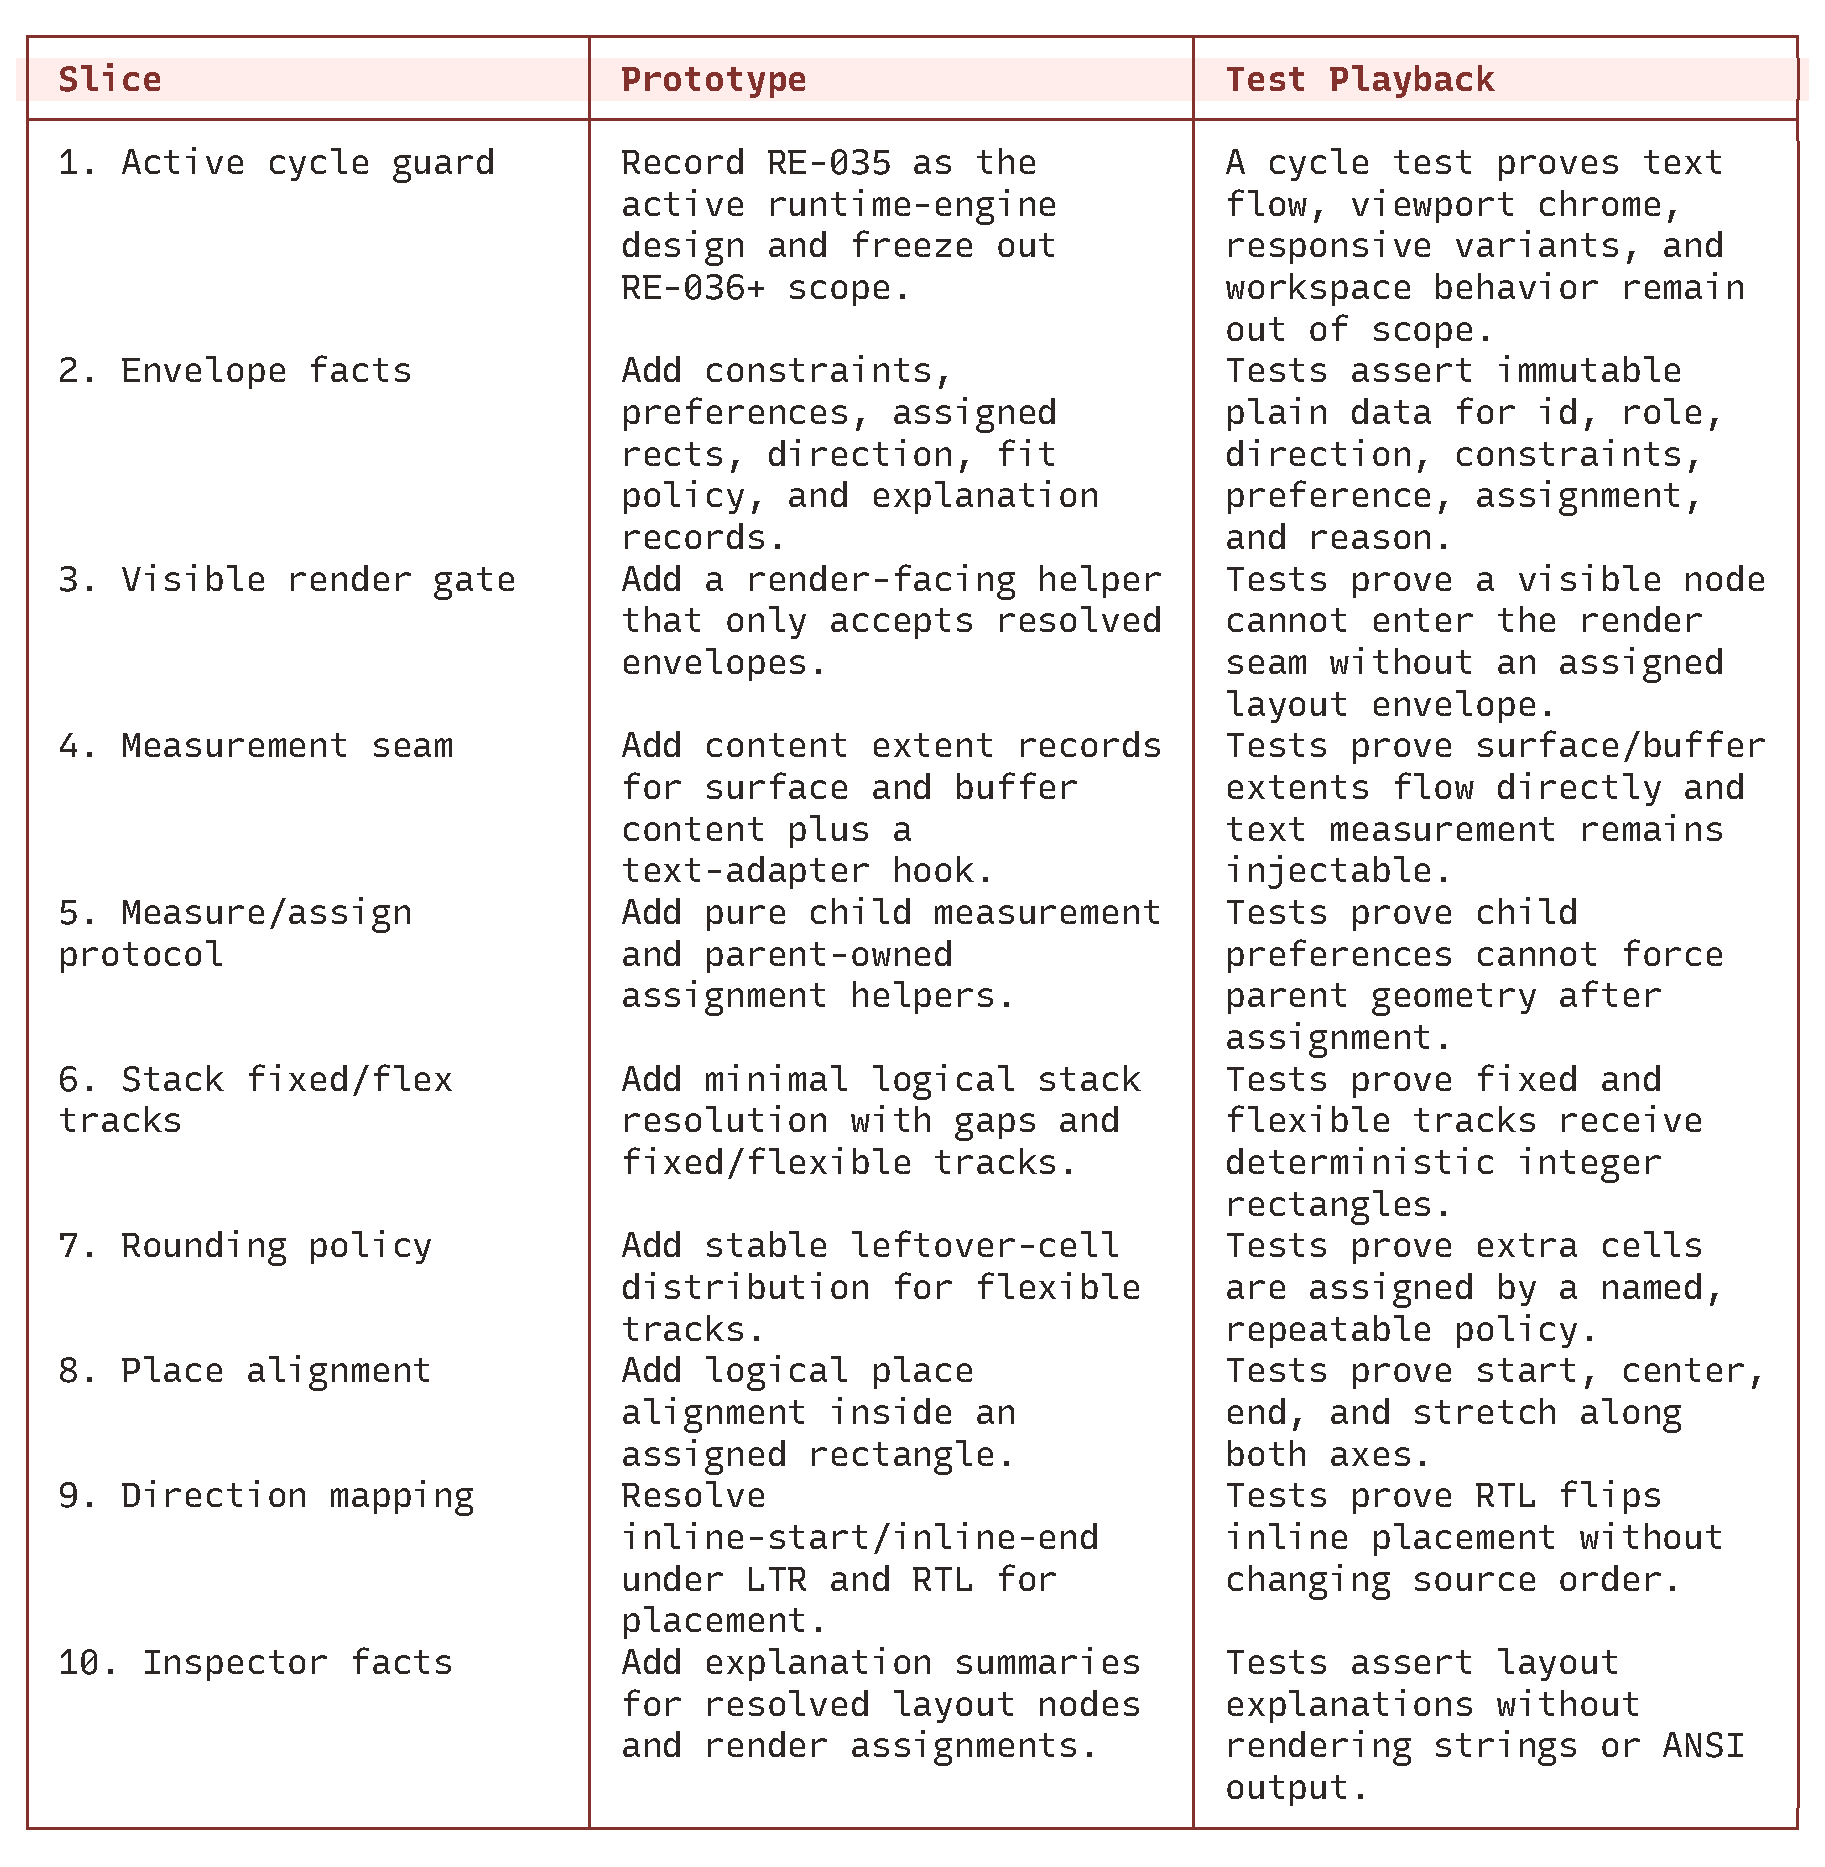
\includegraphics[width=\linewidth]{figures/tables/table-042-g1-1.pdf}
\par\smallskip{\scriptsize\color{BookMuted}Rows 1–10. Actual Bijou table component.}
\end{center}


\subsection{Playback Cadence}\label{record-163-playback-cadence}

\begin{itemize}
\tightlist
\item
  RED: write the slice test first, tied to the playback question above.
\item
  GREEN: add only the pure runtime code needed for that slice.
\item
  LEARN: update this design doc's Drift Check, Playback, and Retrospective when a slice changes the boundary or leaves follow-on debt.
\end{itemize}

\section{Tests To Write First}\label{record-163-tests-to-write-first}

\begin{itemize}
\tightlist
\item
  Cycle test proving RE-035 is the active runtime-engine design and that later text, viewport, chrome, responsive, and workspace work remains out of scope.
\item
  Package-local tests proving visible nodes require a layout envelope before rendering.
\item
  Package-local tests proving child preferences cannot force parent geometry.
\item
  Package-local tests proving stack assigns fixed and flexible tracks deterministically.
\item
  Package-local tests proving leftover cells are rounded by a stable policy.
\item
  Package-local tests proving \texttt{p\allowbreak{}l\allowbreak{}a\allowbreak{}c\allowbreak{}e} aligns children at logical start, center, end, and stretch.
\item
  Package-local tests proving RTL flips inline-start and inline-end placement.
\item
  Package-local tests proving layout explanation facts include node id, role, constraints, preferences, assigned rect, and reason.
\item
  Package-local tests proving a renderer receives the assigned rect from layout resolution.
\end{itemize}

\section{Acceptance Criteria}\label{record-163-acceptance-criteria}

\begin{itemize}
\tightlist
\item
  RED tests fail before implementation and pass after.
\item
  Visible UI nodes cannot enter the render-facing seam without a layout envelope.
\item
  Parent assignment is authoritative and deterministic.
\item
  Stack and place prove the minimum useful layout contract without full flexbox, scrollbars, or workspace behavior.
\item
  Surface and buffer content can report cell extents directly.
\item
  Text measurement remains an adapter seam, not the canonical layout model.
\item
  Layout explanations can be asserted without rendering a string.
\end{itemize}

\section{Risks / Unknowns}\label{record-163-risks-unknowns}

\begin{itemize}
\tightlist
\item
  The first contract may be too small for later viewport or workspace needs, so the types should stay extensible without accepting solver complexity.
\item
  Text measurement is the next hard problem, but it should not drag RE-035 into grapheme, bidi, and cursor-map work.
\item
  Existing string-returning component APIs may need compatibility wrappers while the retained layout path matures.
\item
  Mermaid diagrams in editor tooling can drift, so diagrams should stay conceptual and not become implementation specs.
\end{itemize}

\section{Future Sequence}\label{record-163-future-sequence}

RE-035 deliberately ships the floor, not the full system.

Follow-on cycles should stay layered:

\begin{itemize}
\tightlist
\item
  RE-036 Text Measurement And Inline Flow
\item
  RE-037 Overflow, Viewports, Scroll Anchoring, And Scrollbars
\item
  RE-038 Box Model, Chrome Regions, Hit Testing, And Focus Maps
\item
  RE-039 Responsive Variants, Compression, And Constraint Fallbacks
\item
  RE-040 Mode Lowering And Accessible Layout Semantics
\item
  WS-001 Workspace Tree: Panels, Tabsets, Docks, Drawers
\item
  WS-002 Workspace Interaction: Resize, Drag/Drop, Persistence
\end{itemize}

Workspace features compile into layout. Interaction emits commands. Rendering paints resolved rectangles. None of those layers should mutate layout geometry behind the layout engine's back.

\section{Drift Check}\label{record-163-drift-check}

Started on 2026-06-02 as a pure \texttt{@\allowbreak{}f\allowbreak{}l\allowbreak{}y\allowbreak{}i\allowbreak{}n\allowbreak{}g\allowbreak{}r\allowbreak{}o\allowbreak{}b\allowbreak{}o\allowbreak{}t\allowbreak{}s\allowbreak{}/\allowbreak{}b\allowbreak{}i\allowbreak{}j\allowbreak{}o\allowbreak{}u} core layout slice.

The first ten slices intentionally landed in \texttt{p\allowbreak{}a\allowbreak{}c\allowbreak{}k\allowbreak{}a\allowbreak{}g\allowbreak{}e\allowbreak{}s\allowbreak{}/\allowbreak{}b\allowbreak{}i\allowbreak{}j\allowbreak{}o\allowbreak{}u\allowbreak{}/\allowbreak{}s\allowbreak{}r\allowbreak{}c\allowbreak{}/\allowbreak{}c\allowbreak{}o\allowbreak{}r\allowbreak{}e\allowbreak{}/\allowbreak{}l\allowbreak{}a\allowbreak{}y\allowbreak{}o\allowbreak{}u\allowbreak{}t\allowbreak{}/} instead of \texttt{b\allowbreak{}i\allowbreak{}j\allowbreak{}o\allowbreak{}u\allowbreak{}-\allowbreak{}t\allowbreak{}u\allowbreak{}i}, DOGFOOD, or shell renderers. That keeps the contract mode-neutral and lets tests assert layout truth before any renderer paints.

Confirmed scope boundaries:

\begin{itemize}
\tightlist
\item
  stack and place are proof containers, not a full flexbox or workspace model
\item
  text content uses an injected measurement adapter, not JavaScript string length
\item
  render-facing code receives assigned rectangles through a seam, but existing components are not migrated in this slice
\item
  layout explanation facts are plain data and do not require ANSI output
\end{itemize}

\section{Playback}\label{record-163-playback}

RED:

\begin{itemize}
\tightlist
\item
  Added \texttt{p\allowbreak{}a\allowbreak{}c\allowbreak{}k\allowbreak{}a\allowbreak{}g\allowbreak{}e\allowbreak{}s\allowbreak{}/\allowbreak{}b\allowbreak{}i\allowbreak{}j\allowbreak{}o\allowbreak{}u\allowbreak{}/\allowbreak{}s\allowbreak{}r\allowbreak{}c\allowbreak{}/\allowbreak{}c\allowbreak{}o\allowbreak{}r\allowbreak{}e\allowbreak{}/\allowbreak{}l\allowbreak{}a\allowbreak{}y\allowbreak{}o\allowbreak{}u\allowbreak{}t\allowbreak{}/\allowbreak{}e\allowbreak{}n\allowbreak{}v\allowbreak{}e\allowbreak{}l\allowbreak{}o\allowbreak{}p\allowbreak{}e\allowbreak{}.\allowbreak{}t\allowbreak{}e\allowbreak{}s\allowbreak{}t\allowbreak{}.\allowbreak{}t\allowbreak{}s} before the module existed. The focused test failed because \texttt{.\allowbreak{}/\allowbreak{}e\allowbreak{}n\allowbreak{}v\allowbreak{}e\allowbreak{}l\allowbreak{}o\allowbreak{}p\allowbreak{}e\allowbreak{}.\allowbreak{}j\allowbreak{}s} was missing.
\end{itemize}

GREEN:

\begin{itemize}
\tightlist
\item
  Added immutable layout constraints, preferences, assigned rectangles, directions, fit policy, and resolved-envelope facts.
\item
  Added a render-facing seam that rejects unresolved visible nodes and passes parent-assigned rectangles to the renderer callback.
\item
  Added surface and buffer cell extent helpers plus an injected text measurement seam.
\item
  Added parent-owned child assignment, minimal stack fixed/flex layout, source-order largest-remainder rounding, place alignment, RTL inline start/end mapping, and inspectable explanation facts.
\item
  Exported the RE-035 primitives from \texttt{@\allowbreak{}f\allowbreak{}l\allowbreak{}y\allowbreak{}i\allowbreak{}n\allowbreak{}g\allowbreak{}r\allowbreak{}o\allowbreak{}b\allowbreak{}o\allowbreak{}t\allowbreak{}s\allowbreak{}/\allowbreak{}b\allowbreak{}i\allowbreak{}j\allowbreak{}o\allowbreak{}u}.
\end{itemize}

\section{Retrospective}\label{record-163-retrospective}

The first ten slices establish the boring floor: visible layout facts can now exist and be tested before rendering. The main restraint was keeping RE-035 from turning into RE-036 through RE-040. The current module deliberately does not solve text flow, overflow, hit testing, responsive fallbacks, accessible layout lowering, or workspace behavior.

Follow-on adoption should be separate and test-led: migrate one render-facing surface family at a time to consume assigned rectangles, then introduce text measurement, viewport overflow, and hit-test facts as their own cycles.

%
\chapter{RE-036 Packed Bijou Cells Surface Adapter}\label{record-164}

\noindent{\footnotesize\color{BookMuted}\path{docs/design/RE-036-packed-bijou-cells-surface-adapter.md}\par}\smallskip

\begin{RecordMeta}
title: RE-036 Packed Bijou Cells Surface Adapter
legend: RE
lane: release
priority: high
github_issue: 459
parent_issue: 457
status: complete
keywords:
  - runtime-engine
  - visor
  - packed-cells
  - surface
  - receipts
  - validation
  - v8.0.0

\end{RecordMeta}

Legend: \href{https://github.com/flyingrobots/bijou/blob/1853ad902f6bf219326409e7f743a5a1d6517dbc/docs/legends/RE-runtime-engine.md}{RE - Runtime Engine}

\section{Linked Work}\label{record-164-linked-work}

\begin{itemize}
\tightlist
\item
  User story: \href{https://github.com/flyingrobots/bijou/issues/459}{\#459}
\item
  V8 tracker: \href{https://github.com/flyingrobots/bijou/issues/457}{\#457}
\item
  Broad source lineage: \href{https://github.com/flyingrobots/bijou/issues/302}{\#302}
\item
  Landed artifact-bundle proof: \href{https://github.com/flyingrobots/bijou/issues/458}{\#458}
\item
  V8 contract design: \href{https://github.com/flyingrobots/bijou/blob/cbd70612140e7a450d764b3c7be1c6af878b99bc/docs/design/DX-048-v8-runtime-graph-scene-ir-contract.md}{DX-048 V8 Runtime Graph And Scene IR Contract}
\item
  Artifact-bundle design: \href{https://github.com/flyingrobots/bijou/blob/cbd70612140e7a450d764b3c7be1c6af878b99bc/docs/design/DX-049-visor-artifact-bundle-proof.md}{DX-049 VISOR Artifact Bundle Proof}
\item
  VISOR coordination tracker: \href{https://github.com/flyingrobots/visor/issues/1}{flyingrobots/visor\#1}
\end{itemize}

\section{Decision Summary}\label{record-164-decision-summary}

Bijou will define \texttt{p\allowbreak{}a\allowbreak{}c\allowbreak{}k\allowbreak{}e\allowbreak{}d\allowbreak{}-\allowbreak{}b\allowbreak{}i\allowbreak{}j\allowbreak{}o\allowbreak{}u\allowbreak{}-\allowbreak{}c\allowbreak{}e\allowbreak{}l\allowbreak{}l\allowbreak{}s\allowbreak{}/\allowbreak{}1} as a JSON-shaped terminal receipt whose cell bytes use Bijou's existing ten-byte little-endian packed-cell format, identified as \texttt{b\allowbreak{}i\allowbreak{}j\allowbreak{}o\allowbreak{}u\allowbreak{}-\allowbreak{}p\allowbreak{}a\allowbreak{}c\allowbreak{}k\allowbreak{}e\allowbreak{}d\allowbreak{}-\allowbreak{}c\allowbreak{}e\allowbreak{}l\allowbreak{}l\allowbreak{}-\allowbreak{}u\allowbreak{}8\allowbreak{}x\allowbreak{}1\allowbreak{}0\allowbreak{}-\allowbreak{}l\allowbreak{}e\allowbreak{}/\allowbreak{}1}. Glyphs use the \texttt{u\allowbreak{}n\allowbreak{}i\allowbreak{}c\allowbreak{}o\allowbreak{}d\allowbreak{}e\allowbreak{}-\allowbreak{}g\allowbreak{}r\allowbreak{}a\allowbreak{}p\allowbreak{}h\allowbreak{}e\allowbreak{}m\allowbreak{}e\allowbreak{}-\allowbreak{}s\allowbreak{}i\allowbreak{}d\allowbreak{}e\allowbreak{}-\allowbreak{}t\allowbreak{}a\allowbreak{}b\allowbreak{}l\allowbreak{}e\allowbreak{}/\allowbreak{}1} policy. The receipt carries exact dimensions, bytes, grapheme side-table entries, scene-node provenance, focus facts, and chroma policy facts. A public validator rejects malformed or non-canonical receipts before any \texttt{S\allowbreak{}u\allowbreak{}r\allowbreak{}f\allowbreak{}a\allowbreak{}c\allowbreak{}e} constructor or renderer can sanitize them.

The adapter validates first, creates a packed Bijou \texttt{S\allowbreak{}u\allowbreak{}r\allowbreak{}f\allowbreak{}a\allowbreak{}c\allowbreak{}e}, copies the validated bytes and side table without re-encoding cells, and marks the resulting surface dirty. A successful adaptation therefore preserves the receipt's byte sequence and side-table order exactly. It does not reinterpret the receipt through \texttt{C\allowbreak{}e\allowbreak{}l\allowbreak{}l} objects.

\section{Current Truth}\label{record-164-current-truth}

Bijou already owns a packed terminal \texttt{S\allowbreak{}u\allowbreak{}r\allowbreak{}f\allowbreak{}a\allowbreak{}c\allowbreak{}e}:

\begin{itemize}
\tightlist
\item
  every cell occupies \texttt{1\allowbreak{}0} bytes
\item
  character identity is a little-endian unsigned 16-bit value
\item
  direct character values below \texttt{0\allowbreak{}x\allowbreak{}F\allowbreak{}0\allowbreak{}0\allowbreak{}0} represent BMP code points
\item
  values at or above \texttt{0\allowbreak{}x\allowbreak{}F\allowbreak{}0\allowbreak{}0\allowbreak{}0} index a grapheme side table
\item
  foreground and background colors occupy three unsigned 8-bit channels each
\item
  the flags byte records modifiers and the empty-cell bit
\item
  the alpha byte records six-bit opacity plus foreground/background presence bits
\end{itemize}

The internal \texttt{c\allowbreak{}r\allowbreak{}e\allowbreak{}a\allowbreak{}t\allowbreak{}e\allowbreak{}S\allowbreak{}u\allowbreak{}r\allowbreak{}f\allowbreak{}a\allowbreak{}c\allowbreak{}e\allowbreak{}(\allowbreak{})} boundary sanitizes dimensions. The internal \texttt{d\allowbreak{}e\allowbreak{}c\allowbreak{}o\allowbreak{}d\allowbreak{}e\allowbreak{}C\allowbreak{}h\allowbreak{}a\allowbreak{}r\allowbreak{}(\allowbreak{})} boundary substitutes a space when a side-table reference is missing. Those behaviors are appropriate defensive fallbacks inside the renderer, but they are not valid receipt verification. RE-036 must reject the input before either fallback can hide a malformed external artifact.

DX-048 requires packed cells to map back to scene nodes. \#459 also requires focus and chroma metadata to be validated. The existing packed buffer does not carry those facts, so the receipt must carry them beside the byte payload.

\section{Sponsor Human}\label{record-164-sponsor-human}

A maintainer wants to inspect one portable terminal receipt, see the exact scene, cell, glyph, color, focus, and provenance facts it claims, and adapt it into a Bijou \texttt{S\allowbreak{}u\allowbreak{}r\allowbreak{}f\allowbreak{}a\allowbreak{}c\allowbreak{}e} without wondering whether the adapter repaired the input.

\section{Sponsor Agent}\label{record-164-sponsor-agent}

An agent wants deterministic typed diagnostics for every invalid receipt path and a byte-exact success path it can verify without rendering a live terminal, scraping text, or depending on process-local state.

\section{Hill}\label{record-164-hill}

Given a checked-in \texttt{p\allowbreak{}a\allowbreak{}c\allowbreak{}k\allowbreak{}e\allowbreak{}d\allowbreak{}-\allowbreak{}b\allowbreak{}i\allowbreak{}j\allowbreak{}o\allowbreak{}u\allowbreak{}-\allowbreak{}c\allowbreak{}e\allowbreak{}l\allowbreak{}l\allowbreak{}s\allowbreak{}/\allowbreak{}1} fixture, Bijou can fail closed on invalid shape, dimensions, bytes, glyphs, colors, scene provenance, focus, or chroma metadata, then adapt a valid receipt into a packed \texttt{S\allowbreak{}u\allowbreak{}r\allowbreak{}f\allowbreak{}a\allowbreak{}c\allowbreak{}e} whose dimensions, buffer bytes, side-table order, decoded cells, and scene ownership remain inspectable and deterministic.

\section{Playback Questions}\label{record-164-playback-questions}

\begin{itemize}
\tightlist
\item
  Which exact packed-cell version and cell format does the receipt use?
\item
  How many cells and bytes does the receipt claim?
\item
  Which scene and scene nodes own each packed cell?
\item
  Which side-table entry supplies each non-direct glyph?
\item
  Which node is focused, and which nodes are focusable?
\item
  Which color space, channel encoding, alpha encoding, and terminal-default policy govern the bytes?
\item
  Can malformed dimensions, colors, glyph references, focus facts, or scene mappings reach \texttt{c\allowbreak{}r\allowbreak{}e\allowbreak{}a\allowbreak{}t\allowbreak{}e\allowbreak{}S\allowbreak{}u\allowbreak{}r\allowbreak{}f\allowbreak{}a\allowbreak{}c\allowbreak{}e\allowbreak{}(\allowbreak{})}?
\item
  Does adaptation preserve every byte and side-table entry without normalization?
\end{itemize}

\section{Scope}\label{record-164-scope}

\begin{itemize}
\tightlist
\item
  Define the public \texttt{p\allowbreak{}a\allowbreak{}c\allowbreak{}k\allowbreak{}e\allowbreak{}d\allowbreak{}-\allowbreak{}b\allowbreak{}i\allowbreak{}j\allowbreak{}o\allowbreak{}u\allowbreak{}-\allowbreak{}c\allowbreak{}e\allowbreak{}l\allowbreak{}l\allowbreak{}s\allowbreak{}/\allowbreak{}1} receipt type and version constants.
\item
  Define a typed deterministic validation error with stable code and path.
\item
  Validate the receipt's exact object shape and nested metadata shapes.
\item
  Validate dimensions, cell count, stride, byte count, and byte values.
\item
  Validate direct glyph values and side-table references.
\item
  Validate canonical side-table entries and reference coverage.
\item
  Validate foreground/background presence-bit color semantics.
\item
  Validate scene-node provenance for every cell.
\item
  Validate focus and chroma metadata.
\item
  Adapt a valid receipt into Bijou's existing packed \texttt{S\allowbreak{}u\allowbreak{}r\allowbreak{}f\allowbreak{}a\allowbreak{}c\allowbreak{}e}.
\item
  Prove byte-exact and side-table-exact adaptation with a checked-in fixture.
\item
  Export the contract, validator, error, and adapter through the public Bijou package surface.
\end{itemize}

\section{Non-Goals}\label{record-164-non-goals}

This cycle does not:

\begin{itemize}
\tightlist
\item
  change Bijou's existing packed-cell byte format
\item
  make Geordi a Bijou dependency
\item
  implement a Geordi packed-cell renderer
\item
  implement terminal frame capture, replay, streaming, or compression
\item
  define VISOR storage or indexing behavior
\item
  add browser, WebGPU, image, shader, raster, or native-render targets
\item
  normalize invalid receipts into accepted ones
\item
  infer scene ownership from geometry after receipt creation
\item
  validate an entire \texttt{u\allowbreak{}i\allowbreak{}-\allowbreak{}s\allowbreak{}c\allowbreak{}e\allowbreak{}n\allowbreak{}e\allowbreak{}-\allowbreak{}i\allowbreak{}r\allowbreak{}/\allowbreak{}1} artifact against the declared scene hash
\item
  redesign \texttt{S\allowbreak{}u\allowbreak{}r\allowbreak{}f\allowbreak{}a\allowbreak{}c\allowbreak{}e}, \texttt{C\allowbreak{}e\allowbreak{}l\allowbreak{}l}, or terminal diff rendering
\item
  expand \#459 into the remaining \#302 or \#457 tracker scope
\end{itemize}

\section{Receipt Contract}\label{record-164-receipt-contract}

The public receipt shape is:

\begin{CodeBlock}
interface PackedBijouCellsReceipt {
  readonly receiptVersion: 'packed-bijou-cells/1';
  readonly widthCells: number;
  readonly heightCells: number;
  readonly cellFormatId: 'bijou-packed-cell-u8x10-le/1';
  readonly glyphPolicyId: 'unicode-grapheme-side-table/1';
  readonly bytes: readonly number[];
  readonly sideTable: readonly string[];
  readonly scene: {
    readonly sceneVersion: 'ui-scene-ir/1';
    readonly sceneHash: string;
    readonly nodeIds: readonly string[];
    readonly cellNodeIds: readonly string[];
  };
  readonly focus: {
    readonly focusedNodeId: string | null;
    readonly focusableNodeIds: readonly string[];
  };
  readonly chroma: {
    readonly colorSpace: 'srgb';
    readonly channelEncoding: 'uint8';
    readonly alphaEncoding: 'uint6';
    readonly terminalDefaultEncoding: 'presence-bits';
  };
}
\end{CodeBlock}

The receipt is JSON-shaped. It does not carry \texttt{U\allowbreak{}i\allowbreak{}n\allowbreak{}t\allowbreak{}8\allowbreak{}A\allowbreak{}r\allowbreak{}r\allowbreak{}a\allowbreak{}y}, \texttt{S\allowbreak{}e\allowbreak{}t}, \texttt{M\allowbreak{}a\allowbreak{}p}, functions, symbols, absolute paths, timestamps, process identifiers, terminal handles, or mutable renderer objects.

\section{Dimension And Byte Laws}\label{record-164-dimension-and-byte-laws}

\begin{itemize}
\tightlist
\item
  \texttt{w\allowbreak{}i\allowbreak{}d\allowbreak{}t\allowbreak{}h\allowbreak{}C\allowbreak{}e\allowbreak{}l\allowbreak{}l\allowbreak{}s} and \texttt{h\allowbreak{}e\allowbreak{}i\allowbreak{}g\allowbreak{}h\allowbreak{}t\allowbreak{}C\allowbreak{}e\allowbreak{}l\allowbreak{}l\allowbreak{}s} are positive safe integers.
\item
  neither dimension exceeds the renderer's \texttt{9\allowbreak{},\allowbreak{}9\allowbreak{}9\allowbreak{}9}-cell cursor-coordinate limit.
\item
  \texttt{w\allowbreak{}i\allowbreak{}d\allowbreak{}t\allowbreak{}h\allowbreak{}C\allowbreak{}e\allowbreak{}l\allowbreak{}l\allowbreak{}s\allowbreak{} \allowbreak{}*\allowbreak{} \allowbreak{}h\allowbreak{}e\allowbreak{}i\allowbreak{}g\allowbreak{}h\allowbreak{}t\allowbreak{}C\allowbreak{}e\allowbreak{}l\allowbreak{}l\allowbreak{}s} is a safe integer.
\item
  the receipt contains at most \texttt{1\allowbreak{}0\allowbreak{}0\allowbreak{},\allowbreak{}0\allowbreak{}0\allowbreak{}0} cells.
\item
  \texttt{c\allowbreak{}e\allowbreak{}l\allowbreak{}l\allowbreak{}C\allowbreak{}o\allowbreak{}u\allowbreak{}n\allowbreak{}t\allowbreak{} \allowbreak{}*\allowbreak{} \allowbreak{}1\allowbreak{}0} is a safe integer.
\item
  \texttt{b\allowbreak{}y\allowbreak{}t\allowbreak{}e\allowbreak{}s\allowbreak{}.\allowbreak{}l\allowbreak{}e\allowbreak{}n\allowbreak{}g\allowbreak{}t\allowbreak{}h} equals \texttt{c\allowbreak{}e\allowbreak{}l\allowbreak{}l\allowbreak{}C\allowbreak{}o\allowbreak{}u\allowbreak{}n\allowbreak{}t\allowbreak{} \allowbreak{}*\allowbreak{} \allowbreak{}1\allowbreak{}0}.
\item
  every byte is a canonical integer in the inclusive range \texttt{0} through \texttt{2\allowbreak{}5\allowbreak{}5}; negative zero is rejected
\item
  \texttt{c\allowbreak{}e\allowbreak{}l\allowbreak{}l\allowbreak{}F\allowbreak{}o\allowbreak{}r\allowbreak{}m\allowbreak{}a\allowbreak{}t\allowbreak{}I\allowbreak{}d} fixes the stride at \texttt{1\allowbreak{}0}; no receipt-defined stride exists
\end{itemize}

The validator checks those laws before calling \texttt{c\allowbreak{}r\allowbreak{}e\allowbreak{}a\allowbreak{}t\allowbreak{}e\allowbreak{}S\allowbreak{}u\allowbreak{}r\allowbreak{}f\allowbreak{}a\allowbreak{}c\allowbreak{}e\allowbreak{}(\allowbreak{})}. Zero, negative, fractional, infinite, \texttt{N\allowbreak{}a\allowbreak{}N}, unsafe, overflowing, excessive, or byte-length-mismatched dimensions fail.

\section{Glyph Laws}\label{record-164-glyph-laws}

\begin{itemize}
\tightlist
\item
  the character value is decoded from byte offsets \texttt{0} and \texttt{1} as unsigned 16-bit little-endian
\item
  direct value \texttt{0} is rejected; an empty cell uses a space glyph plus the empty-cell flag
\item
  direct values below \texttt{0\allowbreak{}x\allowbreak{}F\allowbreak{}0\allowbreak{}0\allowbreak{}0} must not be UTF-16 surrogate code points
\item
  direct values are terminal-control safe graphemes of width \texttt{1}
\item
  values at or above \texttt{0\allowbreak{}x\allowbreak{}F\allowbreak{}0\allowbreak{}0\allowbreak{}0} must reference an existing side-table entry
\item
  every side-table entry is non-empty, terminal-control safe, and exactly one grapheme with terminal width \texttt{1}
\item
  format-control, mark-only, and default-ignorable-only graphemes are rejected
\item
  every side-table entry contains at most \texttt{2\allowbreak{}5\allowbreak{}6} UTF-16 code units and \texttt{3\allowbreak{}2} UTF-8 bytes
\item
  directly encodable values below \texttt{0\allowbreak{}x\allowbreak{}F\allowbreak{}0\allowbreak{}0\allowbreak{}0} are not valid side-table entries
\item
  side-table entries are unique
\item
  every side-table entry is referenced by at least one cell
\item
  side-table order is authoritative and is never sorted, deduplicated, or reconstructed by the adapter
\end{itemize}

Rejecting unreferenced entries makes the receipt canonical and prevents multiple byte-equivalent receipts from carrying arbitrary unused glyph data.

\section{Color And Modifier Laws}\label{record-164-color-and-modifier-laws}

The six color-channel bytes are always unsigned 8-bit values by the byte law. The alpha byte's low six bits encode opacity. Bit \texttt{6} records foreground presence and bit \texttt{7} records background presence.

\begin{itemize}
\tightlist
\item
  when the foreground presence bit is unset, all three foreground channels are \texttt{0}
\item
  when the background presence bit is unset, all three background channels are \texttt{0}
\item
  an absent color means terminal default; it does not mean black
\item
  the dashed modifier flag is valid only with the dotted/dashed underline value
\item
  all other modifier and empty-cell bits retain their existing Bijou meaning
\end{itemize}

The adapter copies those bytes. It does not synthesize terminal defaults, resolve theme tokens, quantize colors, or reconstruct modifier lists.

\section{Scene And Focus Laws}\label{record-164-scene-and-focus-laws}

\begin{itemize}
\tightlist
\item
  \texttt{s\allowbreak{}c\allowbreak{}e\allowbreak{}n\allowbreak{}e\allowbreak{}.\allowbreak{}s\allowbreak{}c\allowbreak{}e\allowbreak{}n\allowbreak{}e\allowbreak{}V\allowbreak{}e\allowbreak{}r\allowbreak{}s\allowbreak{}i\allowbreak{}o\allowbreak{}n} is exactly \texttt{u\allowbreak{}i\allowbreak{}-\allowbreak{}s\allowbreak{}c\allowbreak{}e\allowbreak{}n\allowbreak{}e\allowbreak{}-\allowbreak{}i\allowbreak{}r\allowbreak{}/\allowbreak{}1}
\item
  \texttt{s\allowbreak{}c\allowbreak{}e\allowbreak{}n\allowbreak{}e\allowbreak{}.\allowbreak{}s\allowbreak{}c\allowbreak{}e\allowbreak{}n\allowbreak{}e\allowbreak{}H\allowbreak{}a\allowbreak{}s\allowbreak{}h} is a lowercase 64-character SHA-256 hexadecimal digest
\item
  \texttt{s\allowbreak{}c\allowbreak{}e\allowbreak{}n\allowbreak{}e\allowbreak{}.\allowbreak{}n\allowbreak{}o\allowbreak{}d\allowbreak{}e\allowbreak{}I\allowbreak{}d\allowbreak{}s} is non-empty, unique, and contains canonical non-empty ids
\item
  \texttt{s\allowbreak{}c\allowbreak{}e\allowbreak{}n\allowbreak{}e\allowbreak{}.\allowbreak{}c\allowbreak{}e\allowbreak{}l\allowbreak{}l\allowbreak{}N\allowbreak{}o\allowbreak{}d\allowbreak{}e\allowbreak{}I\allowbreak{}d\allowbreak{}s\allowbreak{}.\allowbreak{}l\allowbreak{}e\allowbreak{}n\allowbreak{}g\allowbreak{}t\allowbreak{}h} equals the cell count
\item
  every cell node id occurs in \texttt{s\allowbreak{}c\allowbreak{}e\allowbreak{}n\allowbreak{}e\allowbreak{}.\allowbreak{}n\allowbreak{}o\allowbreak{}d\allowbreak{}e\allowbreak{}I\allowbreak{}d\allowbreak{}s}
\item
  \texttt{f\allowbreak{}o\allowbreak{}c\allowbreak{}u\allowbreak{}s\allowbreak{}.\allowbreak{}f\allowbreak{}o\allowbreak{}c\allowbreak{}u\allowbreak{}s\allowbreak{}a\allowbreak{}b\allowbreak{}l\allowbreak{}e\allowbreak{}N\allowbreak{}o\allowbreak{}d\allowbreak{}e\allowbreak{}I\allowbreak{}d\allowbreak{}s} is unique
\item
  every focusable node id occurs in \texttt{s\allowbreak{}c\allowbreak{}e\allowbreak{}n\allowbreak{}e\allowbreak{}.\allowbreak{}n\allowbreak{}o\allowbreak{}d\allowbreak{}e\allowbreak{}I\allowbreak{}d\allowbreak{}s}
\item
  \texttt{f\allowbreak{}o\allowbreak{}c\allowbreak{}u\allowbreak{}s\allowbreak{}.\allowbreak{}f\allowbreak{}o\allowbreak{}c\allowbreak{}u\allowbreak{}s\allowbreak{}e\allowbreak{}d\allowbreak{}N\allowbreak{}o\allowbreak{}d\allowbreak{}e\allowbreak{}I\allowbreak{}d} is either \texttt{n\allowbreak{}u\allowbreak{}l\allowbreak{}l} or occurs in \texttt{f\allowbreak{}o\allowbreak{}c\allowbreak{}u\allowbreak{}s\allowbreak{}.\allowbreak{}f\allowbreak{}o\allowbreak{}c\allowbreak{}u\allowbreak{}s\allowbreak{}a\allowbreak{}b\allowbreak{}l\allowbreak{}e\allowbreak{}N\allowbreak{}o\allowbreak{}d\allowbreak{}e\allowbreak{}I\allowbreak{}d\allowbreak{}s}
\end{itemize}

Every cell has an owning scene node. Background, empty, or padding cells must name the scene node that intentionally emitted them; \texttt{n\allowbreak{}u\allowbreak{}l\allowbreak{}l} ownership is not accepted.

\section{Chroma Laws}\label{record-164-chroma-laws}

The first receipt version supports one explicit chroma profile:

\begin{CodeBlock}
colorSpace: srgb
channelEncoding: uint8
alphaEncoding: uint6
terminalDefaultEncoding: presence-bits
\end{CodeBlock}

All four fields are mandatory and exact. Supporting another color space, channel width, alpha encoding, or terminal-default policy requires a new declared receipt or cell-format version. The validator does not silently convert unsupported metadata.

\section{Validation Error Contract}\label{record-164-validation-error-contract}

Invalid input throws \texttt{P\allowbreak{}a\allowbreak{}c\allowbreak{}k\allowbreak{}e\allowbreak{}d\allowbreak{}B\allowbreak{}i\allowbreak{}j\allowbreak{}o\allowbreak{}u\allowbreak{}C\allowbreak{}e\allowbreak{}l\allowbreak{}l\allowbreak{}s\allowbreak{}V\allowbreak{}a\allowbreak{}l\allowbreak{}i\allowbreak{}d\allowbreak{}a\allowbreak{}t\allowbreak{}i\allowbreak{}o\allowbreak{}n\allowbreak{}E\allowbreak{}r\allowbreak{}r\allowbreak{}o\allowbreak{}r} with:

\begin{CodeBlock}
interface PackedBijouCellsValidationErrorShape {
  readonly code: PackedBijouCellsValidationCode;
  readonly path: string;
  readonly detail: string;
}
\end{CodeBlock}

The message format is deterministic:

\begin{CodeBlock}
packed-bijou-cells/1 <code> at <path>: <detail>
\end{CodeBlock}

Codes distinguish invalid shape, unknown field, wrong literal, invalid dimension, invalid byte, byte-length mismatch, invalid glyph, invalid color, invalid modifier, invalid scene mapping, invalid focus, and invalid chroma. Paths use JSON-compatible segments such as \texttt{\$\allowbreak{}.\allowbreak{}b\allowbreak{}y\allowbreak{}t\allowbreak{}e\allowbreak{}s\allowbreak{}[\allowbreak{}1\allowbreak{}7\allowbreak{}]} and \texttt{\$\allowbreak{}.\allowbreak{}f\allowbreak{}o\allowbreak{}c\allowbreak{}u\allowbreak{}s\allowbreak{}.\allowbreak{}f\allowbreak{}o\allowbreak{}c\allowbreak{}u\allowbreak{}s\allowbreak{}e\allowbreak{}d\allowbreak{}N\allowbreak{}o\allowbreak{}d\allowbreak{}e\allowbreak{}I\allowbreak{}d}. Control and default-ignorable characters are escaped as Unicode escape sequences before entering a diagnostic path.

Validation returns a fresh receipt value only after the entire object passes. No partial receipt or partially created \texttt{S\allowbreak{}u\allowbreak{}r\allowbreak{}f\allowbreak{}a\allowbreak{}c\allowbreak{}e} escapes a failure.

\section{Surface Adapter Contract}\label{record-164-surface-adapter-contract}

\texttt{a\allowbreak{}d\allowbreak{}a\allowbreak{}p\allowbreak{}t\allowbreak{}P\allowbreak{}a\allowbreak{}c\allowbreak{}k\allowbreak{}e\allowbreak{}d\allowbreak{}B\allowbreak{}i\allowbreak{}j\allowbreak{}o\allowbreak{}u\allowbreak{}C\allowbreak{}e\allowbreak{}l\allowbreak{}l\allowbreak{}s\allowbreak{}T\allowbreak{}o\allowbreak{}S\allowbreak{}u\allowbreak{}r\allowbreak{}f\allowbreak{}a\allowbreak{}c\allowbreak{}e\allowbreak{}(\allowbreak{}i\allowbreak{}n\allowbreak{}p\allowbreak{}u\allowbreak{}t\allowbreak{})} performs this sequence:

\begin{enumerate}
\def\labelenumi{\arabic{enumi}.}
\tightlist
\item
  Parse and validate the unknown input.
\item
  Create a packed \texttt{S\allowbreak{}u\allowbreak{}r\allowbreak{}f\allowbreak{}a\allowbreak{}c\allowbreak{}e} with the validated positive dimensions.
\item
  Copy the validated bytes into \texttt{s\allowbreak{}u\allowbreak{}r\allowbreak{}f\allowbreak{}a\allowbreak{}c\allowbreak{}e\allowbreak{}.\allowbreak{}b\allowbreak{}u\allowbreak{}f\allowbreak{}f\allowbreak{}e\allowbreak{}r}.
\item
  Copy side-table entries in their declared order.
\item
  Mark all cells dirty for the first terminal render.
\item
  Return the packed \texttt{S\allowbreak{}u\allowbreak{}r\allowbreak{}f\allowbreak{}a\allowbreak{}c\allowbreak{}e}.
\end{enumerate}

The following round-trip assertions are mandatory:

\begin{CodeBlock}
surface.width === receipt.widthCells
surface.height === receipt.heightCells
Array.from(surface.buffer) deep-equals receipt.bytes
surface.sideTable deep-equals receipt.sideTable
\end{CodeBlock}

Decoded cells may be inspected as secondary evidence. Re-encoding decoded \texttt{C\allowbreak{}e\allowbreak{}l\allowbreak{}l} objects is not the adaptation mechanism.

\section{Accessibility And Assistive Posture}\label{record-164-accessibility-and-assistive-posture}

Packed cells are visual terminal output, not an accessibility tree. The receipt preserves scene-node and focus identity so a later inspector can link the visual proof back to semantic roles and accessible names in \texttt{u\allowbreak{}i\allowbreak{}-\allowbreak{}s\allowbreak{}c\allowbreak{}e\allowbreak{}n\allowbreak{}e\allowbreak{}-\allowbreak{}i\allowbreak{}r\allowbreak{}/\allowbreak{}1}. This cycle makes no claim that packed bytes alone provide a screen-reader representation.

The adapter must not erase focus identity or imply that terminal color is the only carrier of meaning. Semantic accessibility remains owned by the source artifact and scene contract.

\section{Localization And Directionality Posture}\label{record-164-localization-and-directionality-posture}

Side-table validation is Unicode-aware and accepts one terminal-width grapheme per entry. This cycle does not implement bidirectional reordering, wide-cell layout, locale-aware shaping, or grapheme fallback. A producer must lower those concerns before emitting this one-cell-per-glyph receipt.

Rejecting control-bearing, multi-grapheme, or non-unit-width entries prevents the adapter from creating a \texttt{S\allowbreak{}u\allowbreak{}r\allowbreak{}f\allowbreak{}a\allowbreak{}c\allowbreak{}e} whose geometry disagrees with the receipt dimensions.

\section{Agent Inspectability And Explainability Posture}\label{record-164-agent-inspectability-and-explainability-posture}

An agent can inspect:

\begin{itemize}
\tightlist
\item
  exact version and policy literals
\item
  dimensions and derived cell count
\item
  exact byte payload
\item
  glyph side table and cell references
\item
  scene hash and node inventory
\item
  per-cell scene ownership
\item
  focus inventory and active focus
\item
  exact chroma profile
\item
  a stable validation code and path for failures
\end{itemize}

No live terminal, component tree, renderer loop, hidden registry, or host state is required to explain success or failure.

\section{Linked Invariants}\label{record-164-linked-invariants}

\begin{itemize}
\tightlist
\item
  \href{https://github.com/flyingrobots/bijou/blob/cbd70612140e7a450d764b3c7be1c6af878b99bc/docs/invariants/buffer-holds-facts.md}{The Buffer Holds Facts}: the receipt is portable data and the adapter preserves its packed facts.
\item
  \href{https://github.com/flyingrobots/bijou/blob/cbd70612140e7a450d764b3c7be1c6af878b99bc/docs/invariants/schemas-live-at-boundaries.md}{Schemas Live At Boundaries}: malformed receipts fail with stable code and path.
\item
  \href{https://github.com/flyingrobots/bijou/blob/cbd70612140e7a450d764b3c7be1c6af878b99bc/docs/invariants/tests-are-the-spec.md}{Tests Are the Spec}: executable fixtures define the accepted receipt and failure behavior.
\item
  \href{https://github.com/flyingrobots/bijou/blob/cbd70612140e7a450d764b3c7be1c6af878b99bc/docs/invariants/host-apis-stay-behind-adapters.md}{Host APIs Stay Behind Adapters}: validation and adaptation require no host, filesystem, process, or network capability.
\end{itemize}

\section{Implementation Outline}\label{record-164-implementation-outline}

\begin{enumerate}
\def\labelenumi{\arabic{enumi}.}
\tightlist
\item
  Synchronize \texttt{R\allowbreak{}O\allowbreak{}A\allowbreak{}D\allowbreak{}M\allowbreak{}A\allowbreak{}P\allowbreak{}.\allowbreak{}m\allowbreak{}d} and \texttt{B\allowbreak{}E\allowbreak{}A\allowbreak{}R\allowbreak{}I\allowbreak{}N\allowbreak{}G\allowbreak{}.\allowbreak{}m\allowbreak{}d} with the landed \#468 proof and active \#459 lane.
\item
  Add this design packet and a design-policy regression test.
\item
  Add a checked-in valid receipt fixture and focused tests that fail because the public validator and adapter do not exist.
\item
  Implement constants, public types, typed errors, exact-shape validation, and canonical field validation.
\item
  Implement glyph, color, scene, focus, and chroma validation.
\item
  Implement the byte-copying packed \texttt{S\allowbreak{}u\allowbreak{}r\allowbreak{}f\allowbreak{}a\allowbreak{}c\allowbreak{}e} adapter.
\item
  Export the public contract through \texttt{@\allowbreak{}f\allowbreak{}l\allowbreak{}y\allowbreak{}i\allowbreak{}n\allowbreak{}g\allowbreak{}r\allowbreak{}o\allowbreak{}b\allowbreak{}o\allowbreak{}t\allowbreak{}s\allowbreak{}/\allowbreak{}b\allowbreak{}i\allowbreak{}j\allowbreak{}o\allowbreak{}u}.
\item
  Update reference documentation, changelog, roadmap evidence, and this design's closeout.
\item
  Run focused tests, package typecheck, lint, Code Dojo gates, docs gates, generators, the full suite, and pre-push verification.
\end{enumerate}

\section{Tests To Write First}\label{record-164-tests-to-write-first}

\begin{itemize}
\tightlist
\item
  A checked-in valid fixture fails to import through the missing public API.
\item
  The valid fixture adapts with exact dimensions, bytes, and side-table order.
\item
  Unknown top-level and nested fields fail.
\item
  Wrong version and policy literals fail.
\item
  Zero, negative, fractional, unsafe, overflowing, and above-\texttt{9\allowbreak{},\allowbreak{}9\allowbreak{}9\allowbreak{}9} dimensions fail.
\item
  Byte-length mismatch and non-byte values fail.
\item
  Missing side-table references fail instead of decoding as spaces.
\item
  Surrogate direct glyph values fail.
\item
  Empty, control-bearing, multi-grapheme, duplicate, wide, and unreferenced side-table entries fail.
\item
  Nonzero RGB channels with an absent color presence bit fail.
\item
  Invalid dashed-modifier combinations fail.
\item
  Duplicate or empty scene-node ids fail.
\item
  Missing and unknown per-cell scene ownership fails.
\item
  Unknown, duplicate, or inconsistent focus ids fail.
\item
  Unsupported chroma values fail without conversion.
\item
  Adaptation never calls a renderer and never re-encodes cells through \texttt{S\allowbreak{}u\allowbreak{}r\allowbreak{}f\allowbreak{}a\allowbreak{}c\allowbreak{}e\allowbreak{}.\allowbreak{}s\allowbreak{}e\allowbreak{}t\allowbreak{}(\allowbreak{})} or \texttt{S\allowbreak{}u\allowbreak{}r\allowbreak{}f\allowbreak{}a\allowbreak{}c\allowbreak{}e\allowbreak{}.\allowbreak{}s\allowbreak{}e\allowbreak{}t\allowbreak{}R\allowbreak{}G\allowbreak{}B\allowbreak{}(\allowbreak{})}.
\end{itemize}

\section{Validation Plan}\label{record-164-validation-plan}

Focused proof:

\begin{CodeBlock}
npx vitest run tests/cycles/RE-036
\end{CodeBlock}

Package and static proof:

\begin{CodeBlock}
npm run typecheck
npm run lint
npm run code-dojo:verify
npm run docs:inventory
git diff --check
\end{CodeBlock}

Full repository proof:

\begin{CodeBlock}
npm run code-dojo:ci
\end{CodeBlock}

If repository script names differ, use the documented owning commands and record the exact successful commands in closeout.

\section{Acceptance Criteria}\label{record-164-acceptance-criteria}

\begin{itemize}
\tightlist
\item
  \texttt{p\allowbreak{}a\allowbreak{}c\allowbreak{}k\allowbreak{}e\allowbreak{}d\allowbreak{}-\allowbreak{}b\allowbreak{}i\allowbreak{}j\allowbreak{}o\allowbreak{}u\allowbreak{}-\allowbreak{}c\allowbreak{}e\allowbreak{}l\allowbreak{}l\allowbreak{}s\allowbreak{}/\allowbreak{}1} is a public documented receipt contract.
\item
  The public validator rejects malformed shape, dimensions, bytes, glyphs, colors, scene mappings, focus facts, and chroma facts deterministically.
\item
  A checked-in fixture adapts into a packed terminal \texttt{S\allowbreak{}u\allowbreak{}r\allowbreak{}f\allowbreak{}a\allowbreak{}c\allowbreak{}e}.
\item
  Adapted dimensions, bytes, and side-table order exactly match the fixture.
\item
  Every receipt cell maps to a declared \texttt{u\allowbreak{}i\allowbreak{}-\allowbreak{}s\allowbreak{}c\allowbreak{}e\allowbreak{}n\allowbreak{}e\allowbreak{}-\allowbreak{}i\allowbreak{}r\allowbreak{}/\allowbreak{}1} node.
\item
  Invalid side-table references never fall through to a replacement space.
\item
  Invalid dimensions never reach dimension sanitation.
\item
  No Geordi, VISOR, host, filesystem, network, or live-terminal dependency is introduced.
\item
  Public types, errors, constants, validator, and adapter are exported.
\item
  Focused and full repository gates pass.
\end{itemize}

\section{Closeout Notes}\label{record-164-closeout-notes}

RE-036 exports \texttt{p\allowbreak{}a\allowbreak{}r\allowbreak{}s\allowbreak{}e\allowbreak{}P\allowbreak{}a\allowbreak{}c\allowbreak{}k\allowbreak{}e\allowbreak{}d\allowbreak{}B\allowbreak{}i\allowbreak{}j\allowbreak{}o\allowbreak{}u\allowbreak{}C\allowbreak{}e\allowbreak{}l\allowbreak{}l\allowbreak{}s\allowbreak{}R\allowbreak{}e\allowbreak{}c\allowbreak{}e\allowbreak{}i\allowbreak{}p\allowbreak{}t\allowbreak{}(\allowbreak{})} and \texttt{a\allowbreak{}d\allowbreak{}a\allowbreak{}p\allowbreak{}t\allowbreak{}P\allowbreak{}a\allowbreak{}c\allowbreak{}k\allowbreak{}e\allowbreak{}d\allowbreak{}B\allowbreak{}i\allowbreak{}j\allowbreak{}o\allowbreak{}u\allowbreak{}C\allowbreak{}e\allowbreak{}l\allowbreak{}l\allowbreak{}s\allowbreak{}T\allowbreak{}o\allowbreak{}S\allowbreak{}u\allowbreak{}r\allowbreak{}f\allowbreak{}a\allowbreak{}c\allowbreak{}e\allowbreak{}(\allowbreak{})} from \texttt{@\allowbreak{}f\allowbreak{}l\allowbreak{}y\allowbreak{}i\allowbreak{}n\allowbreak{}g\allowbreak{}r\allowbreak{}o\allowbreak{}b\allowbreak{}o\allowbreak{}t\allowbreak{}s\allowbreak{}/\allowbreak{}b\allowbreak{}i\allowbreak{}j\allowbreak{}o\allowbreak{}u}. The validator rejects non-plain or inexact JSON shapes, unsafe or excessive dimensions, non-byte payloads, non-canonical glyphs, terminal-default color drift, invalid modifier combinations, incomplete scene ownership, inconsistent focus, and unsupported chroma before surface allocation.

The checked \texttt{2} by \texttt{2} fixture preserves all \texttt{4\allowbreak{}0} bytes and both side-table entries through adaptation. It includes direct, combining, and private-use glyph evidence; explicit and terminal-default colors; per-cell scene ownership; and focus metadata. The adapter copies the payload directly into a packed \texttt{S\allowbreak{}u\allowbreak{}r\allowbreak{}f\allowbreak{}a\allowbreak{}c\allowbreak{}e}, preserves side-table order, and marks every cell dirty without calling \texttt{S\allowbreak{}u\allowbreak{}r\allowbreak{}f\allowbreak{}a\allowbreak{}c\allowbreak{}e\allowbreak{}.\allowbreak{}s\allowbreak{}e\allowbreak{}t\allowbreak{}(\allowbreak{})} or \texttt{S\allowbreak{}u\allowbreak{}r\allowbreak{}f\allowbreak{}a\allowbreak{}c\allowbreak{}e\allowbreak{}.\allowbreak{}s\allowbreak{}e\allowbreak{}t\allowbreak{}R\allowbreak{}G\allowbreak{}B\allowbreak{}(\allowbreak{})}.

Focused RE-036 verification passes \texttt{1\allowbreak{}6} tests across \texttt{5} suites. Full \texttt{n\allowbreak{}p\allowbreak{}m\allowbreak{} \allowbreak{}r\allowbreak{}u\allowbreak{}n\allowbreak{} \allowbreak{}c\allowbreak{}o\allowbreak{}d\allowbreak{}e\allowbreak{}-\allowbreak{}d\allowbreak{}o\allowbreak{}j\allowbreak{}o\allowbreak{}:\allowbreak{}c\allowbreak{}i} verification passes \texttt{4\allowbreak{},\allowbreak{}0\allowbreak{}3\allowbreak{}1} tests across \texttt{8\allowbreak{}9\allowbreak{}1} test files. Code Dojo holds its \texttt{6\allowbreak{}2}-violation aggregate baseline: \texttt{3\allowbreak{}7} file/context, \texttt{2\allowbreak{}5} code-size, \texttt{0} mock-ban, and \texttt{0} ESLint. \texttt{n\allowbreak{}p\allowbreak{}m\allowbreak{} \allowbreak{}r\allowbreak{}u\allowbreak{}n\allowbreak{} \allowbreak{}d\allowbreak{}o\allowbreak{}c\allowbreak{}s\allowbreak{}:\allowbreak{}i\allowbreak{}n\allowbreak{}v\allowbreak{}e\allowbreak{}n\allowbreak{}t\allowbreak{}o\allowbreak{}r\allowbreak{}y}, targeted Markdown lint, and \texttt{g\allowbreak{}i\allowbreak{}t\allowbreak{} \allowbreak{}d\allowbreak{}i\allowbreak{}f\allowbreak{}f\allowbreak{} \allowbreak{}-\allowbreak{}-\allowbreak{}c\allowbreak{}h\allowbreak{}e\allowbreak{}c\allowbreak{}k} pass.

Contract shaping is commit \texttt{b\allowbreak{}1\allowbreak{}d\allowbreak{}5\allowbreak{}7\allowbreak{}e\allowbreak{}9\allowbreak{}5}; implementation and public documentation are commit \texttt{6\allowbreak{}6\allowbreak{}9\allowbreak{}d\allowbreak{}1\allowbreak{}0\allowbreak{}c\allowbreak{}7}. Remove \texttt{w\allowbreak{}o\allowbreak{}r\allowbreak{}k\allowbreak{}-\allowbreak{}i\allowbreak{}n\allowbreak{}-\allowbreak{}p\allowbreak{}r\allowbreak{}o\allowbreak{}g\allowbreak{}r\allowbreak{}e\allowbreak{}s\allowbreak{}s} from \href{https://github.com/flyingrobots/bijou/issues/459}{\#459} only after review, CI, merge, and issue closeout complete.

%
\chapter{RE-041 v7.2 Framework Input Stabilization}\label{record-165}

\noindent{\footnotesize\color{BookMuted}\path{docs/design/RE-041-v72-framework-input-stabilization.md}\par}\smallskip

\begin{RecordMeta}
title: RE-041 v7.2 Framework Input Stabilization
legend: RE
lane: release
priority: high
github_issue: 354
status: proposed
keywords:
  - runtime-engine
  - input-routing
  - mouse
  - driver
  - exports
  - v7.2.0

\end{RecordMeta}

Legend: \href{https://github.com/flyingrobots/bijou/blob/1853ad902f6bf219326409e7f743a5a1d6517dbc/docs/legends/RE-runtime-engine.md}{RE - Runtime Engine}

\section{Linked Work}\label{record-165-linked-work}

\begin{itemize}
\tightlist
\item
  Goalpost: \href{https://github.com/flyingrobots/bijou/issues/354}{\#354}
\item
  Mouse routing bug: \href{https://github.com/flyingrobots/bijou/issues/344}{\#344}
\item
  Public export polish: \href{https://github.com/flyingrobots/bijou/issues/345}{\#345}
\item
  Mouse driver builders: \href{https://github.com/flyingrobots/bijou/issues/353}{\#353}
\item
  Release milestone: \href{https://github.com/flyingrobots/bijou/milestone/5}{\texttt{v\allowbreak{}7\allowbreak{}.\allowbreak{}2\allowbreak{}.\allowbreak{}0}}
\end{itemize}

This is the first implementation pull for the \texttt{v\allowbreak{}7\allowbreak{}.\allowbreak{}2\allowbreak{}.\allowbreak{}0} stabilization release. It does not replace the \texttt{v\allowbreak{}8\allowbreak{}.\allowbreak{}0\allowbreak{}.\allowbreak{}0} Runtime Graph and Scene IR product-contract horizon.

\section{Decision Summary}\label{record-165-decision-summary}

The \texttt{v\allowbreak{}7\allowbreak{}.\allowbreak{}1\allowbreak{}.\allowbreak{}0} release video rehearsal exposed two classes of debt:

\begin{enumerate}
\def\labelenumi{\arabic{enumi}.}
\tightlist
\item
  Product/demo seams in DOGFOOD that make the release story harder to show.
\item
  Framework input and developer-experience bugs that real consumers hit while building pointer-aware layouts.
\end{enumerate}

The first \texttt{v\allowbreak{}7\allowbreak{}.\allowbreak{}2\allowbreak{}.\allowbreak{}0} pull should repair the framework input path because it is small, high-confidence, and foundational for later DOGFOOD polish. The selected slice fixes workspace mouse fallthrough, exports the page-scoped app-frame helpers that integrations already need, and adds reusable mouse driver helpers so future pointer regressions can be written as deterministic tests.

\section{Sponsored Human}\label{record-165-sponsored-human}

A framework user wants a page to receive hover, release, right-click, and other unmapped workspace pointer events without writing wrapper code around \texttt{a\allowbreak{}p\allowbreak{}p\allowbreak{}.\allowbreak{}u\allowbreak{}p\allowbreak{}d\allowbreak{}a\allowbreak{}t\allowbreak{}e}.

A maintainer wants to test those cases without hand-authoring raw mouse messages in every regression.

\section{Sponsored Agent}\label{record-165-sponsored-agent}

An agent wants pointer behavior to be inspectable through small test-driver helpers and public app-frame message wrappers instead of brittle imports from compiled package internals.

\section{Hill}\label{record-165-hill}

Given a framed app with an active page, unmapped workspace mouse events fall through to that page, routed shell mouse actions still belong to the frame, and tests can express mouse move, press, release, wheel, and SGR sequence playback through public \texttt{@\allowbreak{}f\allowbreak{}l\allowbreak{}y\allowbreak{}i\allowbreak{}n\allowbreak{}g\allowbreak{}r\allowbreak{}o\allowbreak{}b\allowbreak{}o\allowbreak{}t\allowbreak{}s\allowbreak{}/\allowbreak{}b\allowbreak{}i\allowbreak{}j\allowbreak{}o\allowbreak{}u\allowbreak{}-\allowbreak{}t\allowbreak{}u\allowbreak{}i} helpers.

\section{Scope}\label{record-165-scope}

\begin{itemize}
\tightlist
\item
  \#344: make \texttt{r\allowbreak{}e\allowbreak{}s\allowbreak{}o\allowbreak{}l\allowbreak{}v\allowbreak{}e\allowbreak{}R\allowbreak{}o\allowbreak{}u\allowbreak{}t\allowbreak{}e\allowbreak{}d\allowbreak{}M\allowbreak{}o\allowbreak{}u\allowbreak{}s\allowbreak{}e\allowbreak{}L\allowbreak{}a\allowbreak{}y\allowbreak{}e\allowbreak{}r} return \texttt{h\allowbreak{}a\allowbreak{}n\allowbreak{}d\allowbreak{}l\allowbreak{}e\allowbreak{}d\allowbreak{}:\allowbreak{} \allowbreak{}f\allowbreak{}a\allowbreak{}l\allowbreak{}s\allowbreak{}e} for workspace mouse actions that the shell does not own.
\item
  \#353: add public test-driver helpers for common mouse actions and raw SGR mouse sequence parsing.
\item
  \#345: export the page-scoped app-frame message helper surface from \texttt{p\allowbreak{}a\allowbreak{}c\allowbreak{}k\allowbreak{}a\allowbreak{}g\allowbreak{}e\allowbreak{}s\allowbreak{}/\allowbreak{}b\allowbreak{}i\allowbreak{}j\allowbreak{}o\allowbreak{}u\allowbreak{}-\allowbreak{}t\allowbreak{}u\allowbreak{}i\allowbreak{}/\allowbreak{}s\allowbreak{}r\allowbreak{}c\allowbreak{}/\allowbreak{}i\allowbreak{}n\allowbreak{}d\allowbreak{}e\allowbreak{}x\allowbreak{}.\allowbreak{}t\allowbreak{}s}.
\item
  Add focused regression coverage for workspace mouse fallthrough and the new helper/export contract.
\item
  Update docs and changelog evidence.
\end{itemize}

\section{Non-Goals}\label{record-165-non-goals}

\begin{itemize}
\tightlist
\item
  Do not add pane-level mouse masks or dynamic terminal tracking modes.
\item
  Do not rewrite frame routing or page focus ownership.
\item
  Do not add worker-thread rendering, adaptive frame budgets, or mutable raster surfaces.
\item
  Do not make the broader \#302 Runtime Graph contract part of this PR.
\item
  Do not repair every DOGFOOD demo issue in the first framework-input pull.
\end{itemize}

\section{Current Evidence}\label{record-165-current-evidence}

\texttt{c\allowbreak{}r\allowbreak{}e\allowbreak{}a\allowbreak{}t\allowbreak{}e\allowbreak{}F\allowbreak{}r\allowbreak{}a\allowbreak{}m\allowbreak{}e\allowbreak{}d\allowbreak{}A\allowbreak{}p\allowbreak{}p} routes mouse messages through \texttt{r\allowbreak{}e\allowbreak{}s\allowbreak{}o\allowbreak{}l\allowbreak{}v\allowbreak{}e\allowbreak{}R\allowbreak{}o\allowbreak{}u\allowbreak{}t\allowbreak{}e\allowbreak{}d\allowbreak{}M\allowbreak{}o\allowbreak{}u\allowbreak{}s\allowbreak{}e\allowbreak{}L\allowbreak{}a\allowbreak{}y\allowbreak{}e\allowbreak{}r}. When the shell route result is handled, the update loop drains shell commands and does not call \texttt{u\allowbreak{}p\allowbreak{}d\allowbreak{}a\allowbreak{}t\allowbreak{}e\allowbreak{}T\allowbreak{}a\allowbreak{}r\allowbreak{}g\allowbreak{}e\allowbreak{}t\allowbreak{}P\allowbreak{}a\allowbreak{}g\allowbreak{}e}.

The workspace branch currently owns left-click pane selection and scroll, but it also marks the rest of the workspace mouse stream as handled. That swallows movement, releases, and non-left presses before the active page can decide whether it wants them.

\texttt{r\allowbreak{}u\allowbreak{}n\allowbreak{}S\allowbreak{}c\allowbreak{}r\allowbreak{}i\allowbreak{}p\allowbreak{}t\allowbreak{}(\allowbreak{})} already accepts structured mouse steps, and \texttt{p\allowbreak{}a\allowbreak{}r\allowbreak{}s\allowbreak{}e\allowbreak{}M\allowbreak{}o\allowbreak{}u\allowbreak{}s\allowbreak{}e\allowbreak{}(\allowbreak{})} can parse SGR mouse escape sequences. The missing part is a small helper layer that turns common pointer intent into valid script steps.

\texttt{P\allowbreak{}A\allowbreak{}G\allowbreak{}E\allowbreak{}\_\allowbreak{}M\allowbreak{}S\allowbreak{}G\allowbreak{}\_\allowbreak{}T\allowbreak{}O\allowbreak{}K\allowbreak{}E\allowbreak{}N}, \texttt{w\allowbreak{}r\allowbreak{}a\allowbreak{}p\allowbreak{}P\allowbreak{}a\allowbreak{}g\allowbreak{}e\allowbreak{}M\allowbreak{}s\allowbreak{}g}, \texttt{e\allowbreak{}m\allowbreak{}i\allowbreak{}t\allowbreak{}M\allowbreak{}s\allowbreak{}g\allowbreak{}F\allowbreak{}o\allowbreak{}r\allowbreak{}P\allowbreak{}a\allowbreak{}g\allowbreak{}e}, and \texttt{w\allowbreak{}r\allowbreak{}a\allowbreak{}p\allowbreak{}C\allowbreak{}m\allowbreak{}d\allowbreak{}F\allowbreak{}o\allowbreak{}r\allowbreak{}P\allowbreak{}a\allowbreak{}g\allowbreak{}e} already exist in \texttt{a\allowbreak{}p\allowbreak{}p\allowbreak{}-\allowbreak{}f\allowbreak{}r\allowbreak{}a\allowbreak{}m\allowbreak{}e\allowbreak{}-\allowbreak{}t\allowbreak{}y\allowbreak{}p\allowbreak{}e\allowbreak{}s\allowbreak{}.\allowbreak{}t\allowbreak{}s}. Consumers should not need to import them through deep build paths.

\section{Playback Questions}\label{record-165-playback-questions}

\begin{enumerate}
\def\labelenumi{\arabic{enumi}.}
\tightlist
\item
  Does an unmapped workspace mouse move reach the active page update function?
\item
  Does a workspace release or right-click also fall through instead of being swallowed?
\item
  Do frame-owned left-click pane selection and scroll behaviors remain routed by the shell?
\item
  Can tests express mouse move, press, release, wheel, and SGR input without duplicating raw \texttt{M\allowbreak{}o\allowbreak{}u\allowbreak{}s\allowbreak{}e\allowbreak{}M\allowbreak{}s\allowbreak{}g} objects?
\item
  Can package consumers import the page-scoped frame message helpers from the \texttt{@\allowbreak{}f\allowbreak{}l\allowbreak{}y\allowbreak{}i\allowbreak{}n\allowbreak{}g\allowbreak{}r\allowbreak{}o\allowbreak{}b\allowbreak{}o\allowbreak{}t\allowbreak{}s\allowbreak{}/\allowbreak{}b\allowbreak{}i\allowbreak{}j\allowbreak{}o\allowbreak{}u\allowbreak{}-\allowbreak{}t\allowbreak{}u\allowbreak{}i} root?
\end{enumerate}

\section{Tests To Write First}\label{record-165-tests-to-write-first}

\begin{itemize}
\tightlist
\item
  A focused app-frame regression that fails before the \#344 fix by proving a workspace \texttt{m\allowbreak{}o\allowbreak{}v\allowbreak{}e} event does not reach the active page.
\item
  Additional focused app-frame assertions for release and non-left press fallthrough.
\item
  Driver helper unit tests for move, press, release, wheel, and SGR sequence helpers.
\item
  A package-root import test for \texttt{P\allowbreak{}A\allowbreak{}G\allowbreak{}E\allowbreak{}\_\allowbreak{}M\allowbreak{}S\allowbreak{}G\allowbreak{}\_\allowbreak{}T\allowbreak{}O\allowbreak{}K\allowbreak{}E\allowbreak{}N}, \texttt{w\allowbreak{}r\allowbreak{}a\allowbreak{}p\allowbreak{}P\allowbreak{}a\allowbreak{}g\allowbreak{}e\allowbreak{}M\allowbreak{}s\allowbreak{}g}, \texttt{e\allowbreak{}m\allowbreak{}i\allowbreak{}t\allowbreak{}M\allowbreak{}s\allowbreak{}g\allowbreak{}F\allowbreak{}o\allowbreak{}r\allowbreak{}P\allowbreak{}a\allowbreak{}g\allowbreak{}e}, and \texttt{w\allowbreak{}r\allowbreak{}a\allowbreak{}p\allowbreak{}C\allowbreak{}m\allowbreak{}d\allowbreak{}F\allowbreak{}o\allowbreak{}r\allowbreak{}P\allowbreak{}a\allowbreak{}g\allowbreak{}e}.
\end{itemize}

\section{Acceptance Criteria}\label{record-165-acceptance-criteria}

\begin{itemize}
\tightlist
\item
  Unmapped workspace mouse actions return \texttt{h\allowbreak{}a\allowbreak{}n\allowbreak{}d\allowbreak{}l\allowbreak{}e\allowbreak{}d\allowbreak{}:\allowbreak{} \allowbreak{}f\allowbreak{}a\allowbreak{}l\allowbreak{}s\allowbreak{}e} and fall through to the active page.
\item
  Shell-owned workspace mouse actions continue to work.
\item
  Mouse driver helpers are public, typed, documented, and used by at least one app-frame regression.
\item
  Page-scoped frame helper exports are available from the package root.
\item
  Focused tests, typecheck, lint, documentation inventory, and diff whitespace checks pass before review.
\end{itemize}

%
\chapter{RE-127 - Command And Render Runtime Guardrails}\label{record-166}

\noindent{\footnotesize\color{BookMuted}\path{docs/design/RE-127-command-and-render-runtime-guardrails.md}\par}\smallskip

Linked issues: \#127, \#129

Linked legend: \href{https://github.com/flyingrobots/bijou/blob/1853ad902f6bf219326409e7f743a5a1d6517dbc/docs/legends/RE-runtime-engine.md}{RE - Runtime Engine}

\section{Sponsor Human}\label{record-166-sponsor-human}

A runtime maintainer or app author who needs command and render behavior to degrade into visible diagnostics instead of opaque hangs or frame stalls.

\section{Sponsor Agent}\label{record-166-sponsor-agent}

A runtime verification agent that checks deterministic command queue, middleware, and framebuffer invariants.

\section{Hill}\label{record-166-hill}

Runaway command production and accidental async render middleware are observable and testable, while normal high-volume command workloads remain possible.

\section{Scope}\label{record-166-scope}

\begin{itemize}
\tightlist
\item
  Expose EventBus command queue diagnostics.
\item
  Add a configurable command backpressure warning threshold.
\item
  Route runtime backpressure warnings through stderr and \texttt{r\allowbreak{}o\allowbreak{}u\allowbreak{}t\allowbreak{}e\allowbreak{}R\allowbreak{}u\allowbreak{}n\allowbreak{}t\allowbreak{}i\allowbreak{}m\allowbreak{}e\allowbreak{}I\allowbreak{}s\allowbreak{}s\allowbreak{}u\allowbreak{}e\allowbreak{}(\allowbreak{})}.
\item
  Diagnose render middleware that returns a Promise.
\item
  Prevent late async \texttt{n\allowbreak{}e\allowbreak{}x\allowbreak{}t\allowbreak{}(\allowbreak{})} calls from re-entering the synchronous pipeline.
\end{itemize}

\section{Playback Questions}\label{record-166-playback-questions}

\begin{enumerate}
\def\labelenumi{\arabic{enumi}.}
\tightlist
\item
  Can a test observe pending command count before commands settle?
\item
  Does a command loop crossing the threshold fire exactly one overload diagnostic until it drains below the threshold?
\item
  Does async render middleware continue the current frame synchronously?
\item
  Does a late async \texttt{n\allowbreak{}e\allowbreak{}x\allowbreak{}t\allowbreak{}(\allowbreak{})} fail to re-run downstream stages?
\end{enumerate}

\section{Accessibility / Assistive Reading Posture}\label{record-166-accessibility-assistive-reading-posture}

Runtime warnings should be short, concrete, and routed through existing stderr and application runtime-issue surfaces.

\section{Localization / Directionality Posture}\label{record-166-localization-directionality-posture}

Warnings are framework diagnostics, not localized user-facing app copy in this cycle.

\section{Agent Inspectability / Explainability Posture}\label{record-166-agent-inspectability-explainability-posture}

Command diagnostics are explicit data via \texttt{g\allowbreak{}e\allowbreak{}t\allowbreak{}C\allowbreak{}o\allowbreak{}m\allowbreak{}m\allowbreak{}a\allowbreak{}n\allowbreak{}d\allowbreak{}D\allowbreak{}i\allowbreak{}a\allowbreak{}g\allowbreak{}n\allowbreak{}o\allowbreak{}s\allowbreak{}t\allowbreak{}i\allowbreak{}c\allowbreak{}s\allowbreak{}(\allowbreak{})}, and pipeline diagnostics are asserted through deterministic tests.

\section{Linked Invariants}\label{record-166-linked-invariants}

\begin{itemize}
\tightlist
\item
  Render stages remain synchronous and stage-ordered.
\item
  Command effects may be async, but their queue state must be observable.
\item
  Diagnostics must not impose a hard cap on legitimate workloads.
\end{itemize}

\section{Decisions}\label{record-166-decisions}

\begin{itemize}
\tightlist
\item
  Backpressure is a warning, not a hard cap. Legitimate bursts can exceed the threshold, but the runtime reports when pending commands cross it.
\item
  The default threshold is 1000 pending commands. Set \texttt{c\allowbreak{}o\allowbreak{}m\allowbreak{}m\allowbreak{}a\allowbreak{}n\allowbreak{}d\allowbreak{}B\allowbreak{}a\allowbreak{}c\allowbreak{}k\allowbreak{}p\allowbreak{}r\allowbreak{}e\allowbreak{}s\allowbreak{}s\allowbreak{}u\allowbreak{}r\allowbreak{}e\allowbreak{}T\allowbreak{}h\allowbreak{}r\allowbreak{}e\allowbreak{}s\allowbreak{}h\allowbreak{}o\allowbreak{}l\allowbreak{}d\allowbreak{}:\allowbreak{} \allowbreak{}0} to disable the warning.
\item
  Render middleware remains a synchronous contract. Promise-returning middleware is diagnosed, the frame continues synchronously, and Promise rejection is reported.
\end{itemize}

\section{Verification}\label{record-166-verification}

\begin{itemize}
\tightlist
\item
  \texttt{n\allowbreak{}p\allowbreak{}m\allowbreak{} \allowbreak{}t\allowbreak{}e\allowbreak{}s\allowbreak{}t\allowbreak{} \allowbreak{}-\allowbreak{}-\allowbreak{} \allowbreak{}-\allowbreak{}-\allowbreak{}r\allowbreak{}u\allowbreak{}n\allowbreak{} \allowbreak{}p\allowbreak{}a\allowbreak{}c\allowbreak{}k\allowbreak{}a\allowbreak{}g\allowbreak{}e\allowbreak{}s\allowbreak{}/\allowbreak{}b\allowbreak{}i\allowbreak{}j\allowbreak{}o\allowbreak{}u\allowbreak{}-\allowbreak{}t\allowbreak{}u\allowbreak{}i\allowbreak{}/\allowbreak{}s\allowbreak{}r\allowbreak{}c\allowbreak{}/\allowbreak{}p\allowbreak{}i\allowbreak{}p\allowbreak{}e\allowbreak{}l\allowbreak{}i\allowbreak{}n\allowbreak{}e\allowbreak{}/\allowbreak{}p\allowbreak{}i\allowbreak{}p\allowbreak{}e\allowbreak{}l\allowbreak{}i\allowbreak{}n\allowbreak{}e\allowbreak{}.\allowbreak{}t\allowbreak{}e\allowbreak{}s\allowbreak{}t\allowbreak{}.\allowbreak{}t\allowbreak{}s\allowbreak{} \allowbreak{}p\allowbreak{}a\allowbreak{}c\allowbreak{}k\allowbreak{}a\allowbreak{}g\allowbreak{}e\allowbreak{}s\allowbreak{}/\allowbreak{}b\allowbreak{}i\allowbreak{}j\allowbreak{}o\allowbreak{}u\allowbreak{}-\allowbreak{}t\allowbreak{}u\allowbreak{}i\allowbreak{}/\allowbreak{}s\allowbreak{}r\allowbreak{}c\allowbreak{}/\allowbreak{}e\allowbreak{}v\allowbreak{}e\allowbreak{}n\allowbreak{}t\allowbreak{}b\allowbreak{}u\allowbreak{}s\allowbreak{}.\allowbreak{}t\allowbreak{}e\allowbreak{}s\allowbreak{}t\allowbreak{}.\allowbreak{}t\allowbreak{}s}
\item
  \texttt{n\allowbreak{}p\allowbreak{}m\allowbreak{} \allowbreak{}r\allowbreak{}u\allowbreak{}n\allowbreak{} \allowbreak{}t\allowbreak{}y\allowbreak{}p\allowbreak{}e\allowbreak{}c\allowbreak{}h\allowbreak{}e\allowbreak{}c\allowbreak{}k\allowbreak{}:\allowbreak{}t\allowbreak{}e\allowbreak{}s\allowbreak{}t}
\end{itemize}

\section{Tests To Write First}\label{record-166-tests-to-write-first}

\begin{itemize}
\tightlist
\item
  EventBus backpressure threshold tests.
\item
  Pipeline async-middleware continuation and rejection tests.
\end{itemize}

\section{Retrospective}\label{record-166-retrospective}

See \href{https://github.com/flyingrobots/bijou/blob/cbd70612140e7a450d764b3c7be1c6af878b99bc/docs/method/retro/WF-122-day-zero-audit-fixes.md}{WF-122 day zero audit fixes}.

%
\chapter{RE-142 - Node Bootstrap Failure Contract}\label{record-167}

\noindent{\footnotesize\color{BookMuted}\path{docs/design/RE-142-node-bootstrap-failure-contract.md}\par}\smallskip

Linked issues: \#142, \#143, \#144

Linked legend: \href{https://github.com/flyingrobots/bijou/blob/1853ad902f6bf219326409e7f743a5a1d6517dbc/docs/legends/RE-runtime-engine.md}{RE - Runtime Engine}

\section{Sponsor Human}\label{record-167-sponsor-human}

A Node host app author who needs startup failures to explain whether the terminal, raw mode, stdout dimensions, or ambient context is the problem.

\section{Sponsor Agent}\label{record-167-sponsor-agent}

A runtime verification agent that can assert a stable bootstrap error contract instead of matching ad hoc process or terminal errors.

\section{Hill}\label{record-167-hill}

\texttt{i\allowbreak{}n\allowbreak{}i\allowbreak{}t\allowbreak{}D\allowbreak{}e\allowbreak{}f\allowbreak{}a\allowbreak{}u\allowbreak{}l\allowbreak{}t\allowbreak{}C\allowbreak{}o\allowbreak{}n\allowbreak{}t\allowbreak{}e\allowbreak{}x\allowbreak{}t\allowbreak{}(\allowbreak{})} startup failures are represented by \texttt{B\allowbreak{}i\allowbreak{}j\allowbreak{}o\allowbreak{}u\allowbreak{}B\allowbreak{}o\allowbreak{}o\allowbreak{}t\allowbreak{}s\allowbreak{}t\allowbreak{}r\allowbreak{}a\allowbreak{}p\allowbreak{}E\allowbreak{}r\allowbreak{}r\allowbreak{}o\allowbreak{}r} with stable \texttt{r\allowbreak{}e\allowbreak{}a\allowbreak{}s\allowbreak{}o\allowbreak{}n}, \texttt{h\allowbreak{}i\allowbreak{}n\allowbreak{}t}, and optional \texttt{c\allowbreak{}a\allowbreak{}u\allowbreak{}s\allowbreak{}e} fields, and the docs explain the expected recovery paths.

\section{Scope}\label{record-167-scope}

\begin{itemize}
\tightlist
\item
  Add tests for the structured bootstrap error object.
\item
  Add a deterministic stdout-dimension failure test.
\item
  Document the reason/hint/cause contract in \texttt{@\allowbreak{}f\allowbreak{}l\allowbreak{}y\allowbreak{}i\allowbreak{}n\allowbreak{}g\allowbreak{}r\allowbreak{}o\allowbreak{}b\allowbreak{}o\allowbreak{}t\allowbreak{}s\allowbreak{}/\allowbreak{}b\allowbreak{}i\allowbreak{}j\allowbreak{}o\allowbreak{}u\allowbreak{}-\allowbreak{}n\allowbreak{}o\allowbreak{}d\allowbreak{}e} docs.
\item
  Preserve existing behavior for successful context initialization.
\end{itemize}

\section{Playback Questions}\label{record-167-playback-questions}

\begin{enumerate}
\def\labelenumi{\arabic{enumi}.}
\tightlist
\item
  Does \texttt{B\allowbreak{}i\allowbreak{}j\allowbreak{}o\allowbreak{}u\allowbreak{}B\allowbreak{}o\allowbreak{}o\allowbreak{}t\allowbreak{}s\allowbreak{}t\allowbreak{}r\allowbreak{}a\allowbreak{}p\allowbreak{}E\allowbreak{}r\allowbreak{}r\allowbreak{}o\allowbreak{}r} preserve reason, hint, and cause?
\item
  Does \texttt{i\allowbreak{}n\allowbreak{}i\allowbreak{}t\allowbreak{}D\allowbreak{}e\allowbreak{}f\allowbreak{}a\allowbreak{}u\allowbreak{}l\allowbreak{}t\allowbreak{}C\allowbreak{}o\allowbreak{}n\allowbreak{}t\allowbreak{}e\allowbreak{}x\allowbreak{}t\allowbreak{}(\allowbreak{})} produce a structured error for unusable stdout dimensions?
\item
  Do package docs explain the recovery path for common host startup failures?
\end{enumerate}

\section{Accessibility / Assistive Reading Posture}\label{record-167-accessibility-assistive-reading-posture}

Hints should be direct recovery text that a human can act on from a terminal error or test failure.

\section{Localization / Directionality Posture}\label{record-167-localization-directionality-posture}

Bootstrap diagnostics remain developer-facing English strings in this cycle.

\section{Agent Inspectability / Explainability Posture}\label{record-167-agent-inspectability-explainability-posture}

Tests assert the stable error fields directly, so agents should not need to parse terminal-specific stack traces.

\section{Linked Invariants}\label{record-167-linked-invariants}

\begin{itemize}
\tightlist
\item
  Host initialization failures need structured facts.
\item
  Ambient process state should not be the only way tests can reason about startup failures.
\end{itemize}

\section{Verification}\label{record-167-verification}

\begin{itemize}
\tightlist
\item
  \texttt{n\allowbreak{}p\allowbreak{}m\allowbreak{} \allowbreak{}t\allowbreak{}e\allowbreak{}s\allowbreak{}t\allowbreak{} \allowbreak{}-\allowbreak{}-\allowbreak{} \allowbreak{}-\allowbreak{}-\allowbreak{}r\allowbreak{}u\allowbreak{}n\allowbreak{} \allowbreak{}p\allowbreak{}a\allowbreak{}c\allowbreak{}k\allowbreak{}a\allowbreak{}g\allowbreak{}e\allowbreak{}s\allowbreak{}/\allowbreak{}b\allowbreak{}i\allowbreak{}j\allowbreak{}o\allowbreak{}u\allowbreak{}-\allowbreak{}n\allowbreak{}o\allowbreak{}d\allowbreak{}e\allowbreak{}/\allowbreak{}s\allowbreak{}r\allowbreak{}c\allowbreak{}/\allowbreak{}i\allowbreak{}n\allowbreak{}d\allowbreak{}e\allowbreak{}x\allowbreak{}.\allowbreak{}t\allowbreak{}e\allowbreak{}s\allowbreak{}t\allowbreak{}.\allowbreak{}t\allowbreak{}s}
\item
  \texttt{n\allowbreak{}p\allowbreak{}m\allowbreak{} \allowbreak{}r\allowbreak{}u\allowbreak{}n\allowbreak{} \allowbreak{}t\allowbreak{}y\allowbreak{}p\allowbreak{}e\allowbreak{}c\allowbreak{}h\allowbreak{}e\allowbreak{}c\allowbreak{}k\allowbreak{}:\allowbreak{}t\allowbreak{}e\allowbreak{}s\allowbreak{}t}
\end{itemize}

\section{Tests To Write First}\label{record-167-tests-to-write-first}

\begin{itemize}
\tightlist
\item
  Structured error object test.
\item
  Deterministic stdout dimension failure test.
\end{itemize}

\section{Retrospective}\label{record-167-retrospective}

See \href{https://github.com/flyingrobots/bijou/blob/cbd70612140e7a450d764b3c7be1c6af878b99bc/docs/method/retro/WF-122-day-zero-audit-fixes.md}{WF-122 day zero audit fixes}.

%
